% Template for the submission to:
%   The Annals of Applied Statistics    [AOAS]
%
%%%%%%%%%%%%%%%%%%%%%%%%%%%%%%%%%%%%%%%%%%%%%%
%% In this template, the places where you   %%
%% need to fill in your information are     %%
%% indicated by '???'.                      %%
%%                                          %%
%% Please do not use \input{...} to include %%
%% other tex files. Submit your LaTeX       %%
%% manuscript as one .tex document.         %%
%%%%%%%%%%%%%%%%%%%%%%%%%%%%%%%%%%%%%%%%%%%%%%

\documentclass[]{imsart}

%% Packages
\RequirePackage{amsthm,amsmath,amsfonts,amssymb,centernot,float,import,makeidx,subfiles}
\RequirePackage{natbib}
%\RequirePackage[colorlinks,citecolor=blue,urlcolor=blue]{hyperref}
\RequirePackage{graphicx}% uncomment this for including figures
\usepackage{hyperref}
\usepackage[nokeyprefix]{refstyle}
\usepackage{varioref}
\startlocaldefs
%%%%%%%%%%%%%%%%%%%%%%%%%%%%%%%%%%%%%%%%%%%%%%
%%                                          %%
%% Uncomment next line to change            %%
%% the type of equation numbering           %%
%%                                          %%
%%%%%%%%%%%%%%%%%%%%%%%%%%%%%%%%%%%%%%%%%%%%%%
%\numberwithin{equation}{section}
%%%%%%%%%%%%%%%%%%%%%%%%%%%%%%%%%%%%%%%%%%%%%%
%%                                          %%
%% For Axiom, Claim, Corollary, Hypothezis, %%
%% Lemma, Theorem, Proposition              %%
%% use \theoremstyle{plain}                 %%
%%                                          %%
%%%%%%%%%%%%%%%%%%%%%%%%%%%%%%%%%%%%%%%%%%%%%%
%%%%%%%%%%%%%%%%%%%%%%%%%%%%%%%%%%%%%%%%%%%%%%
\theoremstyle{plain}
\newtheorem{axiom}{Axiom}
\newtheorem{claim}[axiom]{Claim}
\newtheorem{theorem}{Theorem}[section]
\newtheorem{lemma}[theorem]{Lemma}
\newtheorem{proposition}{Proposition}
\newcommand{\matr}[1]{\mathbf{#1}} % undergraduate algebra version
\newcommand{\mathbbm}[1]{\text{\usefont{U}{bbm}{m}{n}#1}} 
%%%%%%%%%%%%%%%%%%%%%%%%%%%%%%%%%%%%%%%%%%%%%%
%%                                          %%
%% For Assumption, Definition, Example,     %%
%% Notation, Property, Remark, Fact         %%
%% use \theoremstyle{remark}                %%
%%                                          %%
%%%%%%%%%%%%%%%%%%%%%%%%%%%%%%%%%%%%%%%%%%%%%%
\theoremstyle{remark}
\newtheorem{remark}{remark}
%%%%%%%%%%%%%%%%%%%%%%%%%%%%%%%%%%%%%%%%%%%%
%\theoremstyle{plain}
%\newtheorem{???}{???}
%\newtheorem*{???}{???}
%\newtheorem{???}{???}[???]
%\newtheorem{???}[???]{???}
%%%%%%%%%%%%%%%%%%%%%%%%%%%%%%%%%%%%%%%%%%%%%%
%%                                          %%
%% For Assumption, Definition, Example,     %%
%% Notation, Property, Remark, Fact         %%
%% use \theoremstyle{remark}                %%
%%                                          %%
%%%%%%%%%%%%%%%%%%%%%%%%%%%%%%%%%%%%%%%%%%%%%%
%\theoremstyle{remark}
%\newtheorem{???}{???}
%\newtheorem*{???}{???}
%\newtheorem{???}{???}[???]
%\newtheorem{???}[???]{???}
%%%%%%%%%%%%%%%%%%%%%%%%%%%%%%%%%%%%%%%%%%%%%%
%% Please put your definitions here:        %%
%%%%%%%%%%%%%%%%%%%%%%%%%%%%%%%%%%%%%%%%%%%%%%
\endlocaldefs

% reference external document
\makeatletter
\newcommand*{\addFileDependency}[1]{
  \typeout{(#1)}
  \@addtofilelist{#1}
  \IfFileExists{#1}{}{\typeout{No file #1.}}
}
\makeatother

\newcommand*{\myexternaldocument}[1]{
    \externaldocument{#1}
    \addFileDependency{#1.tex}
    \addFileDependency{#1.aux}
}
%%% END HELPER CODE

% put all the external documents here!

\begin{document}

\begin{frontmatter}
%%%%%%%%%%%%%%%%%%%%%%%%%%%%%%%%%%%%%%%%%%%%%%
%%                                          %%
%% Enter the title of your article here     %%
%%                                          %%
%%%%%%%%%%%%%%%%%%%%%%%%%%%%%%%%%%%%%%%%%%%%%%
\title{The Effect of Medicaid Expansion on Non-Elderly Adult Uninsurance Rates Among States that did not Expand Medicaid}
%\title{A sample article title with some additional note\thanksref{T1}}
\runtitle{Medicaid Expansion}
%\thankstext{T1}{A sample of additional note to the title.}

\begin{aug}
%%%%%%%%%%%%%%%%%%%%%%%%%%%%%%%%%%%%%%%%%%%%%%
%%Only one address is permitted per author. %%
%%Only division, organization and e-mail is %%
%%included in the address.                  %%
%%Additional information can be included in %%
%%the Acknowledgments section if necessary. %%
%%%%%%%%%%%%%%%%%%%%%%%%%%%%%%%%%%%%%%%%%%%%%%
\author[A]{\fnms{Max} \snm{Rubinstein}\ead[label=e1]{mrubinst@andrew.cmu.edu; amelia@andrew.cmu.edu}} and
\author[A]{\fnms{Amelia} \snm{Haviland}}
%%%%%%%%%%%%%%%%%%%%%%%%%%%%%%%%%%%%%%%%%%%%%%
%% Addresses                                %%
%%%%%%%%%%%%%%%%%%%%%%%%%%%%%%%%%%%%%%%%%%%%%%
\address[A]{Carnegie Mellon University, Heinz College and Department of Statistics and Data Science \printead{e1}}

\end{aug}

\begin{flushleft}
We estimate the effect of Medicaid expansion on the adult uninsurance rate in states that did not expand Medicaid in 2014. Using data from the American Community Survey (ACS), we estimate this effect - the treatment effect on the controls (ETC) - by re-weighting expansion regions to approximately balance the covariates from non-expansion regions using a modification of the stable balancing weights objective function (\cite{zubizarreta2015stable}). We contribute to the balancing weights literature by accounting for hierarchical data structure and covariate measurement error when calculating our weights, and to the synthetic controls literature (see, e.g. \cite{abadie2010synthetic}) by outlining a set of assumptions that identifies the ETC using time-series cross-sectional data. We estimate that Medicaid expansion would have changed the uninsurance rate by -2.33 (-3.49, -1.16) percentage points. These results are smaller in absolute magnitude than existing estimates of the treatment effect on the treated (ETT), though may not be directly comparable due to the study design, target population, and level of analysis. Regardless, we caution against making inferences about the ETC using estimates of the ETT, and emphasize the need to directly estimate the appropriate counterfactual when this is the quantity of interest.
\end{flushleft}


\begin{keyword}
\kwd{Synthetic controls}
\kwd{balancing weights}
\kwd{medicaid expansion}
\kwd{measurement error}
\kwd{hierarchical data}
\kwd{regression to the mean}
\end{keyword}

\end{frontmatter}
%%%%%%%%%%%%%%%%%%%%%%%%%%%%%%%%%%%%%%%%%%%%%%
%% Please use \tableofcontents for articles %%
%% with 50 pages and more                   %%
%%%%%%%%%%%%%%%%%%%%%%%%%%%%%%%%%%%%%%%%%%%%%%
%\tableofcontents

%%%%%%%%%%%%%%%%%%%%%%%%%%%%%%%%%%%%%%%%%%%%%%
%%%% Main text entry area:

\section{Introduction}

The 2010 Affordable Care Act (ACA) required states to expand their Medicaid eligibility requirements by 2014 to offer coverage to all adults with incomes at or below 138 percent of the federal poverty level (FPL). The United States Supreme Court ruled this requirement unconstitutional in 2012, allowing states to decide whether to expand Medicaid coverage. In 2014, twenty-six states and the District of Columbia expanded their Medicaid programs. From 2015 through 2020 an additional twelve states elected to expand their Medicaid programs. More recently, Oklahoma and Missouri voted to expand their programs in July 2021 \footnote{https://www.kansascity.com/news/politics-government/article250170945.html}. Following the passage of the American Rescue Plan in March 2021, Republican state legislatures in other traditionally conservative states, including Alabama, North Carolina, and Wyoming are also reportedly considering expanding their programs.\footnote{https://www.nbcnews.com/politics/politics-news/changed-hearts-minds-biden-s-funding-offer-shifts-medicaid-expansion-n1262229} The effects of Medicaid expansion on various outcomes, including uninsurance rates, mortality rates, and emergency department use, have been widely studied, primarily by using the initial expansions in 2014 and 2015 to divide expansion states into ``treated'' states and non-expansion states as ``control'' states. 

Medicaid enrollment is not automatic, and Medicaid take-up rates have historically varied across states. This variation is partly a function of state discretion in administering programs: for example, program outreach, citizenship verification policies, and application processes differ across states (\cite{courtemanche2017early}). When states expanded their eligibility requirements, the number that actually enrolled in Medicaid afterwards is random among the eligible individuals. Understanding how Medicaid eligibility expansion actually affected the number of uninsured individuals is an important effect. Existing studies have estimated that Medicaid expansion reduced the uninsurance rate between three and six percentage points among states that expanded Medicaid. These estimates differed depending on the data used, specific target population, study design, and level of analysis (see, e.g., \cite{kaestner2017effects}, \cite{courtemanche2017early}, \cite{frean2017premium}). However, none of these studies have directly estimated what the treatment's effect would have been on the controls (ETC). 

We study the effect of 2014 Medicaid expansion on adult uninsurance rates among states that did not expand Medicaid, using approximate balancing weights to estimate this effect (\cite{wang2017minimal}). Approximate balancing weights are a popular estimation method in causal inference that grew out of the propensity score weighting literature. Rather than iteratively modeling the propensity score until the inverse probability weights achieve a desired level of balance (the so-called ``propensity score tautology'' \cite{imai2014covariate}), recent papers propose using optimization methods to generate weights that enforce covariate balance between the treated and control units (see, e.g., \cite{imai2014covariate}, \cite{zubizarreta2015stable}). From an applied perspective, there are at least four benefits of this approach: first, it does not require iterating propensity score models to generate satisfactory weights. Second, these methods do not use outcomes in the modeling stage, mitigating the risk of cherry-picking model specifications. Third, these methods can constrain the weights to prevent extrapolation from the data, reducing model dependence \cite{zubizarreta2015stable}. Finally, the estimates are more interpretable: by making the comparison group explicit, it is easy to communicate exactly which units contributed to the counterfactual estimate.

To date most proposed methods in the balancing weights (though not synthetic controls) literature require the following two assumptions: (1) the covariates are measured without error, and (2) the observations are independent. Our approach instead accounts for both of these problems directly and provides a general method that can easily be used for other applications. In our application we estimate our covariates using annual American Community Survey (ACS) microdata aggregated to the consistent public use microdata area (CPUMA) level. The sampling variability in the covariate estimates is a form of measurement error that may bias our effect estimates. We use regression calibration techniques to reduce the bias from the estimation error of our covariates \cite{gleser1992importance}. Moreover, CPUMAs are regions that nest within states. A common assumption in the applied literature is that regions within states contain dependencies that can worsen the efficiency of standard estimation procedures (see, e.g., \cite{cameron2015practitioner}). Using the assumed correlation structure outlined in \cite{kloek1981ols}, we modify the stable balancing weights objective (\cite{zubizarreta2015stable}) to account for state-level dependencies in the outcomes.\footnote{This approach can accommodate other assumed correlation structures as well.}

Our approach also relates to the ``synthetic controls'' literature. Synthetic controls are a popular balancing weights approach frequently used in the applied economics literature when studying the effects of policy changes using region-level time series cross-sectional data. The typical estimand in the synthetic controls literature is the treatment effect on the treated (ETT) (\cite{abadie2010synthetic}). By contrast, we consider the problem of estimating the ETC which can be an estimand of substantive interest. For example, \cite{miller2019medicaid} used their estimates of the ETT to predict that had states that did not expand Medicaid done so, they would have seen 15,000 fewer deaths during their study period. More recently, \cite{born2020lockdowns} estimated the effect a lockdown would have had on Sweden on COVID-19 cases and deaths. Both of these papers seek to estimate the ETC. However, \cite{miller2019medicaid} use projections based on an estimate of the ETT, which may be invalid if there is effect heterogeneity. By contrast \cite{born2020lockdowns} directly estimate the relevant counterfactual, but use the traditional synthetic controls algorithm to estimate their effect without noting that they are estimating a different treatment effect than the method was designed to predict. A third contribution of our paper is to clarify the required assumptions to use ``synthetic controls'' to estimate the ETC, particularly with respect to variable selection. Our key takeaway is to advise caution against using pre-treatment outcomes alone to conduct variable selection or to determine relative covariate importance. 

Section 2 provides an overview of the data and defines the study period, covariates, outcome, and treatment. Section 3 discusses our methods, beginning by defining our target estimand, and then outlining our identification, estimation, and inferential procedures. Section 4 presents our results. Section 5 contains a discussion of the policy relevance of our findings, and Section 6 contains a brief summary. The Appendices contain additional materials, including proofs, summary statistics, and additional results.

\section{Data}

In this section we provide an overview of our data source, the covariates, the outcome, and the treatment assignment.

\subsection{Data Source}

Our primary data source is the annual household and person public use microdata files from the American Community Survey (ACS) from 2011 through 2014. The ACS is an annual cross-sectional survey of approximately three million individuals across the United States. The public use microdata files include information on individuals in geographic areas greater than 65,000 people. The smallest geographic unit contained in these data are public-use microdata areas (PUMAs), arbitrary boundaries that nest within states but not within counties or other more commonly used geographic units. One limitation of these data is a 2012 change in the PUMA boundaries, which do not overlap well with the previous boundaries. As a result, the smallest possible geographic areas that nest both PUMA coding systems are known as consistent PUMAs (CPUMAs). The United States contains 1,075 total CPUMAs, with states ranging from having one CPUMA (South Dakota, Montana, and Idaho) to 123 CPUMAs (New York). Our primary dataset (discussed in Section~\ref{sssec:txassign} contained 929 CPUMAs among 46 states. The average total number of sampled individuals per CPUMA across the four years is 1,001; the minimum number of people sampled was 334 and the maximum is 23,990.

\subsection{Study period}

We begin our analysis in 2011 following \cite{courtemanche2017early}, who note that several other aspects of the ACA were implemented in 2010 -- including the provision allowing for dependent coverage until age 26 and the elimination of co-payments for preventative care -- and likely induced differential shocks across states. We also restrict our post-treatment period to 2014: several additional states expanded Medicaid in 2015, including Indiana, Michigan, and Pennsylvania. However, these states did not expand Medicaid contemporaneously with the 2014 ACA provisions. Without additional assumptions, this second-year expansion cannot help us estimate the effect of the 2014 expansion. 

\subsection{Covariates}

We use the underlying individual-level ACS survey data and accompanying survey weights to aggregate the data at the CPUMA level. We choose our covariates to approximately align with those considered in \cite{courtemanche2017early} and that are likely to be potential confounders. Because we are ultimately interested in calculating rates, these variables include both the numerator and denominator counts. 

Using the data we estimate: the total non-elderly adult population for each year 2011-2014; the total labor force population (among non-elderly adults) for each year 2011-2013; and the total number of households averaged from 2011-2013. We also construct an average of the total non-elderly adult population from 2011-2013. These are our denominator variables. For our numerator counts, we estimate the total number of: females; whites; people of Hispanic ethnicity; people born outside of the United States; citizens; people with disabilities; married individuals; people with less than a high school education, high school degrees, some college, or college graduates or higher; people living under 138 percent of the FPL, between 139 and 299 percent, 300 and 499 percent, more than 500 percent, and who did not respond to the income survey question; people aged 19-29, 30-39, 40-49, 50-64; households with one, two, or three or more children, and households that did not respond about the number of children. We average these estimated counts from 2011-2013. For each individual year from 2011-2013, we then estimate the total number of people who were unemployed and uninsured at the time of the survey (calculated among all non-elderly adults and all non-elderly adults within the labor force, respectively). We divide the numerator counts by the corresponding denominator counts to estimate the percentage in each category. For the demographics, these include the average number of non-elderly adults from 2011-2013. For the time-varying variables, we use the corresponding year (where uninsurance rates are calculated as a fraction of the labor force rather than the non-elderly adult population). We also calculate the average non-elderly adult population growth and the average number of households to adults across 2011-2013. 

In addition to the ACS microdata, we use 2010 Census data to calculate the approximate percentage of people living within an ``urban'' area for each CPUMA. Finally, we include three state-level covariates reflecting the partisan composition of each state's government in 2013 using data from the National Conference of State Legislatures (NCLS). Specifically, we generate an indicator for states with a Republican governor, an indicator for states with Republican control over the lower legislative chamber, and an indicator for states with Republican control over both chambers of the legislature and the governorship.\footnote{Nebraska is the only state with a unicameral legislature; moreover, the legislature is technically non-partisan. We nevertheless classified them as having Republican control of the legislature.} 

\subsection{Outcome}

Our outcome of interest is the non-elderly adult uninsurance rate in 2014, which we denote using $Y$. While take-up among the Medicaid-eligible population is a more natural outcome, we choose the non-elderly adult uninsurance rate for two reasons, one theoretic and one practical. First, Medicaid eligibility in the post-period is likely endogenous: Medicaid expansion may affect an individual's income and poverty levels, which in general define Medicaid eligibility. Second, we can better compare our results with the existing literature, e.g. \cite{courtemanche2017early}. One drawback of using this outcome is that the simultaneous adoption of other ACA provisions by all states in 2014 also affect this rate. However, we only attempt to estimate the effect of Medicaid expansion in the context of this changing policy environment. We discuss this further in Section ~\ref{ssec:estimand} and Section~\ref{ssec:identification}. 

\subsection{Treatment assignment} \label{sssec:txassign}

While some states expanded Medicaid in 2014 and other states did not, assigning a binary treatment status simplifies a more complex reality. There are three reasons to be cautious about this simplification. First, states differed substantially in their Medicaid coverage policies prior to 2014: given perfect data we might consider Medicaid expansion as a continuous treatment with values proportional to the number of newly eligible individuals. The challenge, again, is correctly identifying newly eligible individuals in the data (see \cite{frean2017premium}, who attempt to address this). Second, \cite{frean2017premium} note that five states (California, Connecticut, Minnesota, New Jersey, and Washington) and the District of Columbia adopted partial limited Medicaid expansions prior to 2014. \footnote{\cite{kaestner2017effects} and \cite{courtemanche2017early} also consider Arizona, Colorado, Hawaii, Illinois, Iowa, Maryland, and Oregon to have had early expansions.} Lastly, timing is an issue: among the states that expanded Medicaid in 2014, Michigan's expansion did not go into effect until April 2014, while New Hampshire's expansion did not occur until September 2014.

Our primary analysis excludes New York, Vermont, Massachusetts, Delaware, and the District of Columbia from our pool of expansion regions, because these regions had comparable Medicaid coverage policies prior to 2014 (\cite{kaestner2017effects}). We also exclude New Hampshire because it did not expand Medicaid until September 2014. While Michigan expanded Medicaid in April 2014, we leave this state in our pool of treated states. We consider the remaining expansion states as ``treated'' and the non-expansion states as ``control'' states. We later consider the sensitivity of our results to these classifications by removing the early expansion states noted by \cite{frean2017premium}. Our final dataset contains aggregated statistics for all of the above variables for 925 CPUMAs in our non-expansion and our pool of expansion states. There are 414 CPUMAs among 24 non-expansion states and 511 CPUMAs among 21 expansion states. When we exclude the early expansion states for sensitivity analyses, we are left with 296 CPUMAs across 17 expansion states.

\section{Methods}\label{sec:methods}

In this section we present our causal estimand, identifying assumptions, estimation strategy, and inferential procedure.

\subsection{Estimand} \label{ssec:estimand}

Our goal is to estimate the average effect 2014 Medicaid expansion would have had on the non-elderly adult uninsurance rate in states that did not expand Medicaid. Let $A$ indicate treatment assignment, $c$ index a CPUMA, $s$ index the state, and $t$ index the time period. Let $n_1$ be the number of treated CPUMAs, $n_0$ be the number of control CPUMAs, and $n$ be the total number of CPUMAs. Similarly, let and $m = m_1 + m_0$ states (with $m_1$ and $m_0$ defined analogously). Each state has $p_s$ CPUMAs. $A_s=0$ indicates untreated states and $A_s=1$ indicates treated states, and when this notation is a superscript it indicates the potential outcome. Since we are only interested in the counterfactual at time $T = 2014$, we simplify notation by removing this variable and the subscript and write our targeted estimand as:

\begin{equation}
\psi = \bar{Y}_0^1 - \bar{Y}_0^0 = n_0^{-1}\sum_{sc: A_s = 0} \mathbb{E}\{Y_{sc}^{A_s = 1} - Y_{sc}^{A_s = 0} \mid X_{sc}\} 
\end{equation}

The challenge is that we do not observe the counterfactual outcomes for non-expansion CPUMAs had they been in states that expanded their Medicaid programs. We therefore require causal assumptions to tie this counterfactual quantity to our observed data.\footnote{As noted previously, the 2014 Medicaid expansion occurred simultaneously with the implementation of several other major ACA provisions, including (but not limited to) the creation of the ACA-marketplace exchanges, the individual mandate, health insurance subsidies, and community-rating and guaranteed issue of insurance plans (\cite{courtemanche2017early}). Almost all states broadly implemented these reforms beginning January 2014. Conceptually we think of the other ACA components as a state-level treatment ($R$) separate from Medicaid expansion ($A$). Our total estimated effect may also include interactions between these policy changes; however, we do not attempt to separately identify these effects. Without further assumptions -- including that these effects are additive and that the year-one effects are constant across time -- we cannot generalize these results beyond 2014.} 

\subsection{Identification} \label{ssec:identification}

We next appeal to the following causal assumptions, which are necessary (though insufficient) to identify our target parameter from our observed data: the stable unit treatment value assumption (SUTVA), no unmeasured confounding given the true covariates and outcome values, and no anticipatory treatment effects. We additionally invoke several parametric assumptions to help us identify our causal parameter given the measurement error in our covariates. These assumptions in total are sufficient to identify our causal estimand. We explain each of these assumptions below.

SUTVA has two implications: first, that there is only one version of treatment; second, that $Y_{sc}^{\mathbf{a}} = Y_{sc}^{\mathbf{a}'}$ when $a_{sc} = a_{sc}'$, where $\mathbf{a}$ is the vector of all treatment assignments. We discussed potential violations of the first assumption previously when considering how to reduce the concept of Medicaid Expansion to a binary treatment. The second part of this assumption implies that the potential outcomes in each region do not depend on another region's treatment assignment. SUTVA violations are possible if one region's expansion decision affected uninsurance rates in another region (see, e.g., \cite{frean2017premium}). While possible, our identification strategy allows for interference among individuals within regions, and is weaker than assuming no interference entirely. However, addressing this issue further is beyond the scope of this paper.

We next assume that there were no anticipatory treatment effects. Letting treatment occur at time $T$, we have that for $t < T$:

\begin{align*}
Y_{sct} = Y_{sct}^0
\end{align*}

This assumption is necessary because we will condition on pre-treatment outcomes. If these outcomes were affected by the treatment before it were implemented, these covariates would be endogenous. This assumption is violated in our study because several states allowed certain counties to expand Medicaid prior to 2014. As a result, we test the sensitivity of our results to the exclusion of these states.

Third, we assume no unmeasured confounding; that is, that at time $T$ the potential outcomes for each CPUMA are independent of the state-level treatment assignment conditional on the population-level CPUMA and state-level covariates $X_{sc}$, a $q$ dimensional vector of covariates (which includes pre-treatment outcomes):\footnote{To be precise, letting $R$ be the other ACA provisions that were implemented across all states, we also assume that $Y^{A = a, R = 1} \perp A \mid X$ (and that $Y^{A, R = 1} = AY + (1 - A)Y$). This assumptions implies that in the context of this changing policy environment, Medicaid expansion has the same expected effect in expansion and non-expansion states, conditional on covariates $X$.}

\begin{align*}
Y_{sc}^a \perp A_{sc} \mid X_{sc}
\end{align*}

While unverifiable, we believe this assumption is reasonable given our rich covariate set informed by prior literature. We further assume that the potential outcomes are linear in the true covariates:

\begin{equation}\label{eqn:outcomemodel}
Y_{sc}^a = \alpha_a + X_{sc}^T\beta_a + \epsilon_{sc} + c_s
\end{equation}

where the errors $\epsilon_{sc}$ and $c_s$ are mean-zero, independent from each other and across time, and are uncorrelated with the true covariates and the treatment assignment, i.e. $\mathbb{E}\{\epsilon_{sc}c_s \mid X_{sc}, A_s\} = \mathbb{E}\{\epsilon_{sc} \mid X_{sc}, A_s\} = \mathbb{E}\{c_s \mid X_{sc}, A_s\} = 0$. We can then identify $\bar{Y}^a_0$ in terms of our model parameters (see Appendix A). Specifically, letting $\bar{X}_0$ be the vector of mean covariate values among the control units, we obtain

\begin{equation}
\bar{Y}_0^a = \alpha_a + \bar{X}_0^T\beta_a    
\end{equation}

If we observed $(Y, X)$, we could estimate these quantities using our observed data. However, rather than $(Y, X)$, we observe the noisy measurements $(J, W)$. Importantly, $Y_{sc}^a \perp A_{sc} \mid X_{sc} \centernot\implies J_{sc}^a \perp A_{sc} \mid W_{sc}$. The use of these proxies may bias our estimates of $\bar{Y}_0^a$. We rely on the following measurement error model to address this.

First, we model our observed data as functions of the true values plus mean-zero Gaussian noise: $J_{sc} = Y_{sc} + \xi_{sc}$ and $W_{sc} = X_{sc} + v_{sc}$, where we assume $\xi_{sc}$ and $v_{sc}$ are independent though not identically distributed.\footnote{Our covariates are almost all ratio estimates, which will in general be biased. This bias, however, decreases quickly with the sample size (is $O(n^{-1})$). Given that our CPUMA sample sizes are all over 300, we treat these estimates as unbiased in our analysis.} We assume that these errors are uncorrelated with the true values, and that the errors in the outcome ($\xi_{sc}$) are uncorrelated with the errors in the covariate measurements $(v_{sc})$. We believe these assumptions are reasonable because our measurement error is sampling variability, which should be uncorrelated with the true values, and because our outcomes are measured on a different cross-section than our covariates. 

We can then substitute $J_{sc}$ for $Y_{sc}$ in Equation~\ref{eqn:outcomemodel}, and add $\xi_{sc}$ to the error term without affecting identification. Under this model, $\bar{J}_0$ is an unbiased estimate of $\bar{Y}_0^0$. The challenge remains estimating $\bar{Y}_0^1$ using the observed data. Let $\eta_a = \mathbb{E}\{X_{sc} \mid W_{sc}, A_s = a\}$. By linearity, we see that

\begin{equation}
    J_{sc}^1 = \eta_a(W_{sc})^T\beta_1 + (X_{sc} - \eta_a(W_{sc}))^T\beta_1 + \xi_{sc} + \epsilon_{sc} + c_s 
\end{equation}

If we knew $\eta_1$, we could estimate $\bar{Y}_0^1$ using the observed data from the treatment group $(J_1, W_1)$.\footnote{We only require being able to estimate $\eta_1$ because $\bar{W}_0$ is an unbiased estimate of $\bar{X}_0$.} The approach we follow here is known as ``regression calibration'' in the measurement-error literature. In particular, we assume a linear model for $\eta_1$:

\begin{align*}
\eta_1(W) = \upsilon_1 + \kappa_1^T(W - \upsilon_1)
\end{align*}

where $\kappa_1 = (\Sigma_{XX \mid A = 1} + \Sigma_{vv \mid A = 1})^{-1}\Sigma_{XX \mid A = 1}$. Given auxillary data to estimate $\kappa_1$, we can estimate $\bar{Y}^1_0$ using the observed data among the treated units. We discuss this further in Section~\ref{ssec:methodsmsrment} (see also \cite{gleser1992importance}).

\subsection{Estimation}

We outline our estimation strategy first emphasizing that estimating the ETC differs from estimating the ETT with respect to variable selection under the ``synthetic controls'' framework. Second, we explain our estimation procedure, which modifies the SBW criterion to account for our hierarchical data structure. This objective, which we call H-SBW, reduces the variance of our estimator under our assumption of constant variance and constant within-state correlation of model errors. Third, we apply regression calibration by generating weights that balance a linear prediction of the true covariates $\hat{\eta}_1(W_{sc})$ using the observed covariates $W_{sc}$. Fourth, we test the sensitivity of our estimator to a regression-augmented version, using ridge-regression weights following the suggestion of \cite{ben2018augmented}; this allows us to achieve better covariate balance by extrapolating beyond the support of the data. We conclude by proposing a model validation procedure that uses pre-treatment outcomes to compare the performance of our estimators on pre-treatment data.

\subsubsection{Variable selection}

We seek to generate a set of positive weights that make the the weighted treated units' covariate means equal the control units' covariate means. Assume that we observe the true covariate matrices for the treated data $X_a = (X_{a,1}, ..., X_{a, q})$, and the true outcomes $Y$. Let $\bar{X}_{0, r}$ be the mean covariate value for the $r$-th covariate in the non-expansion region. Assume there exists some $\gamma^\star \in \Gamma$ satisfying: 

\begin{equation}\label{eqn:constraint}
\Gamma = \{\gamma \in \mathbb{R}^{n_1}: \lvert \gamma^TX_{1, r} - \bar{X}_{0, r} \lvert \le \delta_r \ \ (r = 1, ..., q), \ \gamma_{sc} > 0, \sum_{s, c: A_{sc} = 1}\gamma_{sc} = 1\}
\end{equation}

for $\delta_r = 0$ for all $r = 1, ..., q$. We could then estimate $\psi$ as

\begin{equation}\label{eqn:psi}
\hat{\psi} = \sum_{s: A_s = 1}^{m_1}\sum_{c = 1}^{p_s}\gamma_{sc}^\star Y_{sc} - n_0^{-1}\sum_{s: A_s = 0}^{m_0}\sum_{c = 1}^{p_s}Y_{sc}
\end{equation}

Again assuming that the potential outcomes are a linear function of the true covariates, the bias of our estimate of $\bar{Y}^1_0$ (assuming we observed $X_{sc}$), is less than or equal to $\lvert\beta_1\rvert^T\delta = 0$ (see, e.g., \cite{zubizarreta2015stable}). The challenge is that for any given dataset we have no guarantee that any such $\gamma^\star$ exists that exactly balances the covariates. In many cases we then require some method of determining which parts of the covariate distribution we wish to prioritize balancing - or which covariates to balance at all - to minimize this bias.

This is where we distinguish our approach from synthetic controls, which uses pre-treatment outcomes to determine how to prioritize covariate balance.\footnote{We discuss the specifics of the synthetic controls algorithm in Appendix F.} For estimating the ETC we advise caution when considering this type of procedure. To illustrate why, assume that we can partition $X = (Z, S)$, where, for simplicity, assume that $S$ is univariate. Further assume that $Y^0_t \perp A \mid Z$ for all $t = 1, ..., T$ but that $Y^1_T \perp A \mid X$. Again assume that the expected value of the potential outcomes are linear in the covariates with (time-invariant) coefficients $\beta_{a, r}$ ($r = 1, ..., q$). These assumptions imply that $\beta_{0, s} = 0$. If our goal is to predict the ETT, then we wish to use the untreated data to predict the unobserved counterfactual $\bar{Y}_{1, T}^0 = \mathbb{E}\{n_1^{-1}\sum_{i: A_i = 1}Y_{i, T}^0\}$. We may then conduct some variable selection procedure using our pre-treatment data, learn that covariate $S$ is unimportant, and estimate a model that downweights imbalances in $S$ (or ignores the covariate entirely) but perfectly balances the remaining covariates. This model would give an unbiased estimate of the counterfactual outcome for the treated group absent treatment in time-period $T$. However, if our goal were instead to predict $\bar{Y}^1_{0, T}$ -- the counterfactual outcome under treatment for the untreated units -- the same procedure applied to the treated data would again downweight $S$ and result in a biased estimate, with bias equal to $(\gamma^TS_1 - \bar{S}_0) \beta_{1, s}$. If $S$ is a strong predictor of treatment assignment, this bias could be substantial. Predicting the outcome under treatment is  more challenging than predicting the outcome absent treatment: the former requires understanding which covariates matter most to predicting treatment response, which we cannot as naturally learn from pre-treatment outcomes. We illustrate this using Republican governance as an example in Appendix F.

For our analysis we instead rely on prior knowledge and modeling assumptions to choose how to prioritize covariate balance. Because the synthetic controls algorithm does not give users fine-control over specific balance constraints, we instead generate our weights using a modification of SBW.\footnote{Specifically, we use a modified implementation of the ``optweight'' package.} SBW minimizes the variance of the weights subject to user-specified balance constraints, solving the following minimization:

\begin{equation}
\gamma = \arg\min_{\tilde{\gamma} \in \Gamma} \quad \sum_{s: A_s = 1}^{m_1}\sum_{c = 1}^{p_s} \tilde{\gamma}_{sc}^2  
\end{equation}

where $\Gamma$ is defined in Equation~\ref{eqn:constraint}. We can then estimate $\psi$ using Equation~\ref{eqn:psi}, substituting $J_{sc}$ for $Y_{sc}$ and plugging in the weights $\gamma$. By contrast, the synthetic controls algorithm will minimize the weighted L2 distance between the mean of the treated and control units in the criterion. This may lead to lower imbalances, but the balance tradeoffs are difficult to control, and the resulting weights may be more extreme. 

For our primary estimates we lean heavily on assumptions to justify our choice of $\delta$. We use a priori domain knowledge about which covariates are most likely to be important predictors of treatment response when setting $\delta$, but also choose $\delta$ to avoid generating overly extreme weights. Specifically, we constrain $\delta$ to be 0.05 percentage points (out of 100) for pre-treatment outcomes, 0.15 percentage points for pre-treatment unemployment rates, and 25 percentage points for the Republican governance indicators. We believe these covariates are most likely to predict treatment response. While we believe that Republican governance is an important covariate to balance, we are unable to reduce the constraints further given the support of the data. For the remaining covariates, we let $\delta$ be 0.5 percentage points for average population growth and household to adult ratio, 1 percentage point for female, Hispanic ethnicity, white race, age category, disability, and number of children category; 2 percentage points for urban, citizenship, education category, income-to-poverty category, student, and foreign-born.

\subsubsection{H-SBW objective}

The motivation of the SBW criterion is to produce the minimum variance weights for a fixed $\delta$. This produces the minimum variance estimator within the constraint set if the errors in the outcome model are independent and identically distributed \cite{zubizarreta2015stable}. In our setting we allow for possible state-level dependencies, reducing the efficiency of the SBW estimator. To address this, we add the tuning parameter $\rho \in [0, 1]$ to the objective in Equation~\ref{eqn:objective}. Assuming a constant variance across units for each error component, $\rho$ represents a constant (and known) within-state correlation of the errors. 

\begin{equation}\label{eqn:objective}
\gamma = \arg\min_{\tilde{\gamma} \in \Gamma} \quad \sum_{s: A_s = 1}^{m_1}(\sum_{c = 1}^{p_s} \tilde{\gamma}_{sc}^2 + \sum_{c \ne d}\rho \tilde{\gamma}_{sc}\tilde{\gamma}_{sd})\\
\end{equation}

For $\delta \to \infty$, this objective yields the solution:

\begin{equation}\label{eqn:sbwsol}
\gamma_{sc} \propto \frac{1}{(p_s - 1)\rho + 1}
\end{equation}

Setting $\rho = 0$ returns the SBW solution: $\gamma_{sc} \propto 1$. When setting $\rho = 1$, we get $\gamma_{sc} \propto \frac{1}{p_s}$. In other words, as we increase $\rho$, this objective downweights CPUMAs in states with large numbers of CPUMAs and upweights CPUMAs in states with small numbers of CPUMAs (assigning each CPUMA within a state equal weight). In short, as we increase $\rho$, the objective will attempt to more uniformly disperse weights across states.

As a brief illustration, we simulate $n = 800$ observations in $m = 40$ regions each with $p_s = 20$ units, and draw $X_{sc} \sim N(\mu_s, 1)$, for $\mu \in \{0, 1\}$ (drawn from a Bernoulli with equal probability); $A_s \sim Bern(expit(\bar{X}_s))$, where $\bar{X}_s$ is the mean covariate value in group $s$. We then generate weights to balance the control to the treated group mean. We run H-SBW variants setting $\rho = 0$ (which is equivalent to SBW), $\rho = 0.5$, and $\rho = 0.99$ all while keeping $\delta$ fixed at zero. Figure 1 shows the weights summed to the group level for all control regions. The shading of each set of bars reflects the overall variance of the weights, with darker shading reflecting higher variance. We can see that the SBW weights have lower variance, but are not uniformly dispersed across regions (the sum of weights within each region is not constant). As we increase $\rho$, the weights disperse more evenly across regions. Despite the increase in the variability of the weights, these weights provide the lowest variance estimator under the assumed correlation structure. 

\begin{figure}
\begin{center}
    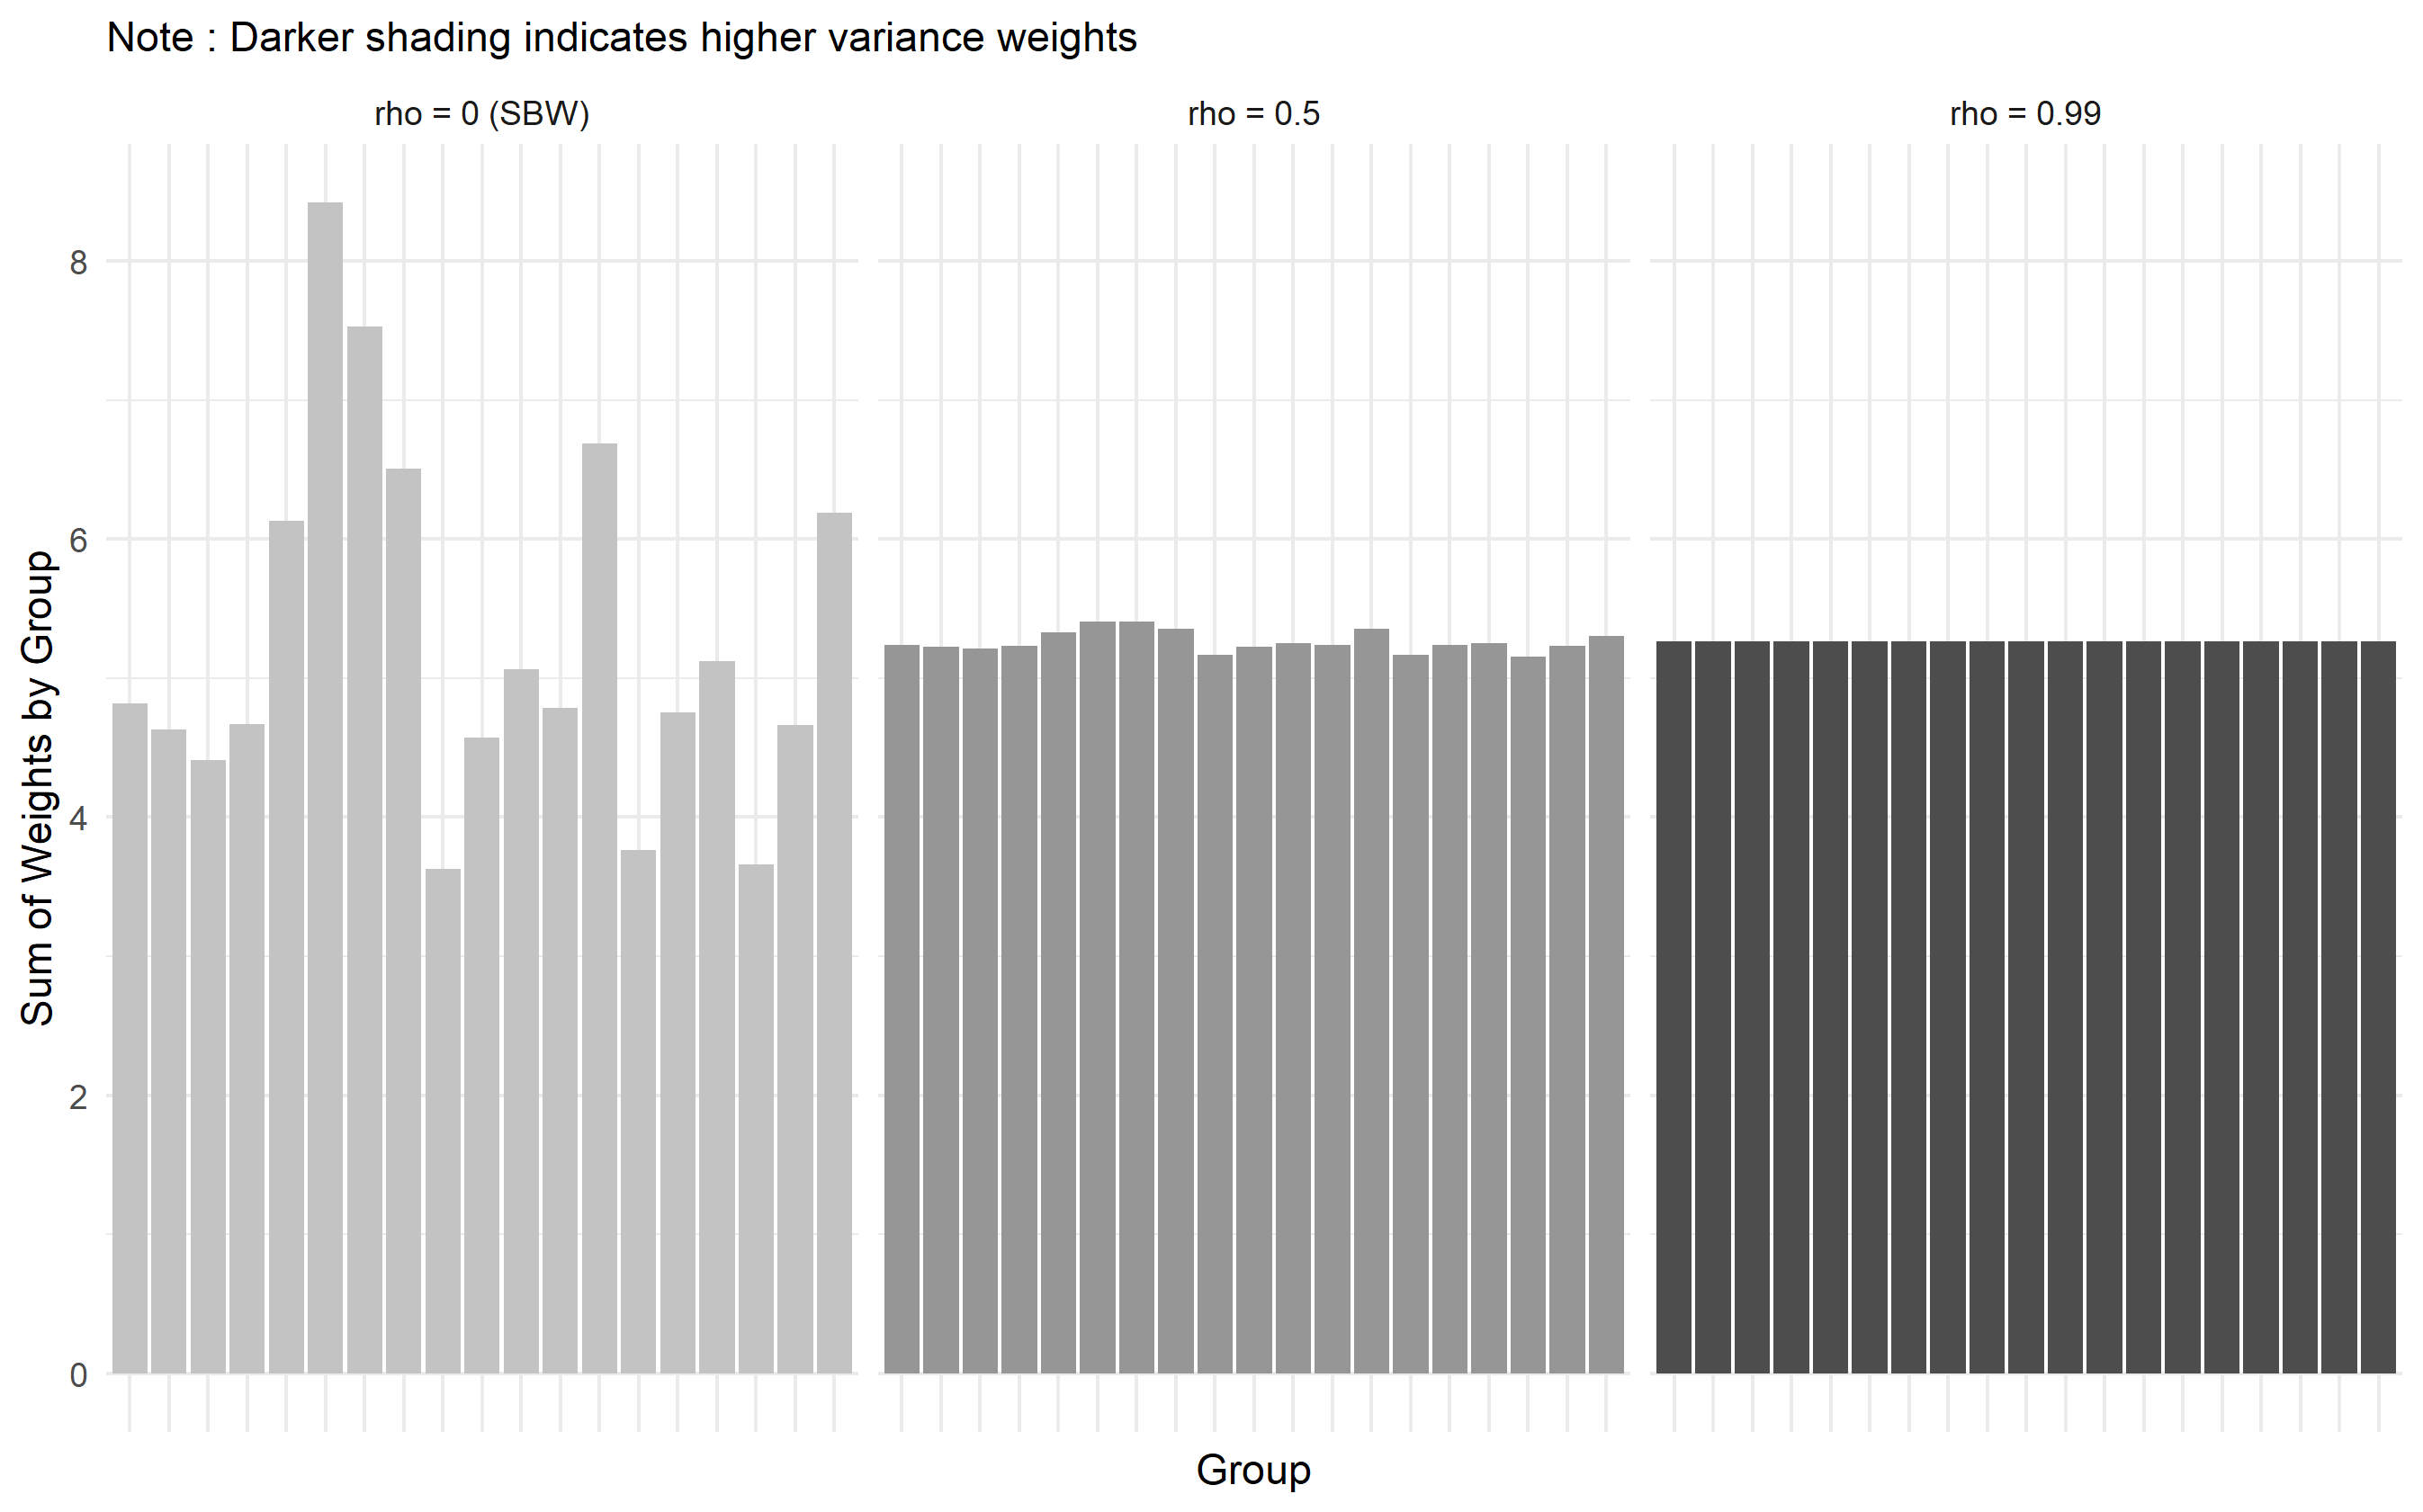
\includegraphics[scale=0.5]{01_Plots/proofofconcept.png}
    \caption{Comparison of SBW and H-SBW: within group sum of weights}
    \label{oatepref}
\end{center}
\end{figure}

In Appendix A we show that the H-SBW objective produces the minimum variance estimator under the constraint set for this correlation structure. In theory we could incorporate any assumed correlation structure into this objective in a similar fashion; however, the number of tuning parameters might change. Broadly speaking, we can think of H-SBW being to SBW what generalized least squares (GLS) is to ordinary least squares (OLS): both SBW and OLS can produce unbiased estimates of model parameters, but H-SBW and GLS can improve the efficiency of an estimator under different assumptions about the correlation structure of the outcomes.

\subsubsection{Measurement error}\label{ssec:methodsmsrment}

A second advancement in our estimation procedure comes in our balance constraints: rather than reweighting the observed covariates, we instead reweight the adjusted estimates $\hat{\eta}_1(W_{sc})$. This helps correct for the estimation error in the covariates that may bias the SBW estimate of $\bar{Y}_0^1$. In Appendix A, we consider the super-population target $\psi^1_0 = \mathbb{E}\{Y^1 \mid A = 0\}$ and show that under the classical errors-in-variables model, the bias for the SBW estimator that balances on the observed covariates $W$ and sets $\delta = 0$ is equivalent to the bias of a linear combination of coefficient estimates from the OLS-based regression estimator. Specifically, the bias for either estimator is:

\begin{equation}
\mathbb{E}\{\hat{\psi}^{1}_0 - \psi^1_0\} = (\upsilon_0 - \upsilon_1)^T(\kappa_1 - I_d)\beta_1
\end{equation}

The intuition for this result is as follows: exact balancing weights implicitly estimate $\beta_1$ on a subset of the data where we have sufficient covariate overlap. We can thus think of SBW as returning a solution to some weighted-least squares problem. Assuming that the outcome model holds across all of the data, WLS and OLS are estimating the same $\beta_1$; consequently, the bias that effects the least squares solution will have the same effect on the WLS, and therefore SBW, solution. In Appendix A, Proposition 2, we show that if we had access to $\eta_1$, we can obtain an unbiased estimate of $\psi^1$ by reweighting the adjusted covariates $\eta_1(W_{sc})$. Of course, in practice we do not know $\eta_1$ but must instead estimate it using auxillary data. In Appendix A, Proposition 3, we show that we can obtain a consistent of $\psi^1$ when balancing on an estimate of $\eta_1$ using auxillary data. 

The key is estimating $\eta_1$: at a high-level, we use the ACS micro-data replicate survey weights to estimate the covariance matrix of CPUMA sampling-variability $\Sigma_{vv, sc}$. Using our observed data to estimate $\Sigma_{WW \mid A = 1}$ and $\bar{X}_1$, we combine these estimates to generate an estimate of $\eta_1$. This is a technique that comes from the regression-calibration literature (see, e.g., \cite{gleser1992importance}). We also consider an adjustment procedure that further accounts for the differential measurement error due to the highly variable sample sizes used to calculate each covariate. This procedure allows our adjustment to differentially adjust covariate values depending on the sample-sizes involved in the adjustment procedure. We refer to the first procedure as ``homogeneous adjustment'' and the second procedure as ``heterogeneous adjustment'' since the adjustment is constant for all units in the first case, but varies by unit in the second case. Further details about these procedures are available in Appendix B. 

This is the first application we are aware of to apply regression calibration in the context of balancing weights to address the problem of measurement error. We emphasize two critical assumptions for using this procedure in our context: (1) the outcome model is linear in the true covariates; and (2) the measurement error in the outcome is uncorrelated with the measurement error in the covariates. The first assumption is strong, though often used in practice. The second assumption is reasonable in our setting, because the outcomes are estimated from a different cross-section than the covariates. 

\subsubsection{Bias-correction for imbalances}

In practice we are unable to reduce the balance constraints to our preferred level without generating very extreme weights. Following the recent literature on synthetic controls, we test the sensitivity of our results to the imbalances in the observed (or adjusted) covariates using ridge-regression augmented weights \cite{ben2018augmented}. Letting $\hat{X}_1$ be the matrix of adjusted covariates, and $\gamma^{hsbw}$ be our H-SBW weights, we consider the regression-augmented weights:

\begin{equation}
\gamma^{aug} = \gamma^{hsbw} + (\gamma^{hsbw}\hat{X}_1 - \bar{W}_0)^T(\hat{X}_1^T\Omega^{-1}\hat{X}_1 + \lambda I_q)^{-1}\hat{X}_1^T\Omega^{-1}
\end{equation}

where $\Omega$ is a block diagonal matrix with diagonal entries equal to one and the within-group off diagonals equal to $\rho$. We choose $\lambda$ so that all imbalances fall within 0.5 percentage points. The cost of this procedure is that we must extrapolate beyond the support of the data, making our estimates more model dependent. We refer to \cite{ben2018augmented} for more details about this procedure. For our results we consider estimators using SBW ($\rho = 0$), H-SBW ($\rho = 1/6$), and ridge-augmented versions of SBW and H-SBW that we call BC-SBW and BC-HSBW. 

\subsection{Model validation}

We previously argued that using pre-treatment outcomes to learn about variable importance may be misleading in this setting. The challenge again is that it is not obvious why the best model of $\bar{Y}_{0, t}^0$ for $t < T$ should also be the best model, or even a good model, of $\bar{Y}^1_{0,T}$. However, for fixed covariates and targeted levels of imbalance $\delta$, we use the heuristic that a good model of $\bar{Y}^1_{0,T}$ should also be a good model of $\bar{Y}_{0, t}^0$. We can also assume that when comparing two models, one with uniformly better covariate balance than the other, the model with uniformly better covariate balance should have lower bias both for $\bar{Y}_{0, T}^1$ and $\bar{Y}_{0, t}^0$ if our model assumptions are correct. We justify these comparisons by again assuming the outcome model is linear in $X$ for all time periods $t$. This is a stronger assumption than necessary to estimate the ETC, which only requires that $\mu_{1, T}$ is linear in $X$. However, these assumptions allow us to at least heuristically compare our models. 

Specifically, we rerun our procedures on pre-treatment data to compare the performance of our models for a fixed level of imbalances $\delta$. In particular, we train our model on 2009-2011 data to predict 2012 outcomes, and 2010-2012 data to predict 2013 outcomes. We limit to one-year prediction error since our estimand is only one-year forward. We then examine the performance of H-SBW against SBW, which vary with respect to the tuning parameter $\rho$, the bias-corrected versions, and the covariate adjustment procedure used in the balancing constraints. 

We expect that the estimators trained on the adjusted data should perform better than the estimators trained on the unadjusted data. If our outcome model is correct, these estimators should achieve better balance across the true covariates and therefore have lower bias than the estimators trained on the unadjusted data. We assume that any difference between the performance of the two adjustments is due to improved balance on the (unobserved) true covariates. For this comparison we do use the performance on this data to choose which adjustment we prefer for our final results. Conditional on the adjustment, we assume that if the bias-corrected estimators all have uniformly better covariate balance than the uncorrected estimators, these estimators should also perform better than the uncorrected estimators. However, if the assumed outcome models are incorrect, these estimators may suffer from extrapolation bias and perform worse despite achieving better balance. Finally, we expect SBW to have similar performance to H-SBW. We do expect to find the variance of H-SBW to be lower; however, we are only able to observe predictions on two years of pre-treatment data.

\subsection{Inference}

While placebo tests are frequently used in the synthetic controls literature for inference, we view these as qualitative statistical tests (see, e.g., \cite{arkhangelsky2019synthetic}) and instead use the leave-one-state-out jackknife to estimate the variance of $\hat{Y}_0^1$ (\cite{cameron2015practitioner}). Specifically, we exclude each state and re-calculate the weights holding our targeted mean fixed at $\bar{X}_0$ (using our estimate $\bar{W}_0$ and ignoring the variability associated with these estimates).\footnote{When our preferred initial choice of $\delta$ does not converge, we gradually reduce the constraints until it does.} We compute this estimate in two ways: first, we condition on our covariate adjustment $\hat{\eta}_1$. This is our preferred estimator; however, it does not account for the randomness in $\hat{\eta}_1$. We conduct a second procedure where we re-estimate $\hat{\eta}_1$ for each state omitted in the jackknife procedure and provide these results in Appendix E.

To estimate the variance of $\bar{Y}_0^0$ we use an auxillary regression model and use the CR-2 standard error adjustment to estimate the variance of the linear combination $\bar{W}_0^T\hat{\beta}_0$. We can estimate this quantity using the original (unadjusted) data given that $\mathbb{E}_W\{\bar{W}_0^T\hat{\beta}_0\} = \bar{Y}_0^0$ (since the regression line runs through the point $(\bar{W}_0, \bar{J}_0)$, which are unbiased estimates of $(\bar{X}_0, \bar{Y}_0)$). Our final estimate is the sum of these two variance estimates, and we use standard normal quantiles to generate confidence intervals. 

\section{Results}

We first present summary statistics regarding the variability of six time-varying covariates on our adjusted and unadjusted datasets. The second sub-section contains covariate balance diagnostics. The final sub-section contains our ETC estimates.

\subsection{Covariate adjustment}

Table~\ref{tab:adjust1} displays the effects of our covariate adjustment procedure on the variance of our pre-treatment outcomes and pre-treatment unemployment rates among the expansion states. We most heavily prioritize balancing these covariates, but they are also among the least precisely estimated (all of our other covariates average over multiple years of data). Table~\ref{tab:adjust1} displays the variance of each covariate on the unadjusted and adjusted datasets. We see that both the homogeneous and heterogeneous adjustment procedures reduce the variability in the data by comparable amounts. Intuitively, these adjustment reduce the likelihood that our balancing weights will over-fit to noise in the data. These results are consistent across most of our other covariates.

\begin{table}[ht]
\caption{Sample variance on unadjusted and adjusted datasets, expansion states}
\label{tab:adjust1}
\begin{tabular}{lrrr}
  \hline
Variable & No adjustment & Heterogeneous & Homogeneous \\ 
  \hline
Uninsured Pct 2011 & 8.35 & 8.04 & 8.05 \\ 
  Uninsured Pct 2012 & 8.20 & 7.89 & 7.90 \\ 
  Uninsured Pct 2013 & 8.09 & 7.78 & 7.79 \\ 
  Unemployed Pct 2011 & 3.66 & 3.25 & 3.27 \\ 
  Unemployed Pct 2012 & 3.72 & 3.38 & 3.38 \\ 
  Unemployed Pct 2013 & 3.20 & 2.88 & 2.87 \\ 
   \hline
\end{tabular}
\end{table}

\subsection{Covariate balance}

Figure~\ref{fig:loveplotc1} displays the reduction of imbalances using our H-SBW weights. This plot only displays covariates with greater than one percentage point difference between the targeted mean in the expansion region and the mean values in the non-expansion region prior to weighting, and the reweighted treatment values use our preferred covariate adjustment $\hat{\eta}_1(W_{sc})$. Before applying our weights, we see that there are substantial imbalances in the Republican governance indicators, as well as pre-treatment uninsurance and unemployment rates. Our weights reduce these differences; however, some remain, particularly among the Republican governance indicators. A complete balance table is available in Appendix D, Table 4. 

\begin{figure}[H]
\begin{center}
    \caption{Balance plot, primary dataset}
    \label{fig:loveplotc1}
    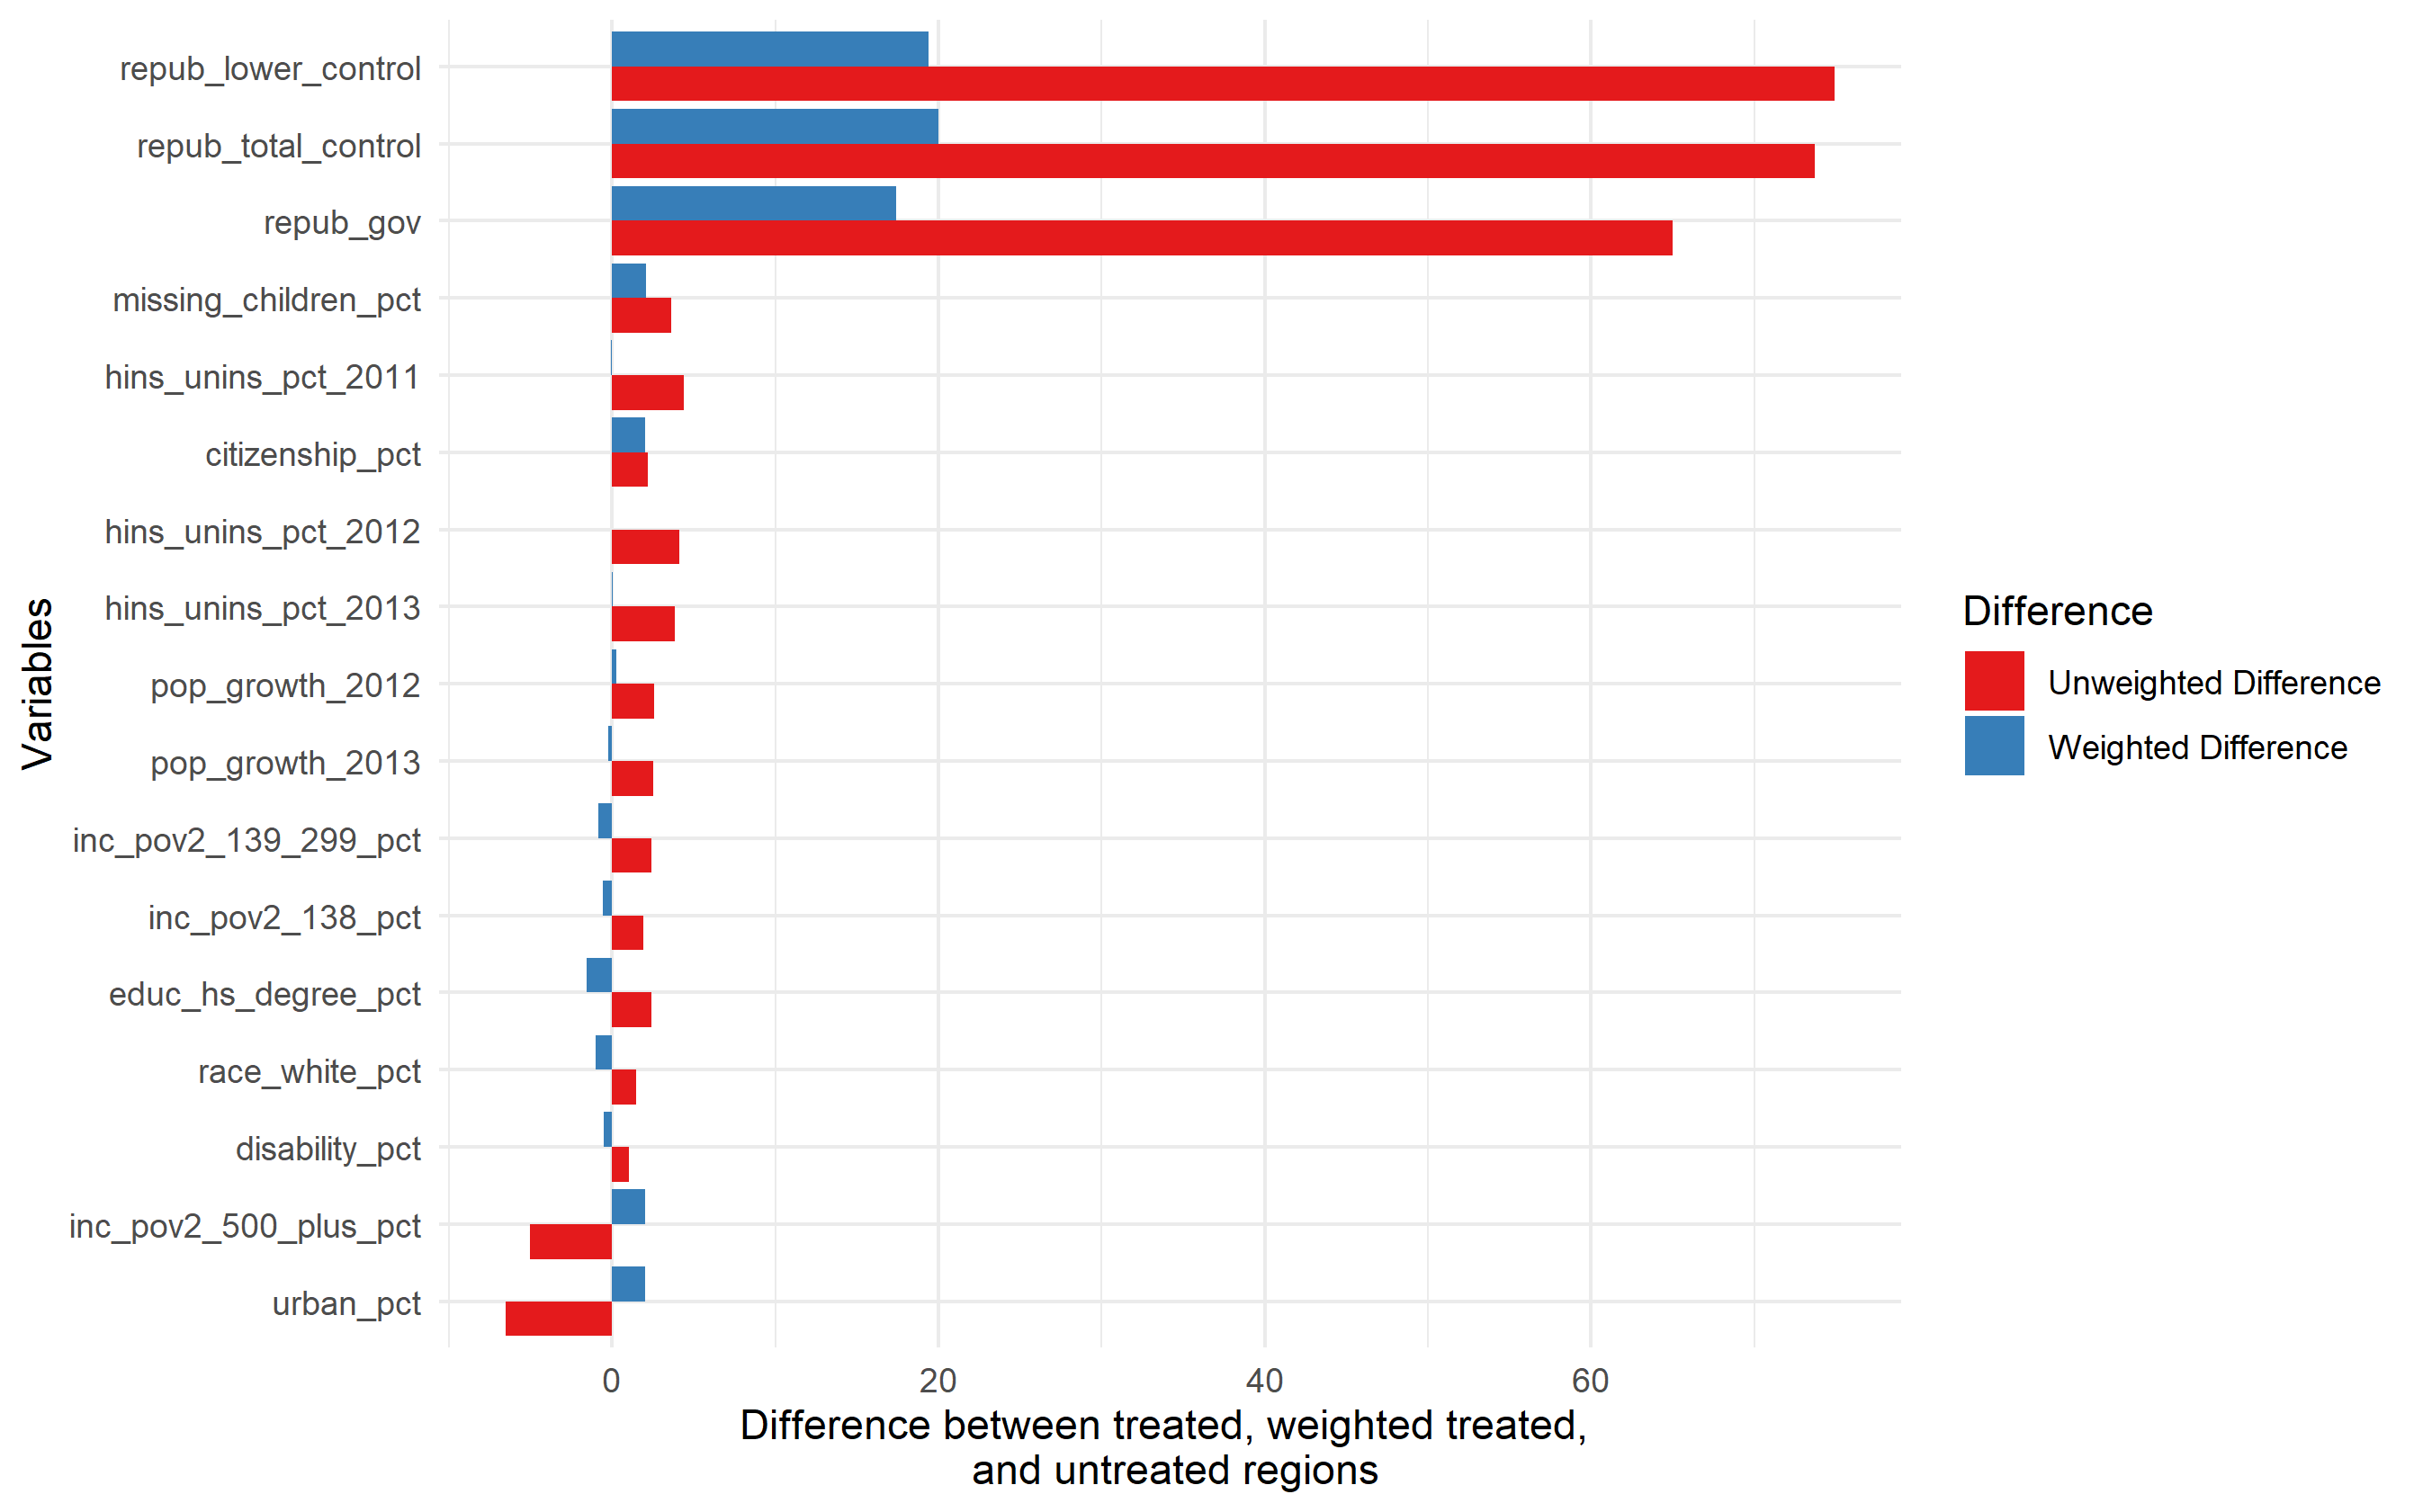
\includegraphics[scale=0.5]{01_Plots/balance-plot-etuc1.png}
\end{center}
\end{figure}

\begin{figure}[H]
\begin{center}
    \caption{H-SBW versus BC-HSBW versus SBW, weights summed by state, primary dataset}
    \label{fig:sbwvhsbw1}
    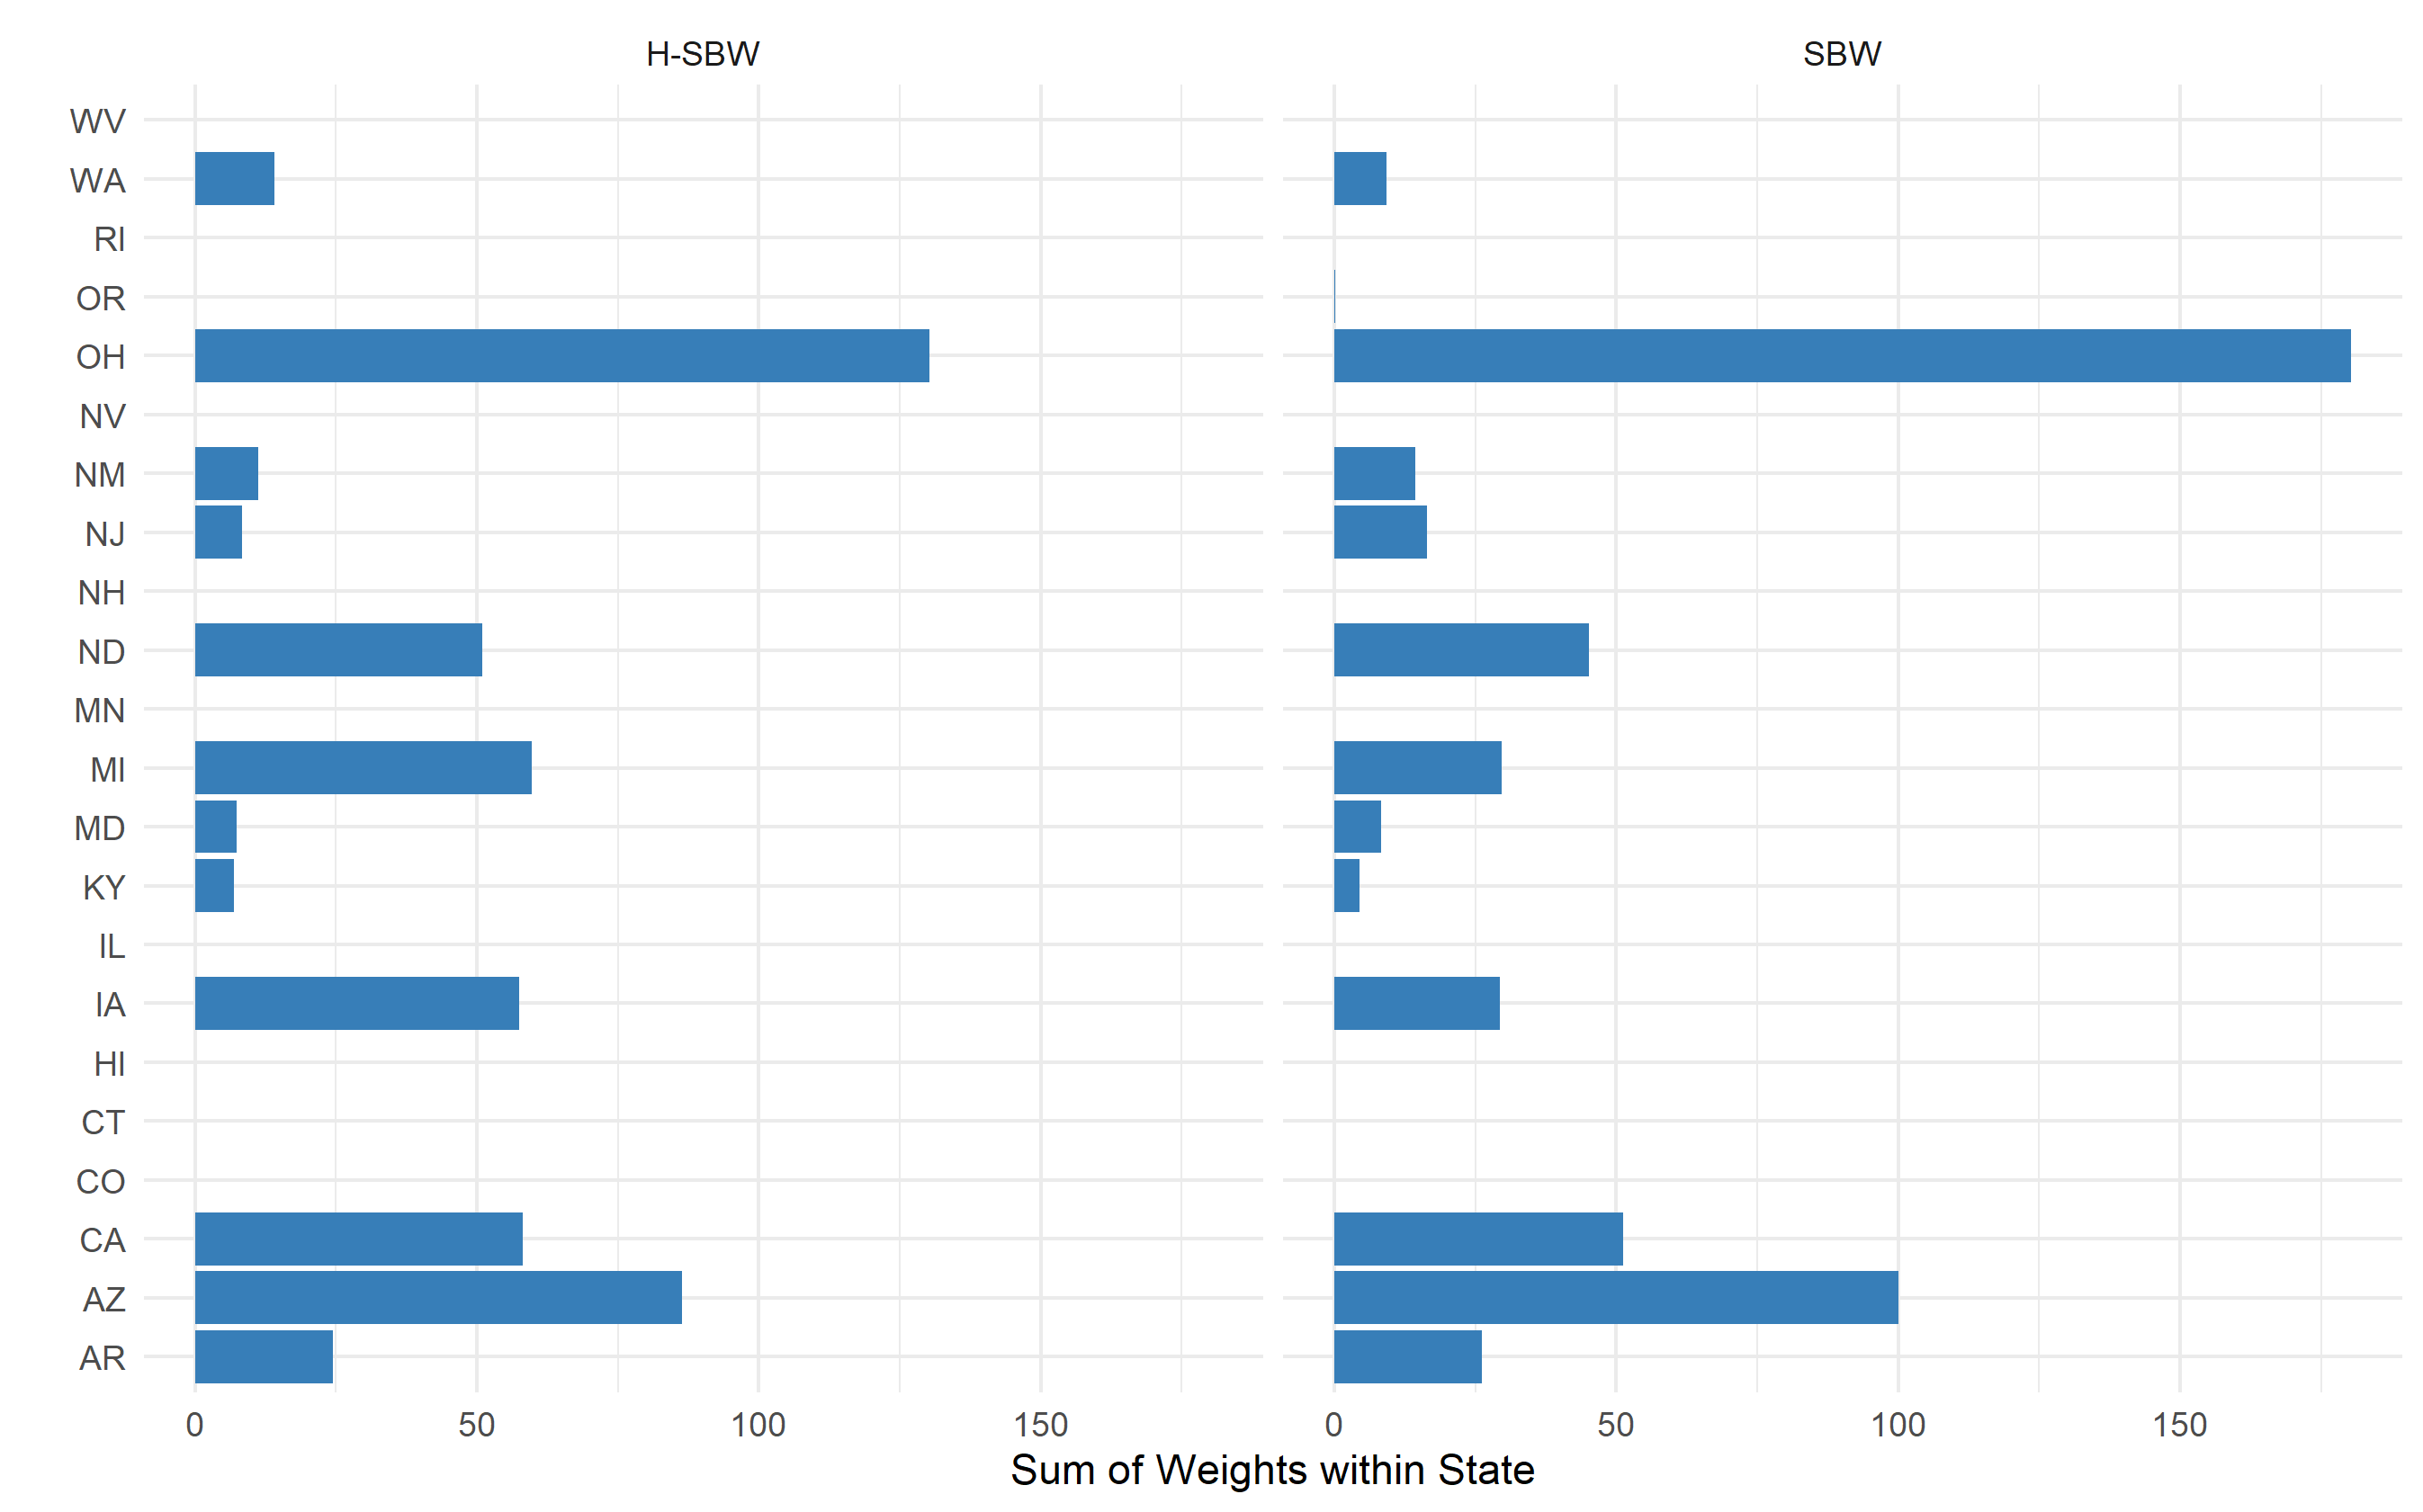
\includegraphics[scale=0.6]{01_Plots/weights-by-state-sbw-hsbw-c1.png}
\end{center}
\end{figure}

We then use ridge-regression augmentation to extrapolate from the data in order to reduce all imbalances within 0.5 percentage points. Figure~\ref{fig:sbwvhsbw1} shows the total weights summed across states for three estimators: H-SBW, BC-HSBW, and SBW. For BC-HSBW we display the negative weights separately from the positive weights to show the extent of the extrapolation. This figure illustrates two key points: first, that H-SBW more evenly disperses the weights across states relative to SBW; second, that BC-HSBW extrapolates somewhat heavily in order to achieve the desired level of balance, particularly for CPUMAs in California. 

Finally, we examine whether the H-SBW weights generated using the unadjusted data balance the adjusted covariates. While this metric does not reflect the ``true'' imbalances, the comparison gives some indication of whether the unadjusted weights are overfitting to noisy covariate measurements. [add sentence on what to expect] Table~\ref{tab:balcomp} compares the imbalances among our pre-treatment outcomes and uninsurance rates using H-SBW weights generated on our unadjusted dataset applied to the adjusted (homogeneous) dataset. The ``Unweighted Difference'' column represents the raw difference in means, while the ``Weighted Diff'' column reflects the weighted difference that we calculate on the unadjusted dataset. The ``Homogeneous Diff'' column displays the weighted imbalance when applying the H-SBW weights to the dataset using the homogeneous adjustment, and likewise for ``Heterogeneous Diff.'' The weighted pre-treatment outcomes are approximately one percentage point lower than we desired in the two years prior to treatment using the heterogeneous adjustment, and -0.2 percentage points lower (on average) using the homogeneous adjustment. Compared with the weighted difference (no adjustment) this is suggestive that the unadjusted weights are overfitting to noisy covariates and may give an overly optimistic view of balance obtained. Given the high degree of expected correlation between pre-treatment and post-treatment outcomes, we may expect the estimator of $\bar{Y}^1_0$ trained on the unadjusted data to have a downward bias.

\begin{table}[ht]
\caption{Balance comparison: weights estimated on unadjusted data applied to adjusted data}
\label{tab:balcomp}
\begin{tabular}{lrrrr}
  \hline
Variables & Unweighted Diff & Weighted Diff (none) & Homogeneous Diff & Heterogeneous Diff\\ 
  \hline
Uninsured Pct 2011 & -3.09 & -0.05 & -0.11 & 0.92 \\ 
  Uninsured Pct 2012 & -2.99 & -0.05 & -0.21 & -1.06 \\ 
  Uninsured Pct 2013 & -3.00 & -0.05 & -0.38 & -0.93 \\
   \hline
\end{tabular}
\end{table}

\subsubsection{Model validation}

We compare the performance of our models by repeating the covariate adjustments and calculating our procedure on 2009-2011 ACS data to predict 2012 outcomes, and similarly for 2010-2012 data to predict 2013 outcomes for the treated states. From Table~\ref{tab:pretxpred} we see that the estimators trained on the covariate adjusted data have substantially better performance than the unadjusted data. Moreover, the estimators trained on the homogeneous adjustment seem to do slightly better than the ones that model the heterogeneity; we present our results using the homogeneous adjustment. In thees earlier years we find that SBW tends to have slightly lower RMSE than H-SBW. However, the results are quite similar, as we expected. Finally, we see that the bias corrected estimators tend to perform worse in this application. This may indicate that the extrapolation bias outweighs the cost of reducing the covariate imbalances. While this does not imply that this model will perform badly when predicting $\bar{Y}^1_T$, it does suggest caution regarding these results. We see this as a function of our models being approximations: we expect in general that assuming the linear outcome models approximately holds on the support of the data where we have sufficient covariate overlap; however, these models may lead us astray when our weights extrapolate excessively from the data. The worst performing estimators are the bias-corrected estimators trained on the unadjusted data.

\begin{table}[ht]
\caption{Estimator pre-treatment outcome prediction error}
\label{tab:pretxpred}
\begin{tabular}{llrrr}
  \hline
Sigma estimate & Estimator & 2012 error & 2013 error & RMSE \\ 
  \hline
Homogeneous & SBW & -0.18 & -0.22 & 0.20 \\ 
  Homogeneous & H-SBW & -0.24 & -0.21 & 0.23 \\ 
  Heterogeneous & SBW & -0.25 & -0.30 & 0.27 \\ 
  Heterogeneous & H-SBW & -0.32 & -0.39 & 0.36 \\ 
  Homogeneous & BC-SBW & -0.42 & -0.35 & 0.39 \\ 
  Heterogeneous & BC-SBW & -0.45 & -0.39 & 0.42 \\ 
  None & SBW & -0.50 & -0.61 & 0.56 \\ 
  None & H-SBW & -0.52 & -0.61 & 0.57 \\ 
  Homogeneous & BC-HSBW & -0.53 & -0.62 & 0.58 \\ 
  Heterogeneous & BC-HSBW & -0.53 & -0.72 & 0.63 \\ 
  None & BC-SBW & -0.82 & -0.93 & 0.88 \\ 
  None & BC-HSBW & -0.93 & -0.99 & 0.96 \\ 
   \hline
\end{tabular}
\end{table}

We find a consistent negative bias across all of our estimators: all of our models tend to under-predict the true uninsurance rate among the non-expansion states the subsequent year by between a fifth to a whole percentage point. Assuming that the sign of this bias will also affect our estimates of $\bar{Y}^1_0$, we should expect our treatment effect estimates to have slight downward bias. That is, the true treatment effect may be smaller (closer to zero) in absolute magnitude than the estimated treatment effect. 

\subsection{Primary Results}

Using H-SBW we estimate an effect of -2.33 (-3.49, -1.16) percentage points. The SBW results are almost identical with -2.35 (-3.65, -1.06) percentage points. Compared to the unadjusted data we see very similar estimates at -2.34 (-2.85, -1.82) percentage points for H-SBW and -2.39 (-2.95, -1.83) percentage points for SBW. We see that H-SBW reduces the confidence intervals relative to SBW. We also observe that using the adjusted covariate set increases the width of the estimated confidence intervals. This increase in variability is expected because the adjustment procedure generally reduces the variability in the data, as we saw in Table~\ref{tab:adjust1}, thereby requiring that the balancing weights also increase in variability to achieve the desired level of balance. Importantly, this variance estimate conditions on the covariate adjustment, and does not take into account the randomness in this procedure, and may understate the true uncertainty. When we recalculate the entire adjustment procedure, we find that the confidence intervals are of a comparable magnitude. The results are available in Appendix E.

When we add the bias-correction, the absolute magnitude of the point estimate decreases: we estimate -2.05 (-3.32, -0.79) percentage points for BC-HSBW and -2.00 (-2.98, -1.01) percentage points for BC-SBW. Interestingly, in contrast to our validation tests, where the bias-corrected estimators tended to predict lower uninsurance rates than the other estimators, here the bias-correction predicts higher uninsurance rates for $\bar{Y}^1_0$. We also see that in contrast to the H-SBW and SBW estimators, the confidence interval for BC-SBW is narrower than for BC-HSBW. Table~\ref{tab:mainresults} presents all of our estimates, along with the results when excluding early expansion states. All adjusted estimates were closer to zero than the unadjusted estimates, though the point estimates from the SBW and H-SBW were estimators were virtually identical. We briefly note that the heterogeneous adjustments were all closer to zero than the unadjusted estimates. Complete results are available in Appendix E.

\begin{table}[ht]
\label{tab:mainresults}
\caption{Primary results}
\begin{tabular}{llll}
  \hline
Weight type & Adjustment & Estimate (95\% CI) & Early excluded estimate (95\% CI) \\ 
  \hline
H-SBW & Homogeneous & -2.33 (-3.49, -1.16) & -2.09 (-2.85, -1.33) \\ 
  H-SBW & None & -2.34 (-2.85, -1.82) & -2.28 (-2.82, -1.74) \\ 
  BC-HSBW & Homogeneous & -2.05 (-3.27, -0.82) & -1.94 (-2.96, -0.92) \\ 
  BC-HSBW & None & -2.22 (-2.87, -1.56) & -2.22 (-3.07, -1.38) \\ 
  SBW & Homogeneous & -2.35 (-3.65, -1.06) & -2.05 (-2.75, -1.35) \\ 
  SBW & None & -2.39 (-2.95, -1.83) & -2.21 (-2.71, -1.72) \\ 
  BC-SBW & Homogeneous & -2.07 (-3.17, -0.97) & -1.99 (-3.00, -0.99) \\ 
  BC-SBW & None & -2.19 (-2.90, -1.49) & -2.23 (-3.05, -1.40) \\ 
   \hline
\end{tabular}
\end{table}

We also consider the sensitivity of our analysis with respect to no anticipatory treatment effects. We exclude California, Connecticut, Minnesota, New Jersey, and Washington, which had partial expansions prior to 2014, and rerun our analyses. Figure 2 in Appendix D displays the H-SBW weights summed by state alongside BC-HSBW, which extrapolates to reduce the imbalances, and the results are available in Table~\ref{tab:mainresults}.

Our point estimates are similar to our primary analysis, though the numbers move slightly closer to zero. We also see that the differential between the estimates on the adjusted and unadjusted data is slightly larger: -2.28 (-2.82, -1.74) percentage points for H-SBW on the unadjusted dataset and -2.09 (-2.85, -1.33) on the adjusted data. We again find that when we add the bias-correction the point estimates again move closer to zero. Overall our primary results are relatively robust to the exclusion of these states. We conclude that potential violations of this causal assumption are not a large factor.

Lastly, we examine the robustness of our point estimates to the removal of individual states (these are the same point estimates used to calculate our confidence intervals). We find that removing Ohio tends to move the point estimates farther from zero, while removing North Dakota, Kentucky, or California tends to move the estimates closer to zero. Appendix E Figure 3 displays a heatmap showing how the estimates change for each estimator when removing each state.

\section{Discussion}

We estimate that had states that did not expand Medicaid in 2014 instead expanded their programs, they would have seen a -2.33 (-3.49, -1.16) percentage point change in the adult uninsurance rate. Existing estimates place the ETT between -3 and -6 percentage points. These estimates vary depending on the targeted sub-population of interest, the data used, the level of modeling (individuals or regions), and the modeling approach (see, e.g., \cite{courtemanche2017early}, \cite{kaestner2017effects}, \cite{frean2017premium}). Our estimate of the ETC are closer to zero than these ETT estimates. This difference may be a function of these different modeling strategies, or it may suggest that the ETC is smaller in absolute magnitude than the ETC. Regardless, due to the potential for effect heterogeneity, we emphasize the importance of directly estimating the targeted counterfactual of interest (e.g. the ETT or ETC), and being explicit about the assumptions used to estimate these quantities. We now consider our methodological contributions, study limitations, and we conclude by considering the policy implications of these findings.

\subsection{Methodological considerations}

We provide several methodological contributions to the literature on synthetic controls and balancing weights. First, we clarify some of the assumptions required to use synthetic controls to estimate the ETC. The challenge is that we need to predict treatment response rather than the outcome absent treatment. We emphasize that there may exist covariates that are weak confounders of the outcome absent treatment, but are strong confounders of the outcome under treatment.\footnote{In Appendix F we consider the role of Republican governance as an example, noting that \cite{kaestner2017effects} and \cite{courtemanche2017early} do not control for these factors when estimating their synthetic control weights. We show that these factors do substantially influence our estimates of $\bar{Y}_0^1$, though this does not rule out that these factors may also matter for predicting $\bar{Y}_1^0$.} While perhaps obvious, this point is not fully appreciated in the applied literature. For example, \cite{born2020lockdowns} recently used synthetic controls to estimate Sweden's COVID cases and deaths had they instituted a lockdown. The authors balance on pre-treatment infections, urbanization rate, and population size, and argue that the treatment is effectively random conditional on these covariates. While this may be true, the authors use the standard synthetic controls algorithm to generate their weights, using pre-treatment outcomes to determine the best model of the post-treatment counterfactual of $\bar{Y}^1_0$. For this application we forego this type of procedure and instead use our prior knowledge about the problem to prioritize covariate balance.

Second, our estimation procedure introduces and illustrates the H-SBW objective, which can improve upon the SBW objective when using hierarchical data. Assuming the errors in the outcome model follow the covariance structure posited by \cite{kloek1981ols}, H-SBW produces a lower variance estimator by more evenly dispersing weights across states. The assumption underlying the particular structure of our objective is that our model errors have constant variance and constant within-state correlation $\rho$. However, our procedure requires assuming the covariance structure and $\rho$ in advance. We choose $\rho = 1/6$ for this application. Identifying a data-driven approach to choose this tuning parameter (or perhaps for the covariance structure in general) could be a useful future contribution. 

Third, our estimation procedure accounts for measurement error in our covariates. We modify the constraint set to balance on a linear approximation to the true covariate values by adapting regression-calibration techniques (\cite{gleser1992importance}) to the balancing weights context. In Table~\ref{tab:balcomp} we show that the weights calculated on the unadjusted dataset fail to achieve the desired level of covariate balance on the adjusted dataset. We find that the weighted imbalances in our pre-treatment outcomes may be larger than we wanted, which we speculate for this application might bias our treatment effect downward. When we compared our estimates using the adjusted covariates to the unadjusted covariates, we find that our point estimates decrease (although often only slightly) in absolute magnitude. Essentially, when we generate weights on the unadjusted data to estimate the 2014 counterfactual outcome, they are likely fitting to noise, causing the observed level of balance to appear better than it truly is. Meanwhile, the re-weighted region may suffer from regression to the mean in the post-treatment period, making our treatment effect estimates appear larger in absolute magnitude than the truth. Once we adjust for the measurement error, our point estimates decrease in absolute magnitude (see also \cite{daw2018matching}, who discuss this phenomenon in more detail in the context of difference-in-differences designs). Overall, our study provides a roadmap for future studies that may wish to correct for potential measurement error while using balancing weights. 

One direction for further work is to calibrate this procedure to determine an optimal bias-variance tradeoff with respect to the measurement error. The procedure we implemented here was likely sub-optimal with respect to the mean-square error of our estimator. In particular, the bias induced by the measurement error decreases with square root of the sample size used to calculate each CPUMA's covariate values, the minimum of which were over three hundred. Meanwhile, the variance of our counterfactual estimate should decrease with the square root of the number of treated states (of which there are 21). From a theoretical perspective, the variance is of a larger order than the bias; moreover, adjusting for the bias will further increase the variance of the estimator. These concerns are consistent with our observed results: the change in our point estimates from the unadjusted data to the adjusted data is of a smaller magnitude than our variance estimate on our point estimate on the unadjusted data. Moreover, once we adjust for the measurement error, our confidence intervals increase more widely than the point estimates change.

\subsection{Limitations}

We caution that we required strong modeling assumptions throughout this analysis. In particular, we require SUTVA, no anticipatory treatment effects, no unmeasured confounding conditional on the true covariates, and several parametric assumptions about both the outcome and measurement error models. We were able to address some concerns about possible violations of these assumptions. For example, our results were qualitatively similar whether we excluded possible ``early expansion states,'' or used different weighting strategies (including relaxing the positivity restrictions and changing the tuning parameter $\rho$). We also examined two versions of our covariate adjustment and found similar results with either. However, we do not attempt to address concerns about SUTVA violations, particularly the impact of spillovers across regions. And while we believe that no unmeasured confounding is reasonable for this problem, we did not conduct a sensitivity analysis (see, e.g., \cite{bonvini2021sensitivity}) with respect to this assumption.

\subsection{Policy considerations}

We find that our point estimates for the ETC are somewhat smaller in absolute magnitude than existing estimates of the ETT. While we make no formal statistical claims about these differences, this finding nevertheless highlights the importance of caution when using estimates of the ETT to make inferences about the ETC. Because almost every outcome of interest is mediated through increasing the number of insured individuals, if the ETC is in fact different than the ETT, then projecting findings from an estimate of the ETT to the ETC may lead to inaccurate inference. For example, \cite{miller2019medicaid} study the effect of Medicaid expansion on mortality. Using their estimate of the ETT they project that had all states expanded Medicaid, 15,600 deaths would have been avoided during their study's time-period. If we believe that this number increases monotonically with the number of uninsured individuals, this estimate may be an overestimate if the ETC is less than the ETT, or an underestimate if the ETC is greater than the ETT. Directly estimating the ETC can help us better model policy relevant downstream effects mediated through decreasing the uninsurance rate. 

Medicaid expansion is also still an ongoing policy debate in the United States. Following the passage of the American Rescue Plan, state legislatures in Wyoming, Alabama, and North Carolina are reportedly considering expanding their programs. Our study estimates the effect of Medicaid expansion on adult uninsurance rates; however, this effect is only interesting because Medicaid enrollment is not automatic for eligible individuals. Different state policies may therefore make it easier or harder to enroll in Medicaid. We emphasize that if the goal of Medicaid expansion is to increase insurance access for low-income adults, state policy-makers also may wish to make it easier to enroll in Medicaid. 

\section{Conclusion}

This is the first study we are aware of that directly estimates the foregone coverage expansions of Medicaid expansion on states that did not expand Medicaid in 2014. Our estimation approach contributes to the methodological literature on synthetic controls by outlining a set of identifying assumptions to estimate the ETC rather than the ETT, and to the balancing weights literature by using an estimation procedure that account for hierarchical data structure and measurement error in the covariates. We estimate that had states that did not expand their Medicaid eligibility requirements in 2014 done so, they would have seen a -2.33 (-3.49, -1.16) percentage point change in their uninsurance rate. This point estimate is closer to zero than existing estimates of the ETT, which range between -3 and -6 percentage points (\cite{frean2017premium}).\footnote{As we noted above, prior studies differ with respect to the data used, the targeted population of interest, the modeling choices, and unit level of analysis.} From a policy-analysis perspective, we caution against using using existing estimates of the ETT to make inferences about the ETC. From a policy-making standpoint, we note that if the goal of Medicaid expansion is to increase access to insurance for low-income adults, state and federal policy-makers may wish to consider policies that make Medicaid enrollment easier if not automatic.

\section*{Acknowledgements}

The authors gratefully acknowledge invaluable advice and comments from Zachary Branson, Dave Choi, Edward Kennedy, Brian Kovak, Akshaya Jha, Lowell Taylor, and Jose Zubizaretta.

\begin{supplement}
Analysis programs and supporting materials are available online at github.com /mrubinst757/medicaid-expansion. Proofs and additional results are available in the Appendix.
\end{supplement}

\bibliographystyle{imsart-nameyear} % Style BST file
\bibliography{research.bib}       % Bibliography file (usually '*.bib')

\clearpage

\appendix
\section{Proofs}\label{ssec:proof}

We divide our proofs into three sections: the first two consist of propositions and the third contains the proofs of the propositions. In the first section our propositions pertain to the performance of SBW under the classical measurement error model. Our key results are that the bias of the SBW estimator is equivalent to the bias of the OLS estimator and that regression-calibration techniques can be used in this setting to obtain consistent estimators. However, these results assume that the data are gaussian. We also show that if the data are not gaussian, the OLS estimator using regression-calibration remains consistent, while the SBW estimator may be biased. In our second section we consider the properties of the H-SBW objective when the true covariates $X$ are observed. We show that if our assumed correlation structure for the outcome errors is correct, H-SBW produces the minimum conditional-on-X variance estimator within the constraint set. We also show how a generalized form of H-SBW weights relate to the implied regression weights from Generalized Least Squares (GLS). We conclude by showing that H-SBW may yield biased estimates if we do not correctly model the dependence structure of the data. Section~\ref{app:AsecIII} contains all of the proofs.

\subsection{SBW and classical measurement error}\label{app:AsecI}

We begin by showing six results regarding the bias of the OLS and SBW estimators under the classical errors-in-variables model. First, we show that without adjustment for errors-in-covariates, the bias of the SBW estimator that sets $\delta = 0$ (i.e. reweights the treated units to exactly balance the control units) is equal to the bias of the OLS estimator. Second, we show that if the observed covariate values for the treated data can be replaced by their conditional expectations $\tilde{X}$ given the noisy observations, then the SBW estimator will be unbiased and consistent. Third, we consider the case where $\tilde{X}$ must be estimated, and show that the SBW estimator is consistent if we replace $\tilde{X}$ by a consistent estimate $\hat{X}$. Finally, we remove the assumption that $X$ is gaussian, and show that while the OLS estimator remains unbiased under weaker assumptions, the SBW estimator does not, and we show a general expression for the asymptotic bias. We take the perspective throughout that $X$ is random among the treated units but fixed for the control units.

We assume that equations (\ref{eqn:unconfoundedness}) - (\ref{eqn:Xgaussian}) hold. For simplicity, we additionally assume that
\begin{equation}\label{eqn:simplifications}
\epsilon_{sc} = 0, \quad \varepsilon_s = 0,\quad \xi_{sc} = 0,\quad  \Sigma_{\nu,sc} = \Sigma_\nu, \qquad \forall s,c
\end{equation}
noting that $\xi_{sc}=0$ implies $J_{sc} = Y_{sc}$. The covariate observations of the treated units can then be seen to be i.i.d., with covariance matrix
\[ \Sigma_{W|1} = \Sigma_{X|1} + \Sigma_\nu,\]
and the conditional expectation of $X_{sc}$ given $W_{sc}$ for the treated units can be seen to equal
\[ \tilde{X}_{sc} = v_1 + \kappa^T (W_{sc} - v_1), \qquad \forall sc: A_{sc}=1,\]
where
\[ \kappa = (\Sigma_{X|1} + \Sigma_{\nu})^{-1} \Sigma_{X|1}.\]
To ease notation, we abbreviate $\Sigma_X = \Sigma_{X \mid 1}$ and similarly $ \Sigma_W = \Sigma_{W \mid 1}$. 

In Propositions \ref{cl8}, \ref{cl9}, and part of Proposition \ref{cl1}, we will remove the Gaussian covariate assumption given by \eqref{eqn:Xgaussian}. In its place, we will instead consider the weaker assumption that the empirical covariance of $X$ has a limit $S_X$,

\begin{equation}\label{eqn:limitX}
 \frac{1}{n_1} \sum_{A_{sc}=1} (X_{sc} - \bar{X}_1)(X_{sc} - \bar{X}_1)^T \rightarrow^p S_X,
\end{equation}
which implies a similar limit $S_W$ for the noisy observations $W$,

\begin{equation}\label{eqn:limitW}
 \frac{1}{n_1} \sum_{A_{sc}=1} (W_{sc} - \bar{W}_1)(W_{sc} - \bar{W}_1)^T \rightarrow^p S_W = S_X + \Sigma_{\nu},
\end{equation}
where we have used the independence of the noise terms $\nu_{sc}$, and similarly that 
\begin{equation}\label{eqn:limitWY}
 \frac{1}{n_1} \sum_{A_{sc}=1} (W_{sc} - \bar{W}_1)(Y_{sc} - \bar{Y}_1)^T \rightarrow^p S_X \beta_1,
\end{equation}
where we have additionally used the linear model for $Y_{sc}$ given by \eqref{eqn:linmod}.

We first consider estimation without adjustment for errors in covariates. 
Proposition \ref{cl1} states that the unadjusted OLS and SBW estimators have equal bias, with the bias of the OLS estimator remaining unchanged if the gaussian assumption of \eqref{eqn:gaussiannoise} is removed.

\begin{proposition}\label{cl1}
Let (\ref{eqn:unconfoundedness}) - (\ref{eqn:Xgaussian}) and (\ref{eqn:simplifications}) hold.
Let $(\hat{\alpha}, \hat{\beta})$ denote the unadjusted OLS estimator of $(\alpha_1, \beta_1)$, 
\begin{equation}\label{eqn:prop1.beta}
(\hat{\alpha}, \hat{\beta}) = \arg \min_{\alpha, \beta} \sum_{sc:A_{sc}=1} (Y_{sc} - \alpha -  W_{sc}^T\beta)^2,
\end{equation}
which induces the OLS estimator of $\psi_0^1$ given by

\begin{align*}
\hat{\psi}^{1,\textup{ols}}_0 = \bar{Y}_1 + (\bar{W}_0 - \bar{W}_1)^T\hat{\beta}_1.
\end{align*}
%
Let ${\gamma}$ denote the unadjusted SBW weights under exact balance, found by solving \eqref{eqn:SBWobjective} with constraint set $\Gamma( W_{A=1}, \bar{W}_0, 0)$, which induces the SBW estimator of $\psi_0^1$ given by

\begin{align*}
\hat{\psi}^{1,\textup{sbw}}_0 = \sum_{sc: A_{sc} = 1} {\gamma}_{sc} Y_{sc}.
\end{align*}
%
Then the estimators $\hat{\psi}^{1, \textup{ols}}_0$ and $\hat{\psi}^{1, \textup{sbw}}_0$ have equal bias, satisfying

\begin{align*}
\mathbb{E}[\hat{\psi}_0^{1,\textup{ols}}] &= \mathbb{E}[\hat{\psi}^{1, \textup{sbw}}_0]  = \psi_0^1 + (\bar{X}_0 - \upsilon_1)^T(\mathbf{\kappa} - I_q)\beta.
\end{align*}
Additionally, the bias of $\hat{\psi}_0^{1,\textup{ols}}$ is asymptotically unchanged if the gaussian covariate assumption given by \eqref{eqn:Xgaussian} is replaced by \eqref{eqn:limitX}.
\end{proposition}

To study the SBW estimator with covariate adjustment, we first consider an idealized version where $\Sigma_X$ and $\Sigma_\nu$ are known, so that $\tilde{X}_{A=1}$ is also known. Proposition \ref{cl2} shows that the resulting estimate of $\psi_0^1$ is unbiased if $\delta = 0$.

\begin{proposition}\label{cl2}
Let (\ref{eqn:unconfoundedness}) - (\ref{eqn:Xgaussian}) and (\ref{eqn:simplifications}) hold. Let $\tilde{X}_{A=1}$ equal the conditional expectation of $X_{A=1}$ given $W$,

\[ \tilde{X}_{sc} = \upsilon_1 + \kappa^T (W_{sc} - \upsilon_1), \qquad \forall sc: A_{sc} = 1,\] let $\gamma^*$ be the solution to the SBW objective defined over the constraint set $\Gamma(\tilde{X}_{A=1}, \bar{X}_0, 0)$, and let $\hat{\psi}^{1, \textup{ideal}}_0$ be the SBW estimator $\sum_{sc: A_{sc} = 1}\gamma^\star_{sc}Y_{sc}$. This estimator is unbiased for $\psi_0^1$.
\end{proposition}



Proposition \ref{prop:variance_rate} shows that the variance of this idealized SBW estimator goes to zero, implying consistency. 
\begin{proposition}\label{prop:variance_rate}
Let (\ref{eqn:unconfoundedness}) - (\ref{eqn:Xgaussian}) and (\ref{eqn:simplifications}) hold, and let $\gamma^*$ and $\hat{\psi}_0^{1, \textup{ideal}}$ be defined as in Proposition \ref{cl2}. Then the conditional variance of the estimation error is given by

\begin{align*}
\operatorname{Var}\left( \hat{\psi}_0^{1, \textup{ideal}} - \psi_0^1| W\right)  = \|\gamma^*\|^2 \cdot \beta_1^T(\Sigma_{X} - \Sigma_{X}\Sigma_{W}^{-1}\Sigma_{X})\beta_1, 
\end{align*}
with $\operatorname{Var}\left( \hat{\psi}_0^{1, \textup{ideal}} - \psi_0^1| W\right)$ and $\operatorname{Var}(\hat{\psi}_0^{1,\textup{ideal}})$ both behaving as $O_P(n_1^{-1})$ as $n_1 \rightarrow \infty$.
\end{proposition}

In practice, the idealized SBW estimator considered in Propositions \ref{cl2} and \ref{prop:variance_rate} cannot be used, as $\Sigma_X$ and $\Sigma_{\nu}$ are not known, but instead must be estimated from auxilliary data. Proposition \ref{cl3} states that if these estimates are consistent, then the resulting adjusted SBW estimator for $\psi_0^1$ is also consistent if $\delta = 0$.

\begin{proposition}\label{cl3}
Let (\ref{eqn:unconfoundedness}) - (\ref{eqn:Xgaussian}) and (\ref{eqn:simplifications}) hold. Given estimates $\hat{\Sigma}_X$ and $\hat{\Sigma}_\nu$ that are consistent for $\Sigma_X$ and $\Sigma_\nu$, let $\hat{X}_{A=1}$ be given by 
\[ \hat{X}_{sc} = \bar{W}_1 + \hat{\kappa}^T(W_{sc} - \bar{W}_1), \]
where $\hat{\kappa} = (\hat{\Sigma}_X + \hat{\Sigma}_{\nu})^{-1} \hat{\Sigma}_X$. Let $\hat{\gamma}$ be the weights that solve the SBW objective over the constraint set $\Gamma(\hat{X}_{A=1}, \bar{W}_0, 0)$, and let $\hat{\psi}^{1, \textup{adjusted}}_0 = \sum_{sc: A_{sc} = 1} \hat{\gamma}_{sc} Y_{sc}$ be the corresponding SBW estimator. This estimator is consistent for $\psi_0^1$ as $n_1 \to \infty$.
\end{proposition}

In (\ref{eqn:jackknife}) we propose a leave-one-state-out jackknife estimate of variance. Following \cite{efron1981jackknife}, this estimate can be decomposed a conservatively biased estimate of the variance of $\hat{\psi}_0^{1, \textup{adjusted}}$ given a sample size of $(m_1-1)$ treated states, plus a heuristic adjustment to go from sample size $(m_1-1)$ to sample size $m_1$, when treating the observations of the control states as fixed.

\begin{proposition}\label{prop:jackknife}
Let (\ref{eqn:unconfoundedness}) - (\ref{eqn:gaussiannoise}) hold, and additionally assume that $p_s$, the number of CPUMAs, is i.i.d. in the treated states. Let $\hat{\operatorname{Var}}(\hat{\psi}_0^{1, \textup{adjusted}}) = \frac{m_1-1}{m_1} \cdot \tilde{\operatorname{Var}}(\hat{\psi}_0^{1, \textup{adjusted}})$, where

\begin{equation} \label{eqn:prop.jackknife}
\tilde{\operatorname{Var}}(\hat{\psi}_0^{1, \textup{adjusted}}) = \sum_{s:A_{s}=1} (S_{(s)} - S_{(\cdot)})^2,
\end{equation}
with $S_{(s)}$ and $S_{(\cdot)}$ as defined for \eqref{eqn:jackknife}. Then $\tilde{\operatorname{Var}}$ is conservatively biased for the variance of the leave-one-state-out estimate,

\[ \mathbb{E}\left[ \tilde{\operatorname{Var}}(\hat{\psi}_0^{1, \textup{adjusted}})\right] \geq \operatorname{Var}(S_{(1)} | \bar{W}_0),\]
where $S_{(1)}$ can be seen to equal the estimator $\hat{\psi}_0^{1,\textup{adjusted}}$ under a sample size of $(m_1-1)$ treated states.

\end{proposition}

As the gaussian covariate assumption given by \eqref{eqn:Xgaussian} is strong, it would be desirable if the adjusted OLS or SBW estimators were consistent even for non-gaussian $X$. Proposition \ref{cl8} shows under mild assumptions that this is in fact true when running OLS on the adjusted covariates. 

\begin{proposition}\label{cl8}
Let (\ref{eqn:unconfoundedness}) - (\ref{eqn:gaussiannoise}), and (\ref{eqn:simplifications})- (\ref{eqn:limitX}) hold, with $S_X$ invertible. Let $(\check{\alpha}, \check{\beta})$ denote the adjusted OLS estimates of $(\alpha_1, \beta_1)$, solving

\[ \min_{\alpha,\beta} \sum_{A_{sc}=1} (Y_{sc} - \alpha - \check{X}_{sc}^T \beta)^2, \]
where $\check{X}_{sc} = \bar{W}_1 + \check{\kappa}^T(W_{sc} - \bar{W}_1)$ with $\check{\kappa} = (S_X + \Sigma_\nu)^{-1}S_X$. Then the adjusted OLS estimator of $\psi_0^1$ given by
\[ \bar{Y}_1 - (\bar{W}_0 - \bar{W}_1)^T \check{\beta},\]
remains consistent if the gaussian assumption given by \eqref{eqn:gaussiannoise} is removed.
\end{proposition}

However, the same does not hold for the adjusted SBW estimator. Proposition \ref{cl9} gives an expression for its bias when the covariates are non-gaussian. 

\begin{proposition}\label{cl9}
Let the assumptions of Proposition \ref{cl8} hold. Let $\check{\gamma}$ solve the SBW objective over the constraint set $\Gamma(\check{X}_{A=1}, \bar{W}_0, 0)$ where $\check{X}_{A=1}$ and $\check{\kappa}$ are defined as in Proposition \ref{cl8}. Let $Q$ denote the set of indices where $\check{\gamma}$ is non-zero,

\[ Q = \{sc: \check{\gamma}_{sc} > 0\},\]
with cardinality $n_Q = |Q|$, and let $\bar{W}_Q$ and $S_{W_Q}$ denote the empirical mean and covariance of $\{W_{sc}:sc \in Q\}$,

\[ \bar{W}_Q = \frac{1}{n_Q}\sum_{sc \in Q} W_{sc},\qquad S_{W_Q} = \frac{1}{n_Q} \sum_{sc \in Q} (W_{sc} - \bar{W}_Q)(W_{sc} - \bar{W}_Q)^T,\]
with $\bar{X}_Q$ the analogous empirical mean of $\{X_{sc}:sc \in Q\}$ and $S_{XW_Q}$ the empirical cross covariance,
\[ S_{XW_Q} = \frac{1}{n_Q} \sum_{sc \in Q} (X_{sc} - \bar{X}_Q)(W_{sc} - \bar{W}_Q)^T.\]
Then if the gaussian assumption given by \eqref{eqn:gaussiannoise} is removed, the adjusted SBW estimator for $\psi_0^1$ given by 

\[\sum_{A_{sc}=1} Y_{sc} \check{\gamma}_{sc},\]
may be biased for $\psi_0^1$, with estimation error given by 

\begin{align} 
\nonumber \sum_{A_{sc}=1} Y_{sc} \check{\gamma}_{sc} - \psi_0^1 & = \beta_1^T\Big[(S_{XW_Q}S_{W_Q}^{-1}S_WS_X^{-1} - I)\bar{X}_0  + (\bar{X}_Q - S_{XW_Q}S_{W_Q}^{-1} S_W S_X^{-1} \bar{X}_1) \\
& \hskip1cm {} - S_{XW_Q}S_{W_Q}^{-1}(\bar{X}_Q - \bar{X}_1)\Big](1 + o_P(1)),  \label{eqn:cl9.error}
\end{align}
which need not converge to zero unless $\bar{X}_Q \to \bar{X}_1$, $S_{XW_Q} \to S_X$, and $S_{W_Q} \to S_W$.
\end{proposition}

Proposition \ref{cl7} shows that if the conditional expectations can be computed for the treated units (which may be computationally difficult or require strong modeling assumptions if the data is non-gaussian, or if dependencies exist between CPUMAs), then SBW yields unbiased estimates. 

\begin{proposition}\label{cl7}
    Let equations (\ref{eqn:unconfoundedness})-(\ref{eqn:linmod}) hold. Let $\tilde{X}^*$ denote the conditional expectation,
    \[\tilde{X}^*_{sc} = \mathbb{E}[X_{sc} | W, A_{sc}=1],\]
    let weights $\tilde{\gamma}^*$ solve the SBW objective (\ref{eqn:SBWobjective}) with constraint set $\Gamma(\tilde{X}^\star_{A=1}, \bar{X}_0, 0)$, and consider the estimator of $\psi_0^1$ given by $\sum_{A_{sc}=1} Y_{sc} \tilde{\gamma}^*_{sc}$. This estimator is unbiased for $\psi_0^1$.
\end{proposition}

\begin{remark}
    While we have assumed that $\epsilon_{sc}=0$ for simplicity in our propositions, removing this assumption simply leads to the additional term $\sum_{sc: A_{sc} = 1}\gamma_{sc}\epsilon_{sc}$ in the error of the SBW estimator of $\psi_0^1$. This again has expectation zero, because the weights remain independent of the error $\epsilon_{sc}$ in the outcomes. Allowing non-zero $\epsilon_{sc}$ also adds a term to the estimator variance (conditional on $W$) equal to $\sigma^2_{\epsilon}\cdot \|\gamma^*\|^2$,    which does not change the variance bound given by Proposition \ref{prop:variance_rate}.
\end{remark}


\begin{remark}
    For the adjusted OLS estimator, in which $\beta_1$ is estimated using the adjusted covariates $\tilde{X}_{A=1}$, in practice we must estimate $\tilde{X}$ with some estimator $\hat{X}$ that relies on an estimate $\hat{\kappa}$. As long as $\hat{\kappa}$ is consistent for $\kappa$ then the OLS estimator will also be consistent by the continuous mapping theorem.
\end{remark}

\begin{remark}
As the proposition implies that $\hat{\operatorname{Var}}$ is conservatively biased only up the heuristic $(m_1-1)/m_1$ scaling term, it may be preferable to remove this term, inflating the variance estimate slightly. While Proposition \ref{prop:jackknife} considers the marginal variance of the estimator $\hat{\psi}_0^{1,\textup{adjusted}}$, a confidence interval using the conditional variance $\operatorname{Var}(\hat{\psi}_0^{1 \textup{adjusted}}|X)$ (see, e.g., \cite{buonaccorsi2010measurement}, who discuss using a modification of the parametric bootstrap for parameters estimated via OLS in this setting) may be of interest, potentially leading to smaller intervals and more precise inference. 
\end{remark}


\begin{remark}
To see how Proposition \ref{cl9} implies that the adjusted SBW estimate may be biased in non-gaussian settings, we observe that as the set $Q$ in Proposition \ref{cl9} will depend on the values of the covariates $X$ and observation noise $\nu$, the values of $\{X_{sc}: sc \in Q\}$ and $\{\nu_{sc}: sc \in Q\}$ may differ systematically from their population, so that $\bar{X}_Q$, $S_{XW_Q}$ and $S_{W_Q}$ may not converge to their desired counterparts. While the expression for the estimation error given by (\ref{eqn:cl9.error}) is asymptotic, an exact formula is given in  \eqref{eqn:cl9.proof3} which is very similar; the only asymptotic approximations are the convergence of $\bar{W}_1$ to $\bar{X}_1$ and $\bar{W}_0$ to $\bar{X}_0$. Proposition \ref{cl7}, presented in the next section, suggests an approach to restore unbiased estimation for SBW and H-SBW in non-gaussian settings.
\end{remark}

\begin{remark}\label{remark:basis expansion}
We describe a possible direction for future work that utilizes Proposition \ref{cl7}. Suppose that in lieu of equations  (\ref{eqn:additivenoise})-(\ref{eqn:Xgaussian}), we instead assume that $X_{sc}$ is a transformation of the covariate, so that $X_{sc} = \phi(U_{sc})$ for some transformation $\phi$, and that the untransformed $U_{sc}$ is observed with additive noise, so that $W_{sc} = U_{sc} + \nu_{sc}$. For example, to make the linear model (\ref{eqn:linmod}) more credible, $\phi(U_{sc})$ might denote a basis expansion applied to the survey sampled covariates for each unit. If, analogous to assumptions (\ref{eqn:gaussiannoise}) and (\ref{eqn:Xgaussian}), the original covariates $U_{sc}$ and measurement error $\nu_{sc}$ can be assumed to be iid gaussian, so that the treated units satisfy

\begin{align*}
    U_{sc} & \sim \mathcal{N}(v_1, \Sigma_{U|1}), & \nu_{sc} & \sim \mathcal{N}(0, \Sigma_{\nu}), \qquad \forall\ sc: A_{sc}=1
\end{align*}
then the posterior distribution of $U_{sc}$ given $W$ for the treated units will also be gaussian

\[ U_{sc}|W_{sc} & \sim \mathcal{N}(\tilde{U}_{sc}, \Sigma_{\tilde{U}|1}), \qquad \forall\ sc:A_{sc}=1 \]
where $\tilde{U}_{sc}$ and $\Sigma_{\tilde{U}|1}$ are given for the treated units by

\begin{align*}
\tilde{U}_{sc} & = v_{1} + \Sigma_{U|1} (\Sigma_{U|1} + \Sigma_{\nu})^{-1}(W_{sc} - v_1), & \Sigma_{\tilde{U}|1} & = \Sigma_{U|1} - \Sigma_{U|1} (\Sigma_{U|1} + \Sigma_{\nu})^{-1} \Sigma_{U|1},
\end{align*}
with analogous expressions for the control units. This suggests that if auxilliary data can be used to find $\Sigma_{U|1}$, $\Sigma_{U|0}$, and $\Sigma_{\nu}$ as before, then  $\tilde{X}^*_{sc} = \mathbb{E}[\phi(U_{sc})|W,A]$ could be estimated by using monte carlo methods. Specifically, for each unit $sc$ we can generate random variates $\{u_{i}\}$ that are i.i.d. normal with mean $\tilde{U}_{sc}$ and covariance $\Sigma_{\tilde{U}|A_{sc}}$, and estimate $\tilde{X}_{sc}^*$ by the average of $\{\phi(u_{i})\}$. An estimate of $\bar{X}_0$ found by averaging $\tilde{X}^*_{A=0}$ could then be plugged into the SBW constraint set $\Gamma(\tilde{X}^*_{A=1}, \bar{X}_0, 0)$. By Proposition \ref{cl7} the resulting SBW weights would yield unbiased estimates.
\end{remark}

\subsection{Properties of H-SBW}\label{app:AsecII}

Here we consider an H-SBW setting where $\nu_{sc}=0$ so that the true covariates are observed. By \eqref{eqn:linmod}, the outcomes have CPUMA level noise terms  $\epsilon_{sc}$, and also state-level noise terms $\varepsilon_s$ that correlate the outcomes of CPUMAs in the same state. Proposition \ref{cl4} states that if $\rho$ is the within-state correlation of these error terms, the H-SBW estimator produces the minimum conditional-on-X variance estimator of $\psi_0^1$ within the constraint set.

\begin{proposition}\label{cl4}
    Consider the outcome model in ~\eqref{eqn:linmod}. Assume the errors are homoskedastic and have finite variance $\sigma^2_{\epsilon}$ and $\sigma^2_{\varepsilon}$, and let $\rho$ be the within-state correlation of the error terms. Let $\hat{\gamma}^{\textup{hsbw}}$ be the weights that solve \eqref{eqn:hsbwobjective} for known parameter $\rho$ across the constraint set $\Gamma(X_{A=1}, \bar{X}_0, \delta)$ for any $\delta$. Then the H-SBW estimator of $\psi_0^1$,

    \[\sum_{s: A_s = 1}\sum_{c=1}^{p_s}\hat{\gamma}_{sc}^{\textup{hsbw}}Y_{sc}\] 
    is the minimum conditional-on-X variance estimator of $\psi_0^1$ within the constraint set $\Gamma(X_{A=1}, \bar{X}_0, \delta)$.
\end{proposition}

The SBW and H-SBW objective functions take the generic form $\gamma^T\Omega\gamma$: SBW takes $\Omega = I_n$, while H-SBW specifies an $\Omega$ that allows for positive within-state equicorrelation. Analogous versions hence exist for any assumed covariance structure $\Omega$. Proposition \ref{cl56} highlights connections between this generic form and generalized least-squares (or least-norm) problems, showing that under exact balance we can express the weights as regression weights estimated on a subset of the data. Similar results connecting regression weights to balancing weights can be found throughout the literature (see, e.g., \cite{kline2011oaxaca}, \cite{ben2021augmented}, \cite{chattopadhyay2021implied}).

\begin{proposition}\label{cl56}
Let $\gamma^*$ solve the optimization problem

\begin{equation}\label{eqn:a1.1}
 \min_\gamma \gamma^T \Omega \gamma \quad \text{ subject to } \quad  \sum_i \gamma_i Z_i = v,\ \sum_i \gamma_i = 1,\ \textup{ and } \gamma \geq 0%\gamma \in \Phi(Z, v, 0),
\end{equation}
 with $\Omega$ positive definite, and let $Q = \{i: \gamma^*_i > 0\}$ denote the indices of its non-zero entries. Then $\gamma^*$ also solves the generalized least squares problem,
  
  \begin{equation}\label{eqn:a1.2}
   \min_{\gamma}  \ \gamma^T \Omega \gamma  \quad \textup{subject to }\quad \sum_{i \in Q} \gamma_i Z_i = v,\ \sum_{i \in Q} \gamma_i = 1,\ \textup{ and }   \gamma_i = 0\  \forall\ i \not\in Q,
  \end{equation}
 and hence has non-zero entries $\gamma^*_Q = \{\gamma_i^*: i \in Q\}$ satisfying
 
 \begin{equation}\label{eqn:a1.3}
 \gamma^*_{Q} = \Omega_{Q}^{-1} (Z_{Q} - \mu)^T\left[ (Z_Q - \mu) \Omega_{Q}^{-1} (Z_Q - \mu)^T\right]^{-1} (v - \mu) + \frac{\Omega^{-1}_Q {\bf 1} }{{\bf 1}^T \Omega^{-1}_Q {\bf 1}},
 \end{equation}
where $Z_{Q}$ is the matrix whose columns are $\{Z_i: i \in Q\}$, $\Omega_Q$ is the submatrix of $\Omega$ whose rows and columns are in $Q$, ${\bf 1}$ is the column vector of ones, and $\mu$ is the vector $\frac{Z_{Q}\Omega_{Q}^{-1} {\bf 1}}{ {\bf 1}^T \Omega^{-1}_Q {\bf 1}}$. 
\end{proposition}

\begin{remark}
To lighten notation, we have used $Z_Q - \mu$ (a vector subtracted from a matrix) to mean $Z_Q - \mu{\bf 1}^T$, so that each column of $Z_{Q}$ is centered by $\mu$. 
\end{remark}

Proposition \ref{cl7hsbw} simply states that the conclusion of Proposition \ref{cl7} holds not only for SBW, but for H-SBW as well.

\begin{proposition}\label{cl7hsbw}
    Let $\tilde{X}^*$ be defined as in Proposition \ref{cl7}, and consider the H-SBW estimator $\hat{\psi}_0^{1, \textup{hsbw}}$ using weights $\hat{\gamma}^{hsbw}$ that solve \eqref{eqn:hsbwobjective} across $\Gamma(\tilde{X}^\star_{A=1}, \bar{X}_0, 0)$. This estimator, given by $\sum_{A_{sc}=1} Y_{sc} \hat{\gamma}^{\textup{hsbw}}$, is unbiased for $\psi_0^1$.

%    Let $S$ be the vector of state-assignments for each unit, and let $\tilde{X}^\dagger$ be $\mathbb{E}[X_{sc} \mid W, S, A_{sc} = 1]$. Consider the H-SBW estimator $\hat{\psi}_0^{1, \textup{hsbw}}$ using weights $\hat{\gamma}^{\textup{hsbw}}$ that solve \eqref{eqn:hsbwobjective} across $\Gamma(\tilde{X}^\dagger_{A=1}, \bar{X}_0, 0)$. This estimator is unbiased for $\psi_0^1$.
\end{proposition}

\begin{remark}
    In Proposition \ref{cl4}, we assumed the outcomes followed \eqref{eqn:linmod} and the constraints balanced the means of the covariates; however, we can allow for any outcome model and our balance constraints can include any function of the covariate distribution and this result still holds conditional on $X$ (though of course the estimator may be badly biased). The key assumption is that the variability in the estimates comes from the outcome model errors, which are assumed to be equicorrelated within state for known parameter $\rho$.
\end{remark}

\begin{remark}\label{remark:cefdiff}
    A key difference between SBW and H-SBW is that the H-SBW weights also require the vector of state-assignments $S$ in the optimization: this defines the covariance structure $\Omega$. By contrast the SBW solution is invariant to any input vector of states $S$. %This observation motivates the distinction between $\tilde{X}^\star$ in Proposition~\ref{cl7} and $\tilde{X}^\dagger$ in Proposition~\ref{cl7hsbw}.
\end{remark}

\begin{remark}\label{remark:obgls}
    Assuming that $(X_{sc}, W_{sc}) \mid A_{sc} = 1$ are gaussian but dependent, Proposition \ref{cl7hsbw} implies that if we correctly model the correlations between the CPUMAs within states in our regression calibration step, we can use GLS or H-SBW without inducing asymptotic bias (assuming all of our models are correct). This is similar to the approach followed in \cite{huque2014impact}, who consider parameter estimation using GLS in the context of a one-dimensional spatially-correlated covariate measured with error. We also outline in Appendix~\ref{app:adjustmentdetails} a potential adjustment when we assume a homoskedastic and positive equicorrelation structure among the covariates similar to what we have assumed for the outcome, and evaluate this adjustment in simulations in Appendix~\ref{app:simstudy}. 
    
    To be clear if we do not model this dependence structure, we cannot generally use the simple adjustment provided in \eqref{eqn:regcal} in combination with GLS to obtain asymptotically unbiased estimates. Intuitively this is because the implied weights from GLS depend on the covariance structure between the units, which is not correctly modeled in \eqref{eqn:regcal}. By contrast, Proposition \ref{cl8} shows that we safely can ignore such dependence in when using regression-calibration with OLS (as long as a probability limit exists for the empirical covariance matrix).
\end{remark}

\begin{remark}\label{remark:sbwspeculation}
    In our simulation study in Appendix~\ref{app:simstudy} we obtain an approximately unbiased estimate when using SBW using the simple adjustment provided in \eqref{eqn:regcal} with dependent gaussian data. We conjecture that the set $Q$ may have some limiting boundary. If true, the characterization of SBW weights as regression weights in Proposition~\ref{cl56} would imply that the SBW weight $\gamma_{sc}^{sbw}$ is fixed conditional on input data point $W_{sc}$ asymptotically. The error of the estimator could then decompose as a function of $(X_{sc} - \tilde{X}_{sc})$, which is independent of $\gamma_{sc}^{sbw}$ given $W_{sc}$. This implies that it would suffice to balance on $\tilde{X}_{A=1}$.

    %This could happen if $\mathbb{E}[X_{sc} \mid W, A_{sc} = 1] \approx \mathbb{E}[X_{sc} \mid W_{sc}, A_{sc} = 1]$. 
    
    %Because the SBW solution does not depend on the state-assignment vector, the solution does not depend on the correlations between the CPUMAs within states. We see this in the closed form expression for the SBW weights, noting that the set $Q$ is also invariant to the state-assignment vector and therefore cannot be a function of the dependence between CPUMAs within states.
    
    %Relatedly, the expression of the bias of the SBW solution in the non-gaussian (but possibly dependent) setting in Proposition~\ref{cl9} shows that the bias of the SBW estimator using \eqref{eqn:regcal} is not a function of the correlations between the units. This also suggests that the use of SBW with \eqref{eqn:regcal} given dependent data that the dependence between the units is not inducing additional bias. 
    
\end{remark}

\subsection{Proofs}\label{app:AsecIII}

We begin by establishing the following identity for our target parameter $\psi_0^1$ defined in \eqref{eqn:psi}.

\begin{equation}\label{eqn:psi10_identity}
\psi^1_0 = \mu_y + (\bar{X}_0 - \upsilon_1)^T\beta_1
\end{equation}
%
where $\mu_y = \mathbb{E}[Y_{sc} \mid A_{sc} = 1]$ and $\upsilon_1 = \mathbb{E}[X_{sc} \mid A_{sc} = 1]$.

\begin{proof}[Proof of (\ref{eqn:psi10_identity})]
Using our causal and modeling assumptions we have that:

\begin{align*}
\mathbb{E}[Y_{sc}^1 \mid X_{sc}, A_{sc} = 0] &= \mathbb{E}[Y_{sc}^1 \mid X_{sc}, A_{sc} = 1] \\
&= \mathbb{E}[Y_{sc} \mid X_{sc}, A_{sc} = 1] \\
&= \alpha_1 + X_{sc}^T\beta_1 \\
&= \mu_y + (X_{sc} - \upsilon_1)^T\beta \\
&\implies \psi_0^1 = \mu_y + (\bar{X}_0 - \upsilon_1)^T\beta_1
\end{align*}
%
where the first equality follows from unconfoundedness, the second equality from consistency, the third from our parametric modeling assumptions, and the fourth by definition of $\alpha$. The final equation follows from averaging over the control units.
\end{proof}
%

\begin{proof}[Proof of Propositon \ref{cl1}]
It can be seen from \eqref{eqn:regcal} that for all $sc: A_{sc}=1$,

\begin{align*}
   X_{sc} &= v_1 + (W_{sc} - v_1)^T \kappa + \nu_{sc}',
\end{align*}
where $\nu_{sc}' = X_{sc} - \mathbb{E}[X_{sc}|W,A=1]$ may be viewed as an independent zero-mean noise term. Plugging into \eqref{eqn:linmod} yields 

\begin{align*}
   Y_{sc} & = \alpha_1 + v_1^T (I - \kappa)\beta_1 + W_{sc}^T \kappa \beta_1 + \epsilon_{sc}',
\end{align*}
for $\epsilon_{sc}' = \beta_1^T\nu_{sc}' + \epsilon_{sc}$. It follows that the OLS estimate $\hat{\beta}$ given by \eqref{eqn:prop1.beta} satisfies \citep{gleser1992importance},

\begin{equation}\label{eqn:prop1.0}
\mathbb{E}[\hat{\beta}|W_{A=1}] = \kappa \beta_1, \qquad \text{and} \qquad \mathbb{E}[\bar{W}_1 \hat{\beta}] = \bar{X}_1 \kappa \beta_1.
\end{equation}
To show that $\hat{\psi}_0^{1,\textup{ols}}$ and $\hat{\psi}_0^{1, \textup{sbw}}$ have identical bias, we compute their expectations:

\begin{align}
\nonumber	\mathbb{E}[\hat{\psi}_0^{1,\textup{ols}}] &= \mathbb{E}[ \bar{Y}_1 + (\bar{W}_0 - \bar{W}_1)^T \hat{\beta}] \\
	& = \bar{\mu}_y + (\bar{X}_0 - \upsilon_1)^T\kappa\beta_1 \label{eqn:prop1.1}\\
	& = \psi_0^1 + (\bar{X}_0 - \upsilon_1)^T(\kappa - I_q)\beta_1 \label{eqn:prop1.2}
\end{align}
where \eqref{eqn:prop1.1} holds by \eqref{eqn:prop1.0}, and \eqref{eqn:prop1.2} holds by \eqref{eqn:psi10_identity}. We next derive the expected value of $\hat{\psi}^{1, \textup{sbw}}$:

\begin{align}
\nonumber	\mathbb{E}[\hat{\psi}_0^{1, \textup{sbw}}] & = \mathbb{E}\left[ \sum_{A_{sc} = 1} {\gamma}_{sc} Y_{sc}\right] \\
	& = \mathbb{E}\left[ \sum_{A_{sc}=1} {\gamma}_{sc} \left(\alpha_1 + (W_{sc} - W_{sc} + X_{sc})^T \beta_1 + \epsilon_{sc}\right)\right] \label{eqn:prop1.4}\\
\nonumber	& = \mathbb{E}\left[ \alpha_1 + \sum_{A_{sc} = 1} {\gamma}_{sc} W_{sc}^T \beta_1 + \sum_{A_{sc}=1} {\gamma}_{sc} (X_{sc} - W_{sc})^T \beta_1 + \sum_{A_{sc}=1} {\gamma}_{sc} \epsilon_{sc} \right] \\
	& = \alpha_1 + \bar{X}_0^T\beta_1 + \mathbb{E}\left[ \sum_{A_{sc} = 1} {\gamma}_{sc}(X_{sc} - W_{sc})^T \beta_1\right] \label{eqn:prop1.5}\\
	& = \psi_0^1 + \mathbb{E} \left[ \sum_{A_{sc} = 1} {\gamma}_{sc}(X_{sc} - W_{sc})^T \beta_1 \right] \label{eqn:prop1.6} \\
	& = \psi_0^1 + \mathbb{E} \left[ \sum_{A_{sc} = 1} \mathbb{E}\left[ {\gamma}_{sc}(X_{sc} - W_{sc})^T \beta_1 | W \right] \right] \label{eqn:prop1.7} \\
	& = \psi_0^1 + \mathbb{E} \left[ \sum_{A_{sc} = 1}  {\gamma}_{sc} (\mathbb{E}[X_{sc}|W] - W_{sc})^T \beta_1 \right] \label{eqn:prop1.8} \\
	& = \psi_0^1 + \mathbb{E} \left[ \sum_{A_{sc} = 1}  {\gamma}_{sc} (\upsilon_1 + \kappa^T(W_{sc} - \upsilon_1) - W_{sc})^T \beta_1 \right] \label{eqn:prop1.9} \\
\nonumber	& = \psi_0^1 + \mathbb{E} \left[ \sum_{A_{sc} = 1}  {\gamma}_{sc} (W_{sc} - \upsilon_1)^T(\kappa - I)\beta_1 \right] \\
\nonumber	& = \psi_0^1 + \left(\mathbb{E}\left[\sum_{A_{sc} = 1} {\gamma}_{sc} W_{sc}\right] - \upsilon_1\right)^T(\kappa - I)\beta_1  \\
	& = \psi_0^1 + \left(\bar{X}_0 - \upsilon_1\right)^T(\kappa - I_q)\beta_1,  \label{eqn:prop1.10}
\end{align}
%
where \eqref{eqn:prop1.4} holds by the assumed linear model for $Y_{sc}$ given by  \eqref{eqn:linmod}; \eqref{eqn:prop1.5} and \eqref{eqn:prop1.10} hold because the SBW algorithm enforces that $\sum \gamma_{sc} W_{sc} = \bar{W}_0$, which has expectation $\bar{X}_0$, and because $\epsilon_{sc}$ is zero-mean and independent of $W_{sc}$ and hence independent of $\gamma_{sc}$; \eqref{eqn:prop1.6} holds by definition of $\psi_0^1$ and the assumed linear model in \eqref{eqn:linmod}; \eqref{eqn:prop1.7} is the tower property of expectations; \eqref{eqn:prop1.8} follows because $\gamma_{sc}$ and $W_{sc}$ are deterministic given $W$; and \eqref{eqn:prop1.9} uses the expression for the conditional expectation given by \eqref{eqn:regcal}. It can be seen that \eqref{eqn:prop1.2} and \eqref{eqn:prop1.10} are equal, and hence show that $\hat{\psi}_0^{1,\textup{ols}}$ and $\hat{\psi}_0^{1, \textup{sbw}}$ have equal bias.

It remains to show that the bias of the OLS estimator is unchanged if the gaussian assumption is relaxed so that \eqref{eqn:regcal} no longer holds. It follows from \eqref{eqn:prop1.beta} that $\hat{\beta}$ is asymptotically given by

    \begin{align*}
    \hat{\beta} &= \left(\sum_{A_{sc}=1} (W_{sc} - \bar{W}_1)(W_{sc} - \bar{W}_1)^T \right)^{-1} \left(\sum_{A_{sc}=1} (W_{sc} - \bar{W}_1)(Y_{sc} - \bar{Y}_1)^T\right) \\
     & \rightarrow^p  (S_X + \Sigma_\nu)^{-1}S_X \beta_1 = \check{\kappa} \beta_1, 
    \end{align*}
where we have used \eqref{eqn:limitW} and \eqref{eqn:limitWY}. Plugging into $\psi_0^{1,\textup{ols}}$ yields

\begin{align*}    
    \mathbb{E}[\hat{\psi}_0]^{1,\textup{ols}} = \mathbb{E}[ \bar{Y}_1 + (\bar{W}_0 - \bar{W}_1)^T \hat{\beta}] \\
    \rightarrow^p  \bar{\mu}_y + (\bar{X}_0 - \bar{X}_1)\check{\kappa} \beta_1,
\end{align*}
from which the result follows by the same steps used to show \eqref{eqn:prop1.2}.

\end{proof}


\begin{proof}[Proof of Proposition \ref{cl2}]
Assuming $\epsilon_{sc} = 0$, by linearity we know that

\begin{equation}\label{eqn:outcomerevised}
Y_{sc} = \alpha_1 + \tilde{X}_{sc}^T\beta_1 + (X_{sc} - \tilde{X}_{sc})^T\beta_1 \qquad \forall sc: A_{sc} = 1
\end{equation}

We then have that:

\begin{align}\nonumber
    \hat{\psi}_0^{1,\textup{ideal}} - \psi_0^1 &= \sum_{sc: A_{sc} = 1}\gamma_{sc}^\star Y_{sc} - (\alpha_1 + \bar{X}_0^T\beta_1) \\
    \nonumber &= \sum_{sc: A_{sc} = 1}\gamma_{sc}^\star\alpha_1 + \sum_{sc: A_{sc} = 1}\gamma_{sc}^\star\tilde{X}_{sc}^T\beta_1 \\ 
    &+ \sum_{sc: A_{sc} = 1}\gamma_{sc}^\star(X_{sc} - \tilde{X}_{sc})^T\beta_1 - (\alpha_1 + \bar{X}_0^T\beta_1) \label{eqn:outcomerevised_proof1}\\
    &= \sum_{sc: A_{sc} = 1}\gamma_{sc}^\star(X_{sc} - \tilde{X}_{sc})^T\beta_1\label{eqn:sbwregcalerror},
\end{align}
where \eqref{eqn:outcomerevised_proof1} follows from \eqref{eqn:outcomerevised}, and \eqref{eqn:sbwregcalerror} holds since $\sum \gamma_{sc}^\star = 1$ and $\sum \gamma_{sc}^\star \tilde{X}_{sc} = \bar{X}_0$. Conditioned on $W$, it can be seen that $\gamma^*$ is fixed and $X_{sc} - \tilde{X}_{sc}$ has expectation zero; therefore, \eqref{eqn:sbwregcalerror} implies that the estimator is unbiased.
\end{proof}


\begin{proof}[Proof of Proposition \ref{prop:variance_rate}] 
To derive $\operatorname{Var}\left(\hat{\psi}_0^{1,\textup{ideal}} | W\right)$, we use

\begin{align}
\operatorname{Var}\left(\hat{\psi}_0^{1,\textup{ideal}} - \psi_0^1 | W\right) &= \operatorname{Var}\left[\sum_{sc: A_{sc} = 1}\gamma_{sc}^\star(X_{sc} - \tilde{X}_{sc})^T\beta_1 \mid W\right] \label{eqn:prop:variance.1}\\
 &= \sum_{sc: A_{sc} = 1} \operatorname{Var}(\gamma_{sc}^\star(X_{sc} - \tilde{X}_{sc})^T\beta_1 \mid W) \label{eqn:prop:variance.2}\\
 &= \sum_{sc: A_{sc} = 1} \gamma_{sc}^{\star^2}\beta_1^T(\Sigma_{X} - \Sigma_{X}\Sigma_{W}^{-1}\Sigma_{X})\beta_1  \label{eqn:prop:variance.3}\\
& = \|\gamma^*\|^2 \cdot \beta_1^T(\Sigma_{X} - \Sigma_{X}\Sigma_{W}^{-1}\Sigma_{X})\beta_1,  \label{eqn:variance}
\end{align}
%
where \eqref{eqn:prop:variance.1} follows from \eqref{eqn:sbwregcalerror}, \eqref{eqn:prop:variance.2} holds because the tuples $(X_{sc}, W_{sc})$ are i.i.d, and \eqref{eqn:prop:variance.3} holds because $\gamma_{sc}^*$ is fixed given $W$ and $(X_{sc}, W_{sc})$ are jointly normal. 

To upper bound the conditional variance given by \eqref{eqn:variance}, we will construct a feasible solution $\gamma'$ to the SBW objective over the constraint set $\Gamma(\tilde{X}, \bar{X}_0, 0)$ such that $\|\gamma'\|^2 = O_P(n_1^{-1})$. As the optimal solution $\gamma^*$ satisfies $\|\gamma^*\|^2 \leq \|\gamma'\|^2$, the result follows.

Our construction is the following. Divide the $n_1$ treated units into $L = \lfloor n_1/n^{\text{sub}} \rfloor$ subsets of size $n^{\text{sub}}$, and a remainder subset. For the subsets $\ell=1,\ldots,L$, let $X^{(\ell)}$ denote its covariates, $\tilde{X}^{(\ell)}$ the conditional expectation $\mathbb{E}[X^{(\ell)}|W, A]$, and  $\gamma^{(\ell)}$ the solution to the SBW objective over the constraint set $\Gamma(\tilde{X}^{(\ell)}, \bar{X}_0, 0)$, with $\gamma^{(\ell)}=0$ if the constraint set is infeasible. As the units are assumed to be i.i.d., it follows that $\gamma^{(1)}, \ldots, \gamma^{(L)}$ are also i.i.d. Let $n^{\text{sub}}$ be large enough so that each $\gamma^{(\ell)}$ has positive probability of being non-zero. 

Let $L'$ denote the number of subsets whose $\gamma^{(\ell)}$ is non-zero. As each non-zero weight vector $\gamma^{(\ell)}$ is feasible for $\Gamma(\tilde{X}^{(\ell)}, \bar{X}_0, 0)$, it can be seen that the concatenated vector $\gamma' = (\gamma^{(1)}/L', \ldots, \gamma^{(L)}/L', 0)$ is feasible for $\Gamma(\tilde{X},\bar{X}_0,0)$. As the weights $\gamma^{(\ell)}$ are i.i.d, it follows that $\| \gamma'\|^2$ which equals $\frac{1}{(L')^2} \sum_\ell \|\gamma_\ell\|^2$  converges in probability to $\frac{1}{L'} \mathbb{E}\|\gamma^{(1)}\|^2 = O_P(n_1^{-1})$, proving the bound on $\operatorname{Var}\left(\hat{\psi}_0^{1,\textup{ideal}} - \psi_0^1 | W\right)$.

To show this rate also holds for $\operatorname{Var}\left(\hat{\psi}_0^{1,\textup{ideal}}\right)$, we can apply the law of total variance to $f = \hat{\psi}_0^{1,\textup{ideal}} - \psi_0^1$, %= \hat{\psi}_0^{1,\textup{ideal}},$
\[ \operatorname{Var}(f) = \underbrace{\mathbb{E}[\operatorname{Var}(f|W)]}_{(i)} + \underbrace{\operatorname{Var}(\mathbb{E}[f|W])}_{(ii)}, \]
observing that $\mathbb{E}[f|W] = 0$ by Proposition \ref{cl2}, so that (ii) is zero. To show that term (i) is $O(n_1^{-1})$, we observe that as $\operatorname{Var}(f|W) = O_P(n_1^{-1})$ and is bounded (since $\gamma^*$ is non-negative and sums to 1), it follows that  $\mathbb{E}[ \operatorname{Var}(f|W)]$ must be $O(n_1^{-1})$ as well.
\end{proof}

\begin{proof}[Proof of Proposition \ref{cl3}]
Following Proposition~\ref{cl2}, assuming $\epsilon_{sc}=0$ we can decompose the error of the estimator as follows:

\begin{align}
\nonumber    \hat{\psi}^{1,\textup{adjusted}}_0 - \psi_0^1 &= \sum_{A_{sc}=1} \hat{\gamma}_{sc} Y_{sc} - \psi_0^1 \\
    & = \sum_{A_{sc}=1} \hat{\gamma}_{sc} (\alpha_1 + X_{sc}^T \beta_1) - \psi_0^1 \label{eqn:cl3.1}\\
    \nonumber & = \sum_{A_{sc}=1} \hat{\gamma}_{sc} (\alpha_1 + \hat{X}_{sc}^T \beta_1 + (X_{sc} - \hat{X}_{sc})^T \beta_1 ) - \psi_0^1 \label{eqn:cl3.2}\\
    \nonumber & = \alpha_1 + \sum_{A_{sc}=1} \hat{\gamma}_{sc} \hat{X}_{sc}^T \beta_1 + \sum_{A_{sc}=1} \hat{\gamma}_{sc}(X_{sc} - \hat{X}_{sc})^T \beta_1  - \psi_0^1 \label{eqn:cl3.3}\\
    & = \alpha_1 + \bar{W}_0^T \beta_1 + \sum_{A_{sc}=1} \hat{\gamma}_{sc}(X_{sc} - \hat{X}_{sc})^T \beta_1  - \psi_0^1 \label{eqn:cl3.3}\\
    & = \underbrace{(\bar{X}_0 - \bar{W}_0)^T \beta_1}_{(i)} + \underbrace{\sum_{A_{sc}=1} \hat{\gamma}_{sc}(X_{sc} - \tilde{X}_{sc})^T \beta_1}_{(ii)} + \underbrace{\sum_{A_{sc}=1} \hat{\gamma}_{sc} (\tilde{X}_{sc} - \hat{X}_{sc})^T \beta_1}_{(iii)} \label{eqn:cl3.4}
\end{align}
where \eqref{eqn:cl3.1} holds by \eqref{eqn:linmod}, \eqref{eqn:cl3.3} uses that $\sum \hat{\gamma}_{sc} \hat{X}_{sc} = \bar{W}_0$, and \eqref{eqn:cl3.4} uses that $\psi_{0}^1 = \alpha_1 + \bar{X}_0^T \beta_1$.

We observe that term (i) goes to zero by the law of large numbers. To show that (ii) and (iii) converge, we observe that as  $\hat{\Sigma}_X$ and $\hat{\Sigma}_\nu$ converge, $\hat{X}$ converges to $\tilde{X}$ uniformly over all units; as $\hat{\gamma}$ is a continuous function of the constraints determined by $\hat{X}$, it follows that $\hat{\gamma}$ converges to $\gamma^*$ as well. As $\hat{\gamma} \to \gamma^*$, term (ii) goes to 0 by Propositions \ref{cl2} and \ref{prop:variance_rate}. As $\|\hat{\gamma}\|$ is bounded, term (iii) goes to zero as $\hat{X} \to \tilde{X}$.

\end{proof}

\begin{proof}[Proof of Proposition \ref{prop:jackknife}]
Let $U_s = \{(J_{sc}, W_{sc}): c = 1,\ldots,p_s\}$ denote the observed outcomes and covariates corresponding to the CPUMAs in state $s$. Under our assumptions, it holds that $U_s$ is i.i.d. for the treated states. It can also be seen that $\hat{\psi}_0^{1,\textup{adjusted}}$ is a symmetric function of the treated state observations $\{U_s: A_s=1\}$. It follows that equation (1.6) of  \cite{efron1981jackknife} can be seen to apply to our setting; as this equation is equal to (\ref{eqn:prop.jackknife}), this proves the result.
\end{proof}


\begin{proof}[Proof of Proposition \ref{cl8}]
Let $\mu$ denote 
\[ \mu = \frac{1}{n_1} \sum_{A_{sc} = 1} \check{X}_{sc},\]
so that
\[ \check{X}_{sc} - \mu = \check{\kappa}^T(W_{sc} - \bar{W}_1),\]
and hence that 
\begin{align}
 \nonumber \check{\beta} &=  \left(\sum_{A_{sc}=1} (\check{X}_{sc} - \mu)(\check{X}_{sc} - \mu)^T\right)^{-1} \sum_{A_{sc}=1} (\check{X}_{sc} - \mu)(Y_{sc} - \bar{Y}_1) \\
 \nonumber & = \left(\sum_{A_{sc}=1} \check{\kappa}^T (W_{sc} - \bar{W}_1)(W_{sc} - \bar{W}_1)^T \check{\kappa}\right)^{-1} \sum_{A_{sc}=1} \check{\kappa}^T(W_{sc} - \bar{W}_1)(Y_{sc} - \bar{Y}_1) \\
 & \to^p (\check{\kappa}^T (S_X + \Sigma_\nu) \check{\kappa})^{-1} \check{\kappa}^T S_X \beta_1  \label{eqn:cl8.1}\\
 \nonumber 
 & = \check{\kappa}^{-1} (S_X + \Sigma_{\nu})^{-1} S_X \beta_1 \\
 \nonumber 
 & = \beta_1
 \end{align}
 where \eqref{eqn:cl8.1} follows by \eqref{eqn:limitW} and \eqref{eqn:limitWY}, and the last step follows from the definition of $\check{\kappa}$. It then follows that 
 \[ \bar{Y}_1 - (\bar{W}_0 - \bar{W}_1)^T \check{\beta} \to^p \alpha_1 + \bar{X}_0^T \beta_1 = \psi_0^1,\]
 proving consistency.
\end{proof}

\begin{proof}[Proof of Proposition \ref{cl9}]

We will use Proposition \ref{cl6} which is proved later in this section. To apply it, we let $\Omega = I$, $Z = \check{X}_{A=1}$, and $v = \bar{W}_0$. Using  $\check{X}_{sc} = \bar{W}_1 + \check{\kappa}^T(W_{sc} - \bar{W}_1)$, we find that 
\begin{align}
    \nonumber \mu & = \frac{1}{n_Q} \sum_{sc \in Q} \check{X}_{sc} \\
    \label{eqn:cl9.mu} & = \bar{W}_1 + \check{\kappa}^T(\bar{W}_Q - \bar{W}_1),
\end{align}
and hence that $\check{X}_{sc} - \mu = \check{\kappa}^T(W_{sc} - \bar{W}_Q)$. Plugging into \eqref{eqn:a1.3} yields 

\begin{align}
 \nonumber \check{\gamma}_{sc} & = \frac{1}{n_Q}(W_{sc} - \bar{W}_Q)^T \check{\kappa} (\check{\kappa}^T S_{W_Q} \kappa)^{-1}(\bar{W}_0 - \mu) + \frac{1}{n_Q} \\
 \label{eqn:cl9.proof.gamma}& = \frac{1}{n_Q}(W_{sc} - \bar{W}_Q)^T S_{W_Q}^{-1} \check{\kappa}^{-T}(\bar{W}_0 - \mu) + \frac{1}{n_Q}, \qquad \forall \ sc \in Q,
\end{align}
As $Y_{sc} = \alpha_1 + \beta_1^T (\bar{X}_Q + X_{sc} - \bar{X}_Q)$ for the treated units, the SBW estimator of $\psi_0^1$ can be seen to equal
\begin{align}
    \nonumber \sum_{A_{sc}=1} Y_{sc}\check{\gamma}_{sc} & = \sum_{A_{sc}=1} (\alpha_1 + \beta_1^T \bar{X}_Q) \check{\gamma}_{sc} + \sum_{A_{sc}=1}  \beta_1^T (X_{sc} - \bar{X}_Q)\check{\gamma}_{sc} \\
 \label{eqn:cl9.proof1}    & = (\alpha_1 + \beta_1^T \bar{X}_Q)\\
    \nonumber & \hskip.5cm {} + \sum_{sc \in Q}  \beta_1^T(X_{sc} - \bar{X}_Q)\left[\frac{1}{n_Q} (W_{sc} - \bar{W}_Q)^T S_{W_Q}^{-1} \check{\kappa}^{-T}(\bar{W}_0 - \mu) +  \frac{1}{n_Q}\right] \\
\label{eqn:cl9.proof2}    & = (\alpha_1 + \beta_1^T \bar{X}_Q)\\
    \nonumber & \hskip.5cm {} +  \beta_1^TS_{XW_Q} S_{W_Q}^{-1} \check{\kappa}^{-T}(\bar{W}_0 - \mu) + \underbrace{\frac{1}{n_Q}\sum_{sc \in Q}   \beta_1^T (X_{sc} - \bar{X}_Q) }_{= 0} \\ %+ o_p(1) \\
\label{eqn:cl9.proof3}    & = \alpha_1 + \beta_1^T \bar{X}_0 - \underbrace{(\beta_1^T \bar{X}_0 -  \beta_1^TS_{XW_Q} S_{W_Q}^{-1} \check{\kappa}^{-T}\bar{W}_0)}_{(i)} \\
    \nonumber & \hskip.5cm {} + \underbrace{\beta_1^T (\bar{X}_Q - S_{XW_Q} S_{W_Q}^{-1} \check{\kappa}^{-T}\bar{W}_1)}_{(ii)} - \underbrace{\beta_1^TS_{X_Q}S_{W_Q}^{-1}(\bar{W}_Q - \bar{W}_1))}_{(iii)}\\
\label{eqn:cl9.proof4}    & \to^p \psi_0^1 - \underbrace{\beta_1^T(I - S_{XW_Q}S_{W_Q}^{-1}S_WS_X^{-1})\bar{X}_0}_{(i)} \\
    \nonumber & \hskip.5cm {} + \underbrace{\beta_1^T(\bar{X}_Q - S_{XW_Q}S_{W_Q}^{-1} S_W S_X^{-1} \bar{X}_1)}_{(ii)} - \underbrace{\beta_1^TS_{XW_Q}S_{W_Q}^{-1}(\bar{X}_Q - \bar{X}_1)}_{(iii)}, 
\end{align}
where \eqref{eqn:cl9.proof1} uses the expression for $\check{\gamma}$ given by (\ref{eqn:cl9.proof.gamma}; \eqref{eqn:cl9.proof2} follows by algebraic manipulations, and notes that $n_Q^{-1}\sum_{sc \in Q} (X_{sc} - \bar{X}_Q) = 0$; \eqref{eqn:cl9.proof3} adds and subtracts $\beta_1^T \bar{X}_0$,  substitutes for $\mu$ using (\ref{eqn:cl9.mu}), and groups the terms into (i), (ii), and (iii); and \eqref{eqn:cl9.proof4} substitutes for $\check{\kappa}$ and uses $\bar{W}_0 \to^p \bar{X}_0$ and $\bar{W}_1 \to^p \bar{X}_1$.

It can be seen that terms (i), (ii), and (iii) each go to zero if $S_{XW_Q} \to S_X$, $S_{W_Q} \to S_W$, and $\bar{X}_Q \to \bar{X}_1$, proving the result. 
\end{proof}

\begin{proof}[Proof of Propositions \ref{cl7} and \ref{cl7hsbw}]
   It can be seen that the derivation of \eqref{eqn:sbwregcalerror} holds for the H-SBW weights more generally and by similar steps it can be shown that: 
    
    \begin{align*}
        \hat{\psi}^{1, sbw}_0 - \psi^1_0 = \sum_{sc: A_{sc} = 1}\hat{\gamma}^{sbw}_{sc}(X_{sc} - \tilde{X}_{sc}^\star)^T\beta_1
    \end{align*}

Conditional on $W$, $\hat{\gamma}_{sc}^{sb}$ is fixed and $X_{sc} - \tilde{X}_{sc}^*$ equals $X_{sc} - \mathbb{E}[X_{sc}|W, A=1]$ which has mean zero, proving the result.
\end{proof}


\begin{proof}[Proof of Proposition \ref{cl4}]
\begin{align*}
    \operatorname{Var}\left( n_t^{-1}\sum_{s: A_s = 1}\sum_{c = 1}^{p_s}\gamma_{sc}Y_{sc} \mid X, A\right) &= n_t^{-2}\sum_{s: A_s = 1}\sum_{c = 1}^{p_s}\gamma_{sc}^2(\sigma^2_{\epsilon} + \sigma^2_{\varepsilon}) + \sum_{c \ne d}\gamma_{sc}\gamma_{sd}\sigma^2_{\varepsilon} \\
    &\propto \sum_{s: A_s = 1}\sum_{c = 1}^{p_s}\gamma_{sc}^2 + \sum_{c \ne d}\rho \gamma_{sc}\gamma_{sd}
\end{align*}
%
where the second line follows by dividing by $\sigma^2_{\epsilon} + \sigma^2_{\varepsilon}$. By definition of the H-SBW objective, which minimizes this function for known $\rho$, the H-SBW estimator must produce the minimum conditional-on-X variance estimator within the constraint set.
\end{proof}


\begin{proof}[Proof of Proposition \ref{cl56}]

    To show that $\gamma^*$ solves (\ref{eqn:a1.2}), we first observe that it is a feasible solution, by definition of $Q$. The result can then be proven by contradiction: if $\gamma^*$ is feasible but does not solve (\ref{eqn:a1.2}), then a feasible $\tilde{\gamma}$ must exist with lower objective value. Then for some convex combination $\gamma_\lambda = \lambda \tilde{\gamma} + (1-\lambda)\gamma^*$ with $\lambda > 0$, we can show that that $\gamma_\lambda$ is both feasible for (\ref{eqn:a1.1}), and has lower objective value than $\gamma^*$:
    \begin{enumerate}
        \item     To establish that $\gamma_\lambda$ is feasible, we observe that $\tilde{\gamma}$ is feasible for (\ref{eqn:a1.2}). This implies that if $\gamma^*_i=0$, then $\tilde{\gamma}_i=0$ as well; as a result, there exists $\lambda > 0$ such that the convex combination $\gamma_\lambda$ satisfies $\gamma_\lambda \geq 0$ and hence is feasible for (\ref{eqn:a1.1}).
    \item     To show that this $\gamma_\lambda$ has lower objective value than $\gamma^*$, we observe that if $\tilde{\gamma}$ has lower objective value than $\gamma^*$, then by strict convexity of the objective any convex combination with $\lambda > 0$ must have lower objective value than $\gamma^*$ as well.
    \end{enumerate}
    This shows that if $\gamma^*$ is not optimal for (\ref{eqn:a1.2}), then it is not optimal for (\ref{eqn:a1.1}) either. But as $\gamma^*$ is the optimal solution to (\ref{eqn:a1.1}), this is a contradiction; hence by taking the contrapositive it follows that $\gamma^*$ must solve (\ref{eqn:a1.2}).
    
To show \eqref{eqn:a1.3}, we observe that \eqref{eqn:a1.2} can be written as

\[ \min_{\gamma_Q} \gamma_Q^T \Omega_Q \gamma_Q \quad \text{subject to} \quad Z_Q \gamma_Q = v \ \text{ and } \ {\bf 1}^T \gamma_Q = 1,\] 
which can be rewritten as

\[ \min_{\gamma_Q} \gamma_Q^T \Omega_Q \gamma_Q \quad \text{subject to} \quad \left[ \begin{array}{c} Z_Q - \mu {\bf 1}^T\\ {\bf 1}^T \end{array}\right] \gamma_Q = \left[\begin{array}{c} v - \mu & 1 \end{array}\right],\] 
where we have subtracted $\mu{\bf 1}^T \gamma_Q$ (which equals $\mu$) from both sides of the constraint. This is a least norm problem, and when feasible has solution

\begin{equation}\label{eq:a1.least_norm}
 \gamma_Q^* = \Omega^{-1}_Q A^T (A\Omega^{-1}_QA^T)^{-1} b,
\end{equation}
where $A = \left[ \begin{array}{c} Z_Q - \mu {\bf 1}^T\\ {\bf 1}^T \end{array}\right]$ and $b = \left[\begin{array}{c} v - \mu & 1 \end{array}\right]$. As $(Z_{Q} - \mu{\bf 1}^T)\Omega_Q^{-1} {\bf 1} = 0$, it follows that $A\Omega^{-1}A^T$ is block diagonal

\[ A\Omega_Q^{-1}A^T = \left[\begin{array}{cc} (Z_Q - \mu)\Omega_Q^{-1} (Z_Q- \mu)^T & 0  \\ 0 & {\bf 1}^T \Omega^{-1}{\bf 1}\end{array}\right], \]
so that plugging into \eqref{eq:a1.least_norm} yields
 \begin{equation*}
 \gamma^*_{Q} = \Omega_{Q}^{-1} (Z_{Q} - \mu)^T\left[ (Z_Q - \mu) \Omega_{Q}^{-1} (Z_Q - \mu)\right]^{-1} (v - \mu) + \frac{\Omega^{-1}_Q {\bf 1} }{{\bf 1}^T \Omega^{-1}_Q {\bf 1}},
 \end{equation*}
proving the result.

%\clearpage
\end{proof}




\section{Adjustment Details}

We provide additional details about estimating $\eta_a$, allowing separate adjustment for both the control and treated data.\footnote{We only use $\hat{\eta}_0$ for estimating the ETT as a sensitivity check. Our primary estimates only rely on $\hat{\eta}_1$.} We begin by estimating the unit-level covariance matrices $\Sigma_{vv, sc}$, the sampling variability for each CPUMA, by using the individual replicate survey weights to generate $b = 80$ additional CPUMA-level datasets. We then estimate $\Sigma_{vv, sc}$:

\begin{equation}
\hat{\Sigma}_{vv, sc} = \frac{4}{80}\sum_{b=1}^{80}(W_{b, sc} - \bar{W}_{sc})(W_{b, sc} - \bar{W}_{sc})^T
\end{equation}

where the $4$ in the numerator comes from the process used to generate the replicate survey weights and $\bar{W}_{sc}$ is the vector of covariate values estimated using the original ACS weights.

In contrast to our proof in Section~\ref{ssec:proof}, we do not assume that $\Sigma_{XX \mid A = a}$ or $\Sigma_{vv \mid A_s = a}$ are equal across values of $a$. Instead we let $\hat{\Sigma}_{WW \mid A = a} = n_a^{-1}\sum_{sc: A_s = a} (W_{sc} - \bar{W}_a)(W_{sc} - \bar{W}_a)^T$. This estimator is calculated on the original observed dataset. We then estimate $\Sigma_{XX \mid A = a}$ using:

\begin{equation}
\hat{\Sigma}_{XX \mid A = a} = \hat{\Sigma}_{WW \mid A = a} - n_a^{-1}\sum_{sc: A_s = a} \hat{\Sigma}_{vv, sc}
\end{equation}

Define

\begin{equation}
\hat{\kappa}_a = \hat{\Sigma}_{WW \mid A = a}^{-1}\hat{\Sigma}_{XX \mid A = a}
\end{equation}

Notice that $\hat{\kappa}_a$ is a matrix of estimated coefficients of a linear regressions of the (unobserved) matrix $X_{sc}$ on (observed) matrix $W_{sc}$. We can then estimate $X_{sc}$ using $\hat{\eta}_a(W_{sc})$: 

\begin{equation}
\hat{\eta}_a(W_{sc}) = \bar{W}_a + \hat{\kappa}_a^T(W_{sc} - \bar{W}_a)
\end{equation}

where $\bar{W}_a = n_a^{-1}\sum_{sc: A_s = a} W_{sc}$. We call this the ``homogeneous adjustment'' and note that this approximately aligns with the adjustments suggested by \cite{carroll2006measurement} and \cite{gleser1992importance}. 

We also consider a second estimate that we call the ``heterogeneous adjustment.'' This adjustment accounts for the fact that some regions with large populations are estimated quite precisely, while regions with small populations are estimated much less precisely (additionally, for a given CPUMA, some covariates are measured using three years of data, and others only one). 

For this adjustment we model an individual-level $\Sigma_{vv, sc}$ as a function of the sample sizes used to estimate each covariate. In particular, let $s_{sc}$ be the q-dimensional vector of the sample sizes used to estimate each covariate value for a given CPUMA. Let $\matr{S}_{sc} = \sqrt{s_{sc}}\sqrt{s_{sc}}^T$. We assume that $\sqrt{s_{sc}} \odot v_{sc} \sim N(0, \Sigma_{vv, a})$. We then know that $\Sigma_{vv, sc}^m = \Sigma_{vv, a} \oslash \matr{S}_{sc}$ (where we add the superscript $m$ to distinguish that this individual-level covariance matrix comes from a common model).

To estimate these matrices we pool our initial estimates of the CPUMA-level covariance matrices within each treatment group ($\hat{\Sigma}_{vv, sc}$) to generate $\hat{\Sigma}_{vv, a} = n_a^{-1}\sum_{sc: A_s = a} \matr{S}_{sc} \circ \Sigma_{vv, sc}$. We estimate $\hat{\Sigma}_{vv, sc}^m = \hat{\Sigma}_{vv, a} \oslash \matr{S}_{sc}$. From this we estimate $\hat{\Sigma}_{XX \mid A = a} = \hat{\Sigma}_{WW \mid A = a} - n_a^{-1}\sum_{sc: A_s = a}\hat{\Sigma}_{vv, sc}$. Finally, we calculate $\hat{\kappa}_{sc} = (\hat{\Sigma}_{XX \mid A = a} + \hat{\Sigma}_{vv, sc}^m)^{-1}\hat{\Sigma}_{XX \mid A = a}$, which we use to estimate $\hat{\eta}_{sc}$. We can then use these CPUMA-level covariate matrices to estimate $X_{sc}$ from $W_{sc}$.

This adjustment accounts for CPUMA-level variability in the measurement error, and should more greatly affect outlying values of imprecisely estimated covariates, while leaving precisely estimated covariates closer to their observed value in the dataset. Moreover, we are able to use the full efficiency of using all units in the modeling. On the other hand, this model assumes that all differences in the sampling variability are due to the sample sizes, and assumes away heterogeneity due to heteroskedasticity. A second cost is that in practice, as shown in Appendix~\ref{sec:appendixsumstat}, we find that this adjustment, compared to the homogeneous approach, is more likely to lead to extreme values of $\hat{\eta}(W_{sc})$ that fall outside of the support of the original data. This may not be true generally, but is a problem for this application. 

\section{Summary Statistics and Covariates}\label{app:sumstats}

In this section we display summary statistics about the CPUMA-level datasets. The first two tables pertain to treatment assignment classifications. Table~\ref{tab:txassign} lists the states that are assigned to each group: the first two columns include the treatment states and control states in our primary analysis. The third column lists the treatment states for our sensitivity analysis that excludes ``early expansion'' states. The final column indicates states that were always excluded from the analysis. Table~\ref{tab:cpumasperstate} displays the total number of CPUMAs per state, as well as a column reiterating the state's treatment assignment and whether it was an early expansion state.

The subsequent tables and figure display summary information about the expansion state data and the homogeneous and heterogeneous covariate adjustments detailed in Appendix~\ref{app:adjustmentdetails}. 

Table~\ref{tab:summarytab1} displays univariate summary statistics for the treated CPUMAs. Specifically, the table displays mean, interquartile range, and the range (as defined by the maximum value minus the minimum value) for the unadjusted dataset, the heterogeneous adjustment, and the homogeneous adjustment. We see that the covariate adjustments generally reduce the variability relative to the unadjusted data. 

Table~\ref{tab:extreme1} displays the frequency that the adjusted covariates fell outside of the support of the unadjusted dataset on our primary dataset. The frequency is comparable for either adjustment and the counts are low, supporting the use of the linear model outlined in \eqref{eqn:regcal}. We also calculate these adjustments excluding early expansion states, and recalculate these adjustments excluding each state one at a time to calculate our variance estimates, yielding different results with respect to the quality of the resulting adjustments. These results are available on request.

Table~\ref{tab:timetrends} displays the trends in the outcome over time by treatment group. We use these estimates to compute the difference-in-differences estimator of the ETT in footnote \ref{footnote_did}. 

Figure~\ref{fig:corrmatrix} displays the Pearson's correlation coefficients for the bivariate relationships between the covariates on the unadjusted dataset (including both treated and untreated units). These point estimates may be biased due to the measurement error in the covariates. Nevertheless, this matrix is useful for at least two reasons: first, assuming the correlations among the treated and untreated units are similar, the more heavily correlated the data the easier it should be to attain covariate balance (see, e.g., \cite{d2021overlap}). This matrix gives a general sense of how correlated the data are, even if the estimates are biased. Second, these correlations can suggest potential confounders by revealing which variables are most heavily associated with treatment assignment and the pre-treatment outcomes. For example, the plot shows a strong association between Republican governance and treatment assignment, and a smaller association between these variables with pre-treatment outcomes. The plot also illustrates strong associations between the pre-treatment uninsurance rates, though they are more weakly associated with treatment assignment. 

\begin{table}[h!]\caption{Treatment assignment classification}\label{tab:txassign}
\centering
\hline 
\begin{tabularx}{\textwidth}{XXXX} \\ 
Treated states & Control states & Early expansion states & Always excluded \\ 
\hline
AR, AZ, CA, CO, CT, HI, IA, IL, KY, MD, MI$^\textrm{a}$, MN, ND, NJ, NM, NV, OH, OR, RI, WA, WV & AK, AL, FL, GA, ID, IN, KS, LA, ME, MO, MS, MT, NC, NE, OK, PA, SC, SD, TN, TX, UT, VA, WI, WY & CA, CT, MN, NJ, WA & DE$^\textrm{c}$, MA$^\textrm{c}$, NH$^\textrm{b}$, NY$^\textrm{c}$, VT$^\textrm{c}$, DC$^\textrm{c}$\\ 
\hline 
\end{tabularx} {
     \vspace{1ex} }
     {\par \raggedright $^\textrm{a}$ Expanded April 2014 \par 
     \raggedright $^\textrm{b}$ Expanded September 2014; included for covariate adjustment estimates but not as a possible weight donor for treatment effect estimates \par 
    \raggedright $^\textrm{c}$ Comparable coverage policies prior to 2014 
    \par}
\end{table}

\begin{table}[ht]
\centering
\caption{Number of CPUMAs per state}\label{tab:cpumasperstate}
\begin{tabular}{lllrl}
  \hline
State Full & State & Treatment & Number CPUMAs & Early Expansion \\ 
  \hline
Delaware & DE & Excluded &   4 & No \\ 
  Massachusetts & MA & Excluded &  15 & No \\ 
    New Hampshire & NH & Excluded $^\textrm{a}$ &   4 & No \\ 
  New York & NY & Excluded & 123 & No \\ 
  Vermont & VT & Excluded &   4 & No \\ 
  Arizona & AZ & Expansion &  11 & No \\ 
  Arkansas & AR & Expansion &  15 & No \\ 
  Colorado & CO & Expansion &  15 & No \\ 
  Hawaii & HI & Expansion &   8 & No \\ 
  Illinois & IL & Expansion &  47 & No \\ 
  Iowa & IA & Expansion &   7 & No \\ 
  Kentucky & KY & Expansion &  23 & No \\ 
  Maryland & MD & Expansion &  36 & No \\ 
  Michigan & MI & Expansion &  44 & No \\ 
  Nevada & NV & Expansion &   7 & No \\ 
  New Mexico & NM & Expansion &   6 & No \\ 
  North Dakota & ND & Expansion &   2 & No \\ 
  Ohio & OH & Expansion &  44 & No \\ 
  Oregon & OR & Expansion &  17 & No \\ 
  Rhode Island & RI & Expansion &   6 & No \\ 
  West Virginia & WV & Expansion &   4 & No \\ 
  California & CA & Expansion & 110 & Yes \\ 
  Connecticut & CT & Expansion &  22 & Yes \\ 
  Minnesota & MN & Expansion &  27 & Yes \\ 
  New Jersey & NJ & Expansion &  38 & Yes \\ 
  Washington & WA & Expansion &  22 & Yes \\ 
  Alabama & AL & Non-expansion &  18 & No \\ 
  Alaska & AK & Non-expansion &   4 & No \\ 
  Florida & FL & Non-expansion &  59 & No \\ 
  Georgia & GA & Non-expansion &  20 & No \\ 
  Idaho & ID & Non-expansion &   1 & No \\ 
  Indiana & IN & Non-expansion &  24 & No \\ 
  Kansas & KS & Non-expansion &   9 & No \\ 
  Louisiana & LA & Non-expansion &  15 & No \\ 
  Maine & ME & Non-expansion &   5 & No \\ 
  Mississippi & MS & Non-expansion &   7 & No \\ 
  Missouri & MO & Non-expansion &  16 & No \\ 
  Montana & MT & Non-expansion &   1 & No \\ 
  Nebraska & NE & Non-expansion &  11 & No \\ 
  North Carolina & NC & Non-expansion &  27 & No \\ 
  Oklahoma & OK & Non-expansion &   8 & No \\ 
  Pennsylvania & PA & Non-expansion &  55 & No \\ 
  South Carolina & SC & Non-expansion &  10 & No \\ 
  South Dakota & SD & Non-expansion &   1 & No \\ 
  Tennessee & TN & Non-expansion &  28 & No \\ 
  Texas & TX & Non-expansion &  49 & No \\ 
  Utah & UT & Non-expansion &   8 & No \\ 
  Virginia & VA & Non-expansion &  15 & No \\ 
  Wisconsin & WI & Non-expansion &  21 & No \\ 
  Wyoming & WY & Non-expansion &   2 & No \\ 
   \hline
\end{tabular}
     \vspace{1ex}
     \newline
     {\raggedright $^\textrm{a}$ Included for covariate adjustment estimates but not as a possible weight donor for treatment effect estimates \par }
\end{table}

\begin{table}[h!]
\centering
\caption{Univariate summary statistics on adjusted data, primary dataset \\ (Mean, IQR, Range)}\label{tab:summarytab1}
\begin{tabular}{rllll}
  \hline
Variable & Unadjusted & Heterogeneous & Homogeneous \\ 
  \hline
  Age: 19-29 Pct & (24.5, 6, 30.9) & (24.5, 5.9, 29) & (24.5, 5.9, 29) \\ 
  Age: 30-39 Pct & (20.9, 3.4, 20.9) & (20.9, 3.1, 19.1) & (20.9, 3.1, 19.4) \\ 
  Age: 40-49 Pct & (22.2, 2.5, 15.4) & (22.2, 2.3, 13.7) & (22.2, 2.2, 13.7) \\ 
  Avg Adult to Household Ratio & (151, 27.2, 174.3) & (151, 27.2, 173.8) & (151, 27.2, 173.3) \\ 
  Avg Pop Growth & (100.3, 1.9, 13.7) & (100.3, 1.2, 6.2) & (100.3, 1.2, 6.5) \\ 
  Children: Missing Pct & (10.5, 6.6, 41) & (10.5, 6.5, 40.8) & (10.5, 6.5, 40.5) \\ 
  Children: One Pct & (11.1, 3.1, 14.3) & (11.1, 2.8, 12.3) & (11.1, 2.8, 12.5) \\ 
  Children: Three or More Pct & (5.2, 2, 14.1) & (5.2, 1.7, 13.5) & (5.2, 1.7, 13.3) \\ 
  Children: Two Pct & (9.7, 3.5, 15) & (9.7, 3.3, 13.5) & (9.7, 3.2, 13.6) \\ 
  Citizenship Pct & (90, 11.9, 57.1) & (90, 11.8, 55.4) & (90, 11.7, 55.7) \\ 
  Disability Pct & (10.5, 5.3, 28.6) & (10.4, 5.3, 26.7) & (10.5, 5.4, 27.2) \\ 
  Educ: HS Degree Pct & (26.3, 10.7, 43.2) & (26.3, 10.6, 41.8) & (26.3, 10.6, 42) \\ 
  Educ: Less than HS Pct & (11.4, 7.7, 45.3) & (11.4, 7.5, 45) & (11.4, 7.4, 44.6) \\ 
  Educ: Some College Pct & (33.5, 7.9, 34.2) & (33.5, 7.5, 32.9) & (33.5, 7.4, 33) \\ 
  Female Pct & (50.1, 1.6, 15.4) & (50.1, 1.4, 14.2) & (50.1, 1.5, 14.2) \\ 
  Foreign Born Pct & (18.1, 22.4, 76) & (18.1, 22.2, 75.2) & (18.1, 22.2, 75.4) \\ 
  Hispanic Pct & (15.9, 17.7, 97.2) & (15.9, 17.7, 97) & (15.9, 17.7, 97) \\ 
  Inc Pov: $<$ 138 Pct & (20, 11.9, 45.6) & (20, 11.8, 44.8) & (20, 11.8, 43.9) \\ 
  Inc Pov: 139-299 Pct & (24.9, 8.4, 34.2) & (24.9, 7.9, 34.2) & (24.9, 7.8, 34.1) \\ 
  Inc Pov: 300-499 Pct & (23.6, 5.5, 23) & (23.6, 4.9, 22.2) & (23.6, 4.9, 22.2) \\ 
  Inc Pov: 500 + Pct & (29.3, 18.5, 69.1) & (29.3, 18.5, 68.1) & (29.3, 18.5, 68) \\ 
  Married Pct & (50.7, 9.4, 45.1) & (50.7, 9, 44.1) & (50.7, 9.1, 44.2) \\ 
  Race: White Pct & (73.8, 25.4, 91.9) & (73.8, 25.5, 91.7) & (73.8, 25.5, 91.8) \\ 
  Republican Governor 2013 $^\textrm{a}$& (31.1, 100, 100) & (31.1, 100, 100) & (31.1, 100, 100) \\ 
  Republican Lower Leg Control 2013 $^\textrm{a}$ & (24.1, 0, 100) & (24.1, 0, 100) & (24.1, 0, 100) \\ 
  Republican Total Control 2013 $^\textrm{a}$ & (19.8, 0, 100) & (19.8, 0, 100) & (19.8, 0, 100) \\ 
Student Pct & (11.7, 3.4, 29.5) & (11.7, 3.5, 28.1) & (11.7, 3.5, 28) \\ 
  Unemployed Pct 2011 & (10.2, 4.6, 25.5) & (10.2, 3.9, 23.8) & (10.2, 3.9, 22.5) \\ 
  Unemployed Pct 2012 & (9.4, 4.5, 28.3) & (9.4, 4.3, 23.6) & (9.4, 4.3, 23.5) \\ 
  Unemployed Pct 2013 & (8.4, 3.6, 23.4) & (8.4, 3.5, 20.1) & (8.4, 3.5, 20.5) \\ 
  Uninsured Pct 2011 & (19.6, 11.2, 59) & (19.7, 10.9, 51.8) & (19.6, 10.9, 52.5) \\ 
  Uninsured Pct 2012 & (19.4, 9.9, 50.6) & (19.4, 10.1, 49.7) & (19.4, 10.3, 50.2) \\ 
  Uninsured Pct 2013 & (19, 11.2, 49.9) & (19, 10.3, 48.2) & (19, 10.5, 48.7) \\ 
  Urban Pct $^\textrm{b}$ & (82.9, 31.3, 91.3) & (82.9, 31.3, 91.3) & (82.9, 31.3, 91.3) \\ 
   \hline
\end{tabular}
     \vspace{1ex}
     
     {\raggedright $^\textrm{a}$ Derived from data obtained from National Conference of State Legislatures \par
     $^\textrm{b}$ Derived from 2010 Census \par
     }
\end{table}

\begin{table}[h!]
\centering
    \caption{Frequency of covariate adjustments falling outside the support of the unadjusted data \newline (primary dataset)}
    \label{tab:extreme1}
\begin{tabular}{lll}
  \hline
Variables & Heterogeneous & Homogeneous \\ 
  \hline
Age: 19-29 Pct & 0 & 0 \\ 
  Age: 30-39 Pct & 0 & 0 \\ 
  Age: 40-49 Pct & 0 & 0 \\ 
  Avg Adult to Household Ratio & 0 & 0 \\ 
  Citizenship Pct & 1 & 0 \\ 
  Disability Pct & 2 & 2 \\ 
  Educ: HS Degree Pct & 0 & 0 \\ 
  Educ: Less than HS Pct & 1 & 1 \\ 
  Educ: Some College Pct & 0 & 0 \\ 
  Female Pct & 0 & 0 \\ 
  Foreign Born Pct & 1 & 1 \\ 
  Uninsured Pct 2011 & 0 & 0 \\ 
  Uninsured Pct 2012 & 1 & 1 \\ 
  Uninsured Pct 2013 & 0 & 1 \\ 
  Hispanic Pct & 0 & 0 \\ 
  Inc Pov: $<$ 138 Pct & 1 & 1 \\ 
  Inc Pov: 139-299 Pct & 1 & 1 \\ 
  Inc Pov: 300-499 Pct & 0 & 0 \\ 
  Inc Pov: 500 + Pct & 0 & 0 \\ 
  Married Pct & 0 & 0 \\ 
  Children: Missing Pct & 1 & 1 \\ 
  Children: One Pct & 0 & 0 \\ 
  Avg Pop Growth & 0 & 0 \\ 
  Race: White Pct & 1 & 1 \\ 
  Student Pct & 0 & 0 \\ 
  Children: Three or More Pct & 2 & 1 \\ 
  Children: Two Pct & 1 & 1 \\ 
  Unemployed Pct 2011 & 0 & 0 \\ 
  Unemployed Pct 2012 & 0 & 0 \\ 
  Unemployed Pct 2013 & 0 & 0 \\ 
   \hline
\end{tabular}
\end{table}

\begin{table}[ht]
\centering
\caption{Mean non-elderly adult uninsurance rates, 2009-2014}\label{tab:timetrends}
\begin{tabular}{lrrrrrr}
  \hline
Treatment Group & 2009 & 2010 & 2011 & 2012 & 2013 & 2014 \\ 
  \hline
Non-expansion & 21.84 & 22.97 & 22.72 & 22.41 & 22.01 & 19.07 \\ 
  Expansion (primary dataset) & 19.52 & 20.20 & 19.63 & 19.42 & 19.01 & 14.02 \\ 
  Expansion (early excluded) & 19.40 & 20.08 & 19.21 & 19.01 & 18.55 & 13.64 \\ 
   \hline
\end{tabular}
\end{table}

\begin{figure}[h!]
\begin{center}
    \caption{Correlation matrix: full data, unadjusted covariates \newline (primary dataset)}
    \label{fig:corrmatrix}
    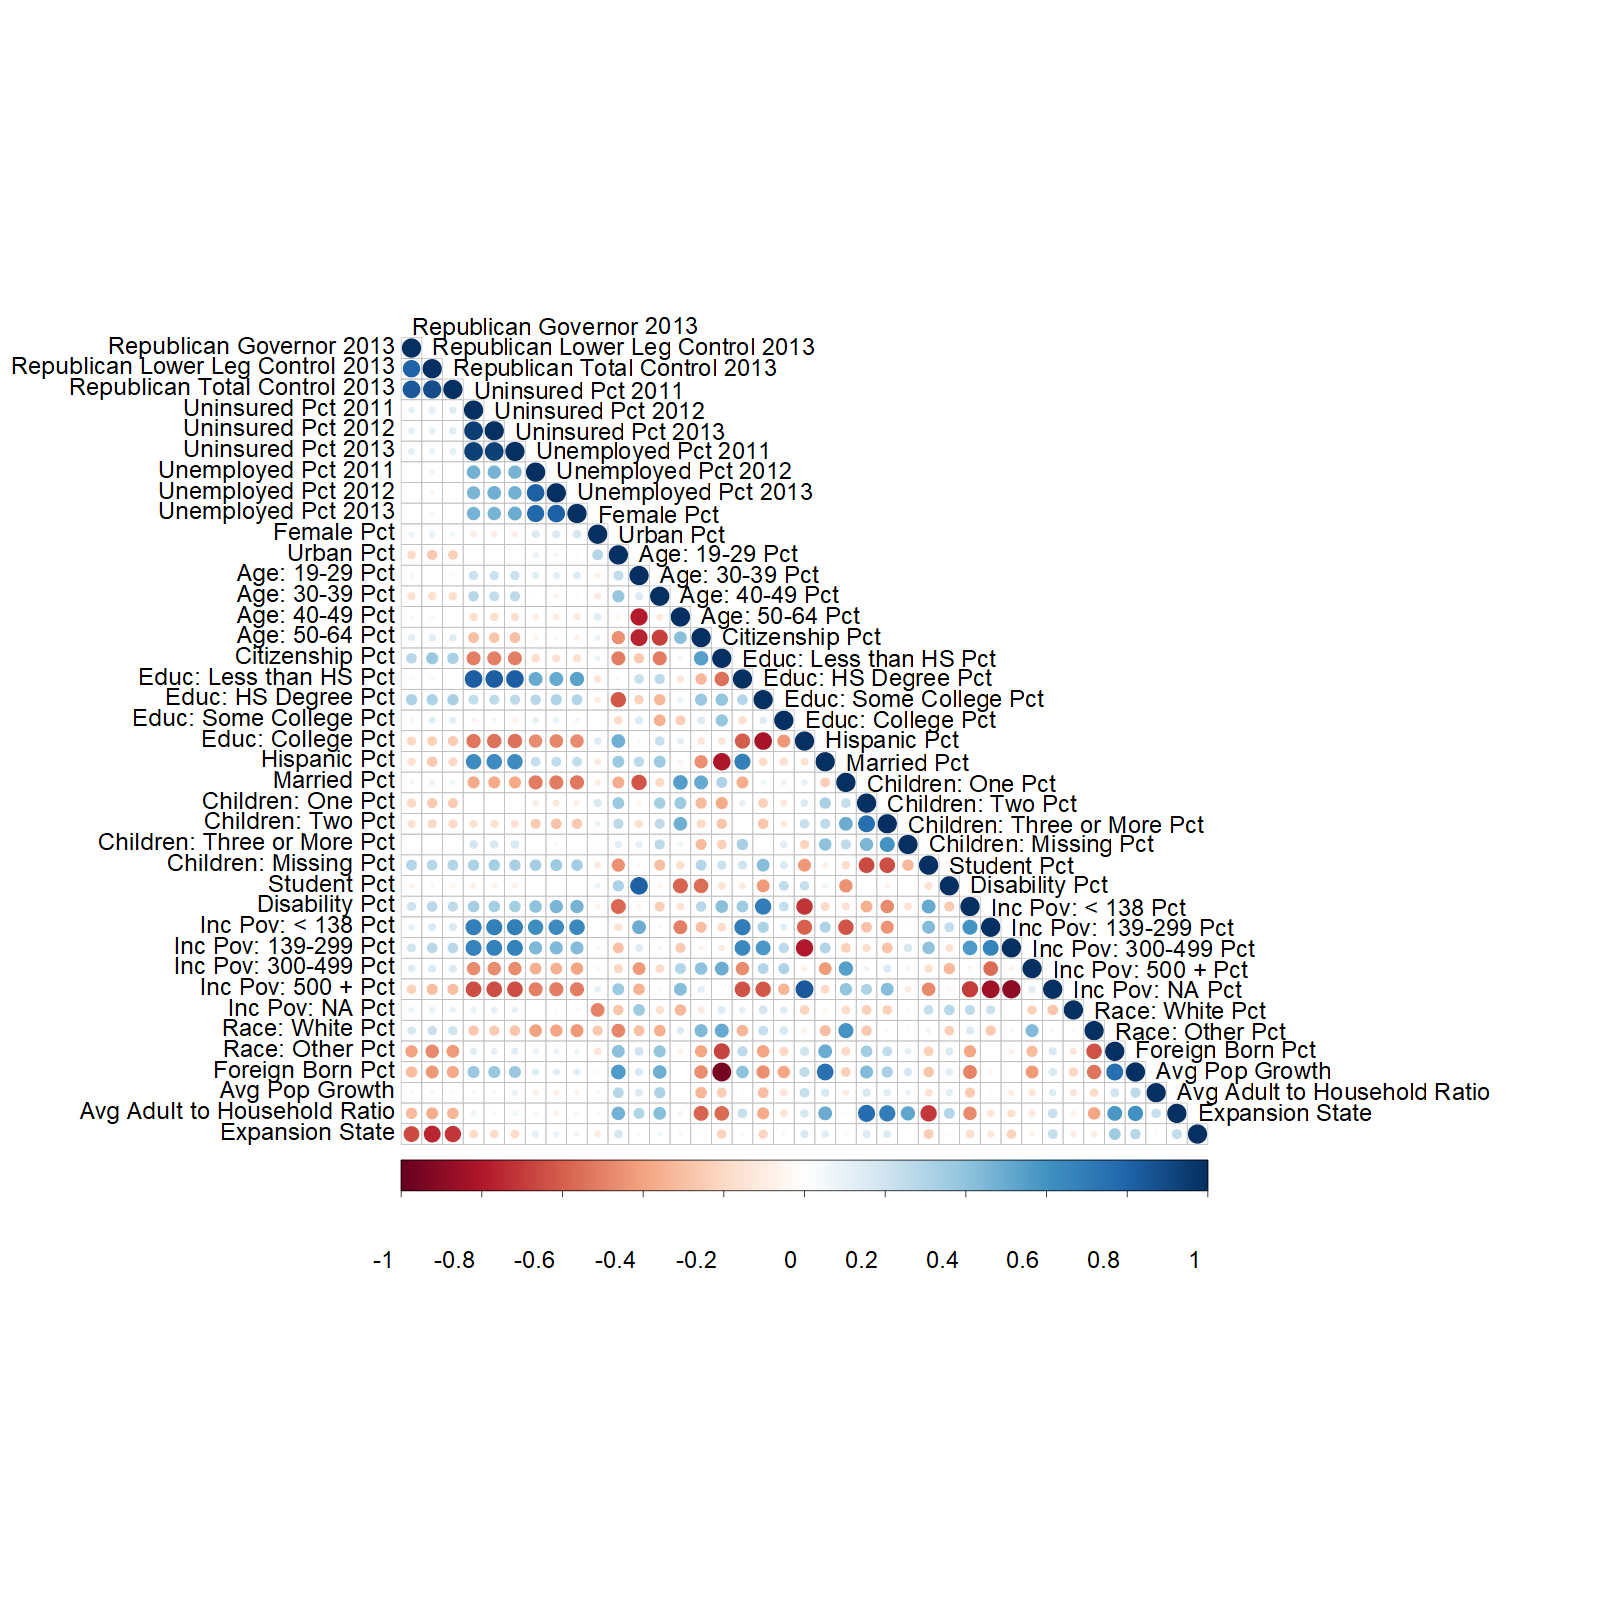
\includegraphics[scale=0.25]{01_Plots/correlation-plot-c1-sigma-zero.png}
\end{center}
\end{figure}

\clearpage

\begin{landscape}

\section{Weight Diagnostics}
\label{ssec:balancetables}

Table~\ref{tab:baltab1} displays the differences between the weighted mean covariate values of the expansion region and the mean of the non-expansion region for our primary dataset and with the early expansion states excluded (calculated using our the homogeneous covariate adjustments). The weights presented here are for the H-SBW estimator. The values under each column are in the following format: (unweighted difference, weighted difference). ``Primary'' and ``Early excluded'' refer to the primary dataset and those that exclude the early expansion states. ``Percent'' indicates that the differences displayed are in percentage points while ``Standardized'' indicates that the standardized mean differences are displayed. Additional results are available on request.

\begin{table}[h!]
\centering
    \caption{Balance table: percent and standardized mean differences, H-SBW weights}
    \label{tab:baltab1}
\begin{tabular}{lllll}
  \hline
Variables & Preferred (Percent) & Preferred (Standardized) & Early excluded (Percent) & Early excluded (Standardized) \\ 
  \hline
Age: 19-29 Pct & (-0.34, -0.34) & (-0.05, -0.05) & (-0.62, -0.21) & (-0.09, -0.03) \\ 
  Age: 30-39 Pct & (0.36, 0.17) & (0.1, 0.05) & (-0.04, 0.32) & (-0.01, 0.09) \\ 
  Age: 40-49 Pct & (0.19, -0.3) & (0.06, -0.1) & (-0.01, -0.44) & (0, -0.15) \\ 
  Avg Adult to Household Ratio & (11.29, -0.04) & (0.37, 0) & (3.37, 0.1) & (0.13, 0) \\ 
  Citizenship Pct & (-3.61, -1.59) & (-0.33, -0.15) & (-0.24, -1.45) & (-0.03, -0.16) \\ 
  Disability Pct & (-1.45, 0.52) & (-0.27, 0.1) & (-0.17, 0.63) & (-0.03, 0.11) \\ 
  Educ: HS Degree Pct & (-3.37, 0.54) & (-0.32, 0.05) & (-1.02, 0.64) & (-0.1, 0.06) \\ 
  Educ: Less than HS Pct & (-0.37, 0.83) & (-0.04, 0.1) & (-1.22, 0.76) & (-0.16, 0.1) \\ 
  Educ: Some College Pct & (-0.35, 0.4) & (-0.05, 0.06) & (0.36, 0.57) & (0.05, 0.08) \\ 
  Female Pct & (-0.34, -0.64) & (-0.16, -0.3) & (-0.25, -1) & (-0.12, -0.48) \\ 
  Foreign Born Pct & (7.6, 2) & (0.42, 0.11) & (1.02, 2) & (0.07, 0.13) \\ 
  Uninsured Pct 2011 & (-3.08, 0.05) & (-0.28, 0) & (-3.51, -0.05) & (-0.34, 0) \\ 
  Uninsured Pct 2012 & (-3, -0.05) & (-0.27, 0) & (-3.4, 0.05) & (-0.33, 0) \\ 
  Uninsured Pct 2013 & (-2.99, -0.05) & (-0.27, 0) & (-3.45, -0.05) & (-0.34, 0) \\ 
  Hispanic Pct & (4.46, 1) & (0.2, 0.04) & (-1.35, 1) & (-0.07, 0.05) \\ 
  Inc Pov: $<$ 138 Pct & (-2.05, 0.63) & (-0.19, 0.06) & (-1.33, 0.12) & (-0.12, 0.01) \\ 
  Inc Pov: 139-299 Pct & (-2.45, 0.65) & (-0.35, 0.09) & (-1.53, 0.5) & (-0.23, 0.08) \\ 
  Inc Pov: 300-499 Pct & (-0.59, -0.18) & (-0.12, -0.04) & (0.28, -0.18) & (0.06, -0.04) \\ 
  Inc Pov: 500 + Pct & (5.58, -1.3) & (0.35, -0.08) & (2.9, -1.23) & (0.2, -0.08) \\ 
  Married Pct & (-0.76, -0.43) & (-0.07, -0.04) & (-0.21, -0.53) & (-0.02, -0.05) \\ 
  Children: Missing Pct & (-3.25, -1) & (-0.36, -0.11) & (-1.99, -0.1) & (-0.21, -0.01) \\ 
  Children: One Pct & (0.7, -0.14) & (0.25, -0.05) & (0.11, -0.31) & (0.04, -0.12) \\ 
  Avg Pop Growth & (-0.09, -0.21) & (-0.07, -0.18) & (-0.26, -0.19) & (-0.22, -0.16) \\ 
  Race: White Pct & (-4.02, 1) & (-0.16, 0.04) & (0.09, 1) & (0, 0.04) \\ 
  Republican Governor 2013 & (-64.78, -25) & (-1.28, -0.5) & (-54.46, -24.87) & (-1.02, -0.47) \\ 
  Republican Lower Leg Control 2013 & (-74.72, -25) & (-1.69, -0.57) & (-56.67, -23.6) & (-1.12, -0.47) \\ 
  Republican Total Control 2013 & (-71.3, -25) & (-1.45, -0.51) & (-56.47, -25) & (-1.02, -0.45) \\ 
  Student Pct & (0.25, -0.5) & (0.04, -0.08) & (0.11, -0.25) & (0.02, -0.04) \\ 
  Children: Three or More Pct & (0, -0.21) & (0, -0.08) & (-0.17, -0.26) & (-0.07, -0.11) \\ 
  Children: Two Pct & (0.76, -0.31) & (0.23, -0.09) & (0.17, -0.37) & (0.05, -0.12) \\ 
  Unemployed Pct 2011 & (0.82, 0.15) & (0.18, 0.03) & (0.68, 0.15) & (0.15, 0.03) \\ 
  Unemployed Pct 2012 & (0.63, -0.03) & (0.14, -0.01) & (0.47, -0.03) & (0.11, -0.01) \\ 
  Unemployed Pct 2013 & (0.42, -0.15) & (0.11, -0.04) & (0.22, -0.15) & (0.06, -0.04) \\ 
  Urban Pct & (8.28, -2) & (0.26, -0.06) & (2.79, -2) & (0.08, -0.06) \\ 
   \hline
\end{tabular}
    \begin{tablenotes}
      \small
      \item The values displayed in each cell are the (weighted, unweighted) differences. The columns containing ``Standardized'' reflect the standardized mean differences while ``percent'' indicates the mean differences in percentage points. The columns containing ``Preferred'' indicate that this is for our primary analysis while ``Early excluded'' is for our analysis that excludes the early expansion states.
    \end{tablenotes}
\end{table}

Figure~\ref{fig:weightsbystatec2} display the weights summed by states when excluding the early expansion states for the H-SBW and BC-HSBW estimators.

\begin{figure}[H]
\begin{center}
    \caption{Total weights summed by state, early expansion removed}
    \label{fig:weightsbystatec2}
    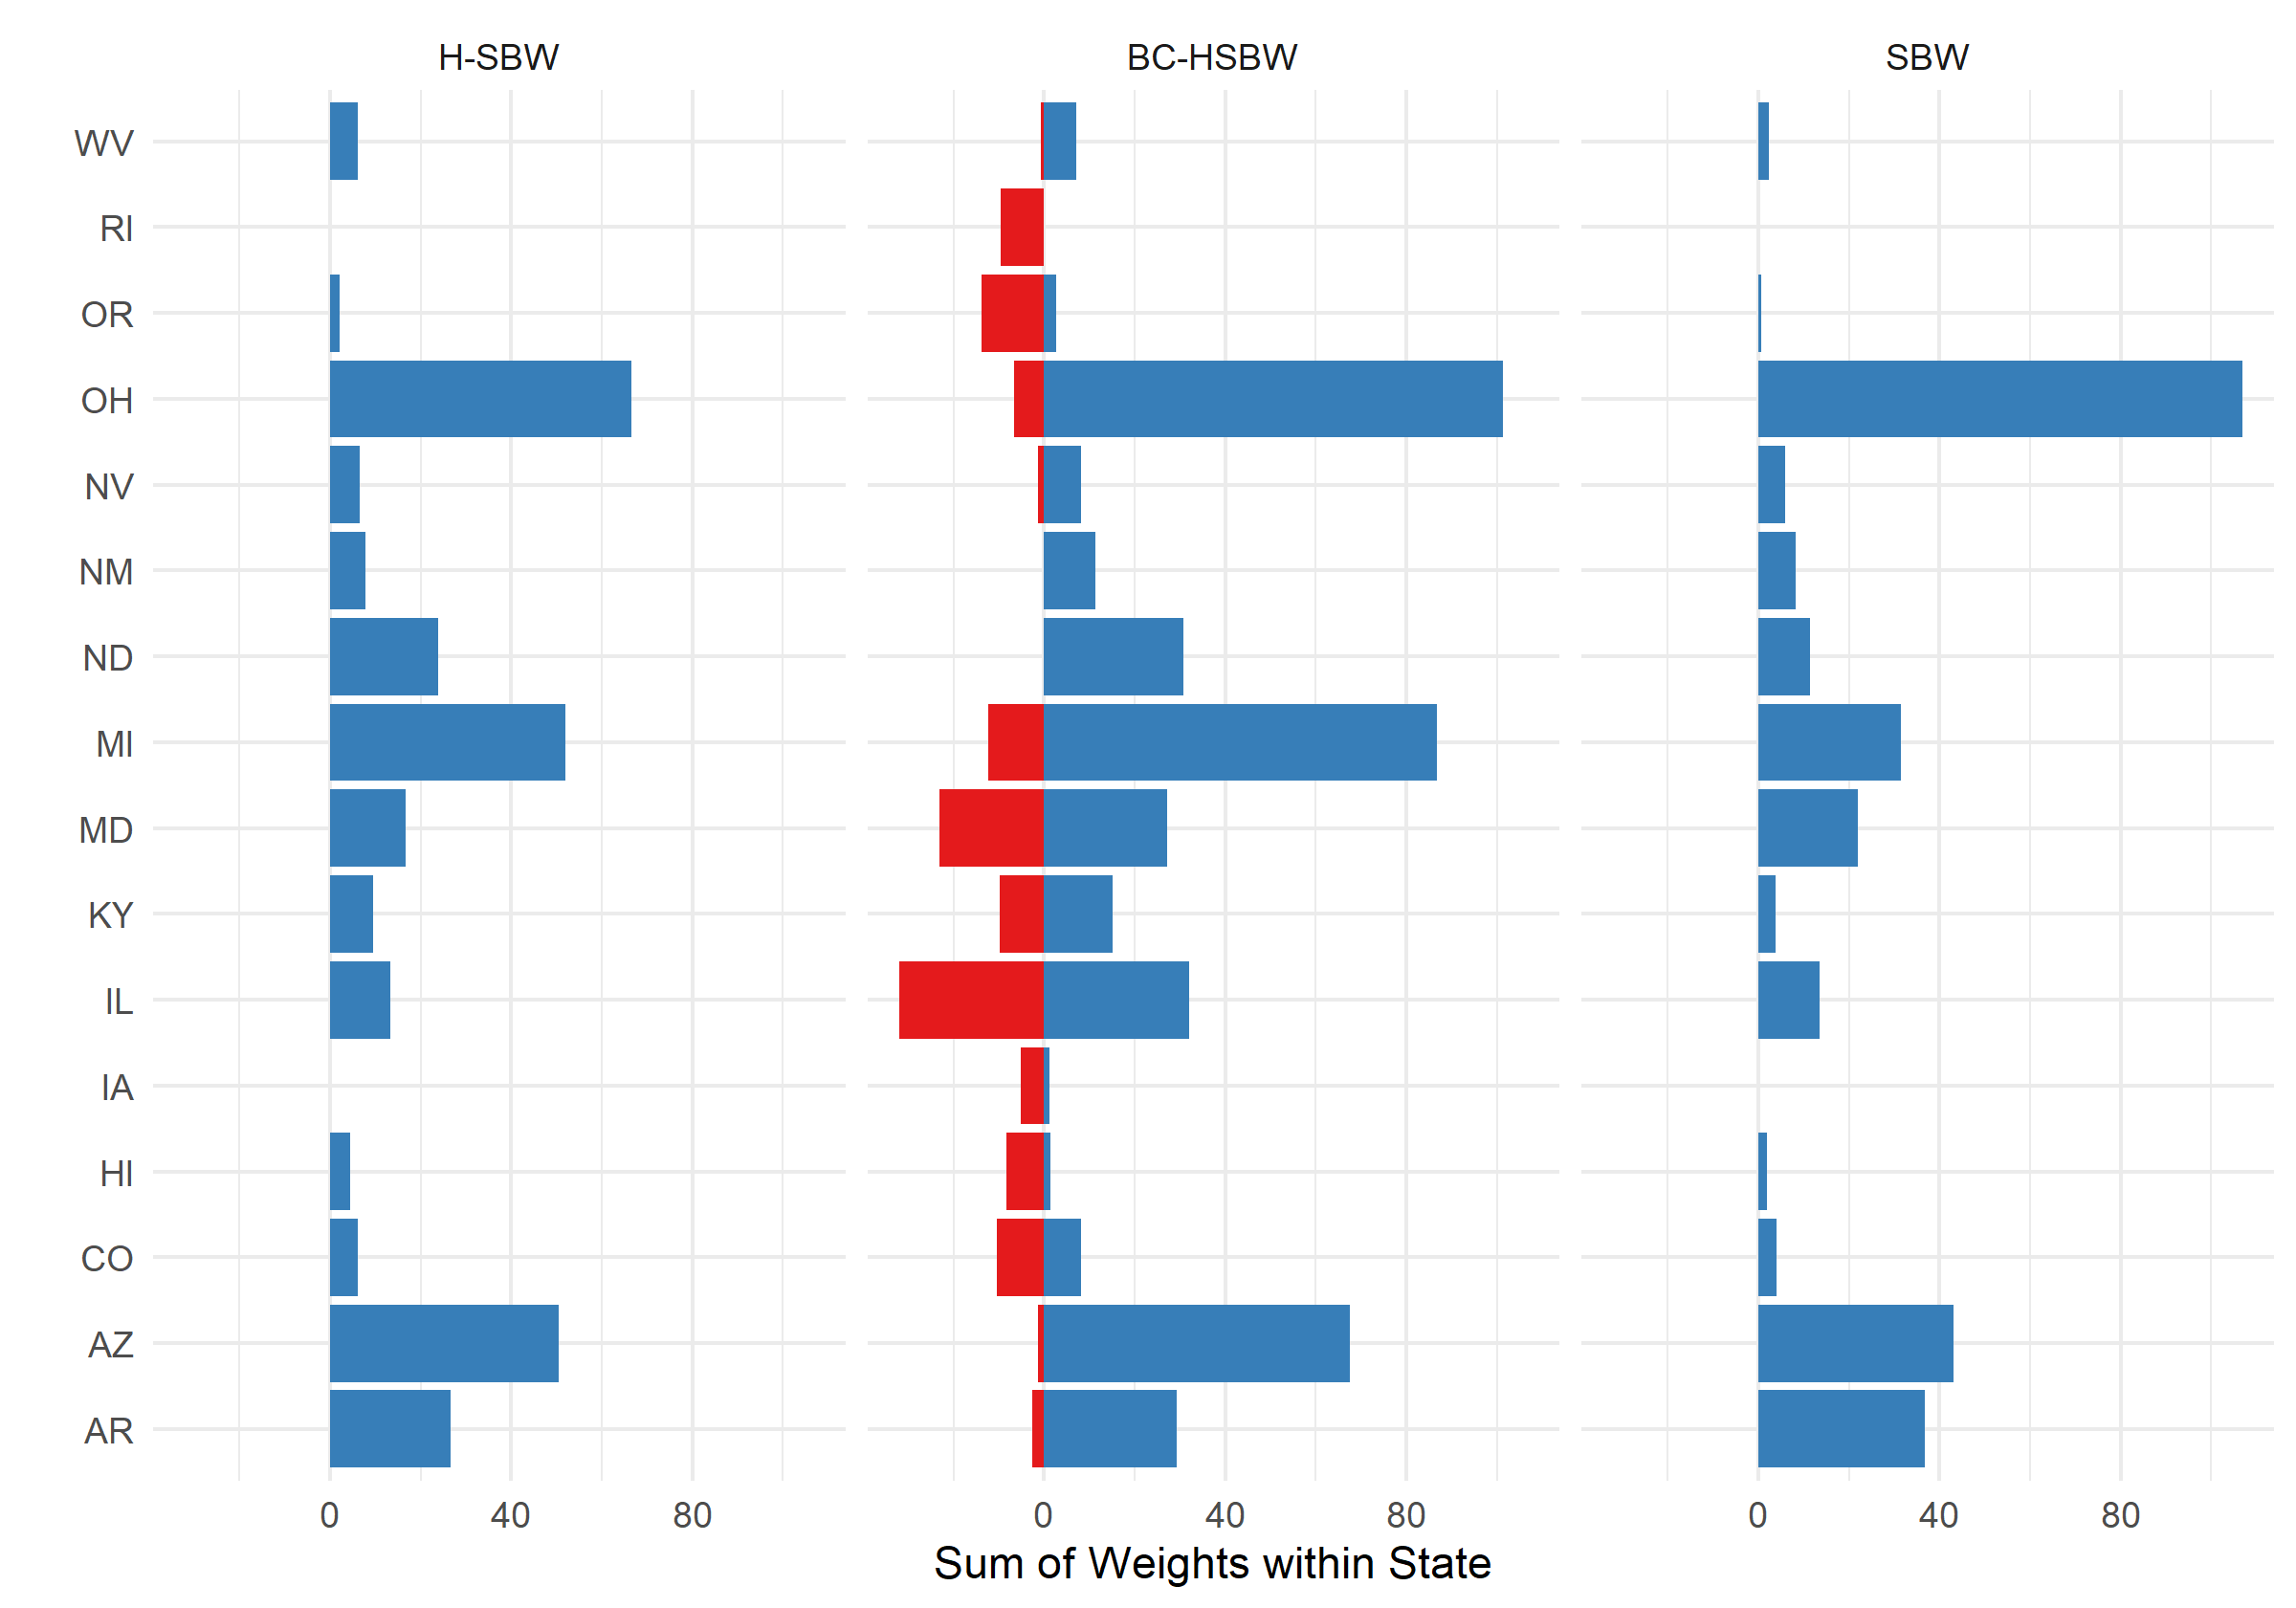
\includegraphics[scale=0.5]{01_Plots/weights-by-state-sbw-hsbw-c2-color.png}
\end{center}
\end{figure}
\end{landscape}
\clearpage

\section{Additional Results}
\label{ssec:allresults}

Table~\ref{tab:confintmain} displays the point estimates from all estimators as well as confidence intervals calculated either (a) leave-one-state-out jackknife on the adjusted dataset (CI (states)); (b) leave-one-state-out jackknife repeating the entire adjusted leaving each state out (CI (proc)). This table also includes all analyses calculated on a second version of the adjusted data where we use a common $\kappa$ for all values (sigma\_uu\_avg), which is the adjustment suggested by \cite{carroll2006measurement}. Notice that the confidence intervals are identical for ``sigma\_zero'' because this is the unadjusted dataset. ``sigma\_uu\_i'' is our preferred covariate adjustment.

\begin{table}[ht]
\centering
\caption{Point estimates and confidence intervals, primary dataset}
\label{tab:confintmain}
\begin{tabular}{llrll}
  \hline
Weight type & Sigma estimate & Psihat & CI (states) & CI (proc) \\ 
  \hline
H-SBW & sigma\_uu\_i & -2.17 & (-3.41, -0.94) & (-3.42, -0.92) \\ 
  H-SBW & sigma\_uu\_avg & -2.25 & (-3.51, -0.99) & (-3.35, -1.14) \\ 
  H-SBW & sigma\_zero & -2.35 & (-3.09, -1.61) & (-3.09, -1.61) \\ 
  BC-HSBW & sigma\_uu\_i & -2.13 & (-3.55, -0.71) & (-3.42, -0.84) \\ 
  BC-HSBW & sigma\_uu\_avg & -2.17 & (-3.57, -0.78) & (-3.39, -0.96) \\ 
  BC-HSBW & sigma\_zero & -2.40 & (-3.33, -1.46) & (-3.33, -1.46) \\ 
  SBW & sigma\_uu\_i & -2.24 & (-3.50, -0.99) & (-3.51, -0.97) \\ 
  SBW & sigma\_uu\_avg & -2.30 & (-3.67, -0.92) & (-3.45, -1.15) \\ 
  SBW & sigma\_zero & -2.40 & (-3.10, -1.69) & (-3.10, -1.69) \\ 
  BC-SBW & sigma\_uu\_i & -2.12 & (-3.15, -1.10) & (-3.11, -1.14) \\ 
  BC-SBW & sigma\_uu\_avg & -2.17 & (-3.25, -1.08) & (-3.22, -1.12) \\ 
  BC-SBW & sigma\_zero & -2.36 & (-2.93, -1.80) & (-2.93, -1.80) \\ 
   \hline
\end{tabular}
\end{table}

Table~\ref{tab:ptests} presents all point estimates from estimators that we calculated. The ``Var subset`` column indicates which variables were excluded from the estimation: 0 excludes no variables; 1 removes Republican governance indicators; 2 pre-treatment uninsurance and unemployment rates; 3 urban, age, education, citizenship, marital status, student, disability, or female; 4 race, ethnicity, income, foreign born; 5 children, population growth, and household to person ratio. We see that the largest changes generally occur when excluding the pre-treatment uninsurance and unemployment rates. This is not surprising: controlling for the other covariates, the pre-treatment uninsurance rate was substantially lower in the treated region compared to the control region. Given that pre-treatment uninsurance rates are highly correlated with post-treatment rates, we find that this comparison leads to a larger absolute magnitude point estimate, highlighting the need to control for these covariates.

%Wed Jan 13 15:24:43 2021
\begin{table}[ht]
\centering
\caption{Point estimates for all specifications}
\label{tab:ptests}
\begin{tabular}{rlrrrr}
  \hline
Variable subset & Sigma estimate & H-SBW & BC-HSBW & SBW & BC-SBW \\ 
  \hline
0 & sigma\_uu\_i & -2.17 & -2.13 & -2.24 & -2.12 \\ 
  0 & sigma\_uu\_avg & -2.25 & -2.17 & -2.30 & -2.17 \\ 
  0 & sigma\_zero & -2.35 & -2.40 & -2.40 & -2.36 \\ 
  1 & sigma\_uu\_i & -2.85 & -2.87 & -3.00 & -2.76 \\ 
  1 & sigma\_uu\_avg & -2.86 & -2.86 & -2.99 & -2.75 \\ 
  1 & sigma\_zero & -3.00 & -3.09 & -3.07 & -2.92 \\ 
  2 & sigma\_uu\_i & -5.73 & -5.05 & -5.24 & -4.70 \\ 
  2 & sigma\_uu\_avg & -5.73 & -5.05 & -5.24 & -4.70 \\ 
  2 & sigma\_zero & -5.73 & -5.13 & -5.24 & -4.77 \\ 
  3 & sigma\_uu\_i & -2.17 & -2.00 & -2.24 & -2.00 \\ 
  3 & sigma\_uu\_avg & -2.25 & -2.06 & -2.29 & -2.06 \\ 
  3 & sigma\_zero & -2.34 & -2.17 & -2.40 & -2.15 \\ 
  4 & sigma\_uu\_i & -2.35 & -2.39 & -2.29 & -2.30 \\ 
  4 & sigma\_uu\_avg & -2.39 & -2.39 & -2.32 & -2.32 \\ 
  4 & sigma\_zero & -2.45 & -2.59 & -2.43 & -2.49 \\ 
  5 & sigma\_uu\_i & -2.17 & -2.19 & -2.26 & -2.21 \\ 
  5 & sigma\_uu\_avg & -2.25 & -2.24 & -2.33 & -2.27 \\ 
  5 & sigma\_zero & -2.35 & -2.44 & -2.42 & -2.47 \\ 
   \hline
\end{tabular}
\end{table}

Table ~\ref{tab:confintmainc2} and Table~\ref{tab:secondaryptests} are identical to the structure of the previous two tables except we exclude the ``early expansion states'' from the pool of expansion state matches. 

\begin{table}[ht]
\centering
\caption{Point estimates and confidence intervals, early expansion excluded}
\label{tab:confintmainc2}
\begin{tabular}{llrll}
  \hline
Weight type & Sigma estimate & Psihat & CI (states) & CI (proc) \\ 
  \hline
H-SBW & sigma\_uu\_i & -2.05 & (-3.10, -1.00) & (-3.05, -1.05) \\ 
  H-SBW & sigma\_uu\_avg & -2.13 & (-3.20, -1.05) & (-3.17, -1.08) \\ 
  H-SBW & sigma\_zero & -2.29 & (-2.90, -1.69) & (-2.90, -1.69) \\ 
  BC-HSBW & sigma\_uu\_i & -2.14 & (-3.63, -0.64) & (-3.48, -0.80) \\ 
  BC-HSBW & sigma\_uu\_avg & -2.19 & (-3.65, -0.73) & (-3.57, -0.81) \\ 
  BC-HSBW & sigma\_zero & -2.50 & (-3.66, -1.33) & (-3.66, -1.33) \\ 
  SBW & sigma\_uu\_i & -1.91 & (-2.91, -0.91) & (-2.79, -1.03) \\ 
  SBW & sigma\_uu\_avg & -2.01 & (-3.02, -1.00) & (-2.83, -1.19) \\ 
  SBW & sigma\_zero & -2.20 & (-2.69, -1.71) & (-2.69, -1.71) \\ 
  BC-SBW & sigma\_uu\_i & -1.97 & (-3.49, -0.44) & (-3.27, -0.66) \\ 
  BC-SBW & sigma\_uu\_avg & -2.04 & (-3.59, -0.50) & (-3.39, -0.70) \\ 
  BC-SBW & sigma\_zero & -2.34 & (-3.44, -1.25) & (-3.44, -1.25) \\ 
   \hline
\end{tabular}
\end{table}

\begin{table}[ht]
\centering
   \caption{Point estimates for all specifications, early expansion excluded}
    \label{tab:secondaryptests}
\begin{tabular}{rlrrrr}
  \hline
Variable subset & Sigma estimate & H-SBW & BC-HSBW & SBW & BC-SBW \\ 
  \hline
0 & sigma\_uu\_i & -2.05 & -2.14 & -1.91 & -1.97 \\ 
  0 & sigma\_uu\_avg & -2.13 & -2.19 & -2.01 & -2.04 \\ 
  0 & sigma\_zero & -2.29 & -2.50 & -2.20 & -2.34 \\ 
  1 & sigma\_uu\_i & -2.85 & -2.99 & -2.85 & -2.86 \\ 
  1 & sigma\_uu\_avg & -2.86 & -2.98 & -2.86 & -2.86 \\ 
  1 & sigma\_zero & -3.05 & -3.18 & -2.96 & -2.99 \\ 
  2 & sigma\_uu\_i & -5.55 & -4.46 & -5.02 & -4.52 \\ 
  2 & sigma\_uu\_avg & -5.55 & -4.73 & -5.01 & -4.53 \\ 
  2 & sigma\_zero & -5.55 & -4.78 & -5.01 & -4.56 \\ 
  3 & sigma\_uu\_i & -2.05 & -2.03 & -1.91 & -1.89 \\ 
  3 & sigma\_uu\_avg & -2.13 & -2.10 & -2.00 & -1.97 \\ 
  3 & sigma\_zero & -2.27 & -2.22 & -2.20 & -2.13 \\ 
  4 & sigma\_uu\_i & -2.27 & -2.24 & -2.15 & -2.00 \\ 
  4 & sigma\_uu\_avg & -2.35 & -2.28 & -2.23 & -2.04 \\ 
  4 & sigma\_zero & -2.36 & -2.62 & -2.28 & -2.45 \\ 
  5 & sigma\_uu\_i & -2.05 & -2.20 & -1.91 & -2.03 \\ 
  5 & sigma\_uu\_avg & -2.13 & -2.26 & -1.99 & -2.11 \\ 
  5 & sigma\_zero & -2.29 & -2.45 & -2.19 & -2.36 \\ 
   \hline
\end{tabular}
\end{table}

Table~\ref{tab:loostatec1} and Table~\ref{tab:loostatec2} present point estimates for the leave-one-state out analysis for our preferred estimator, H-SBW calculated on our preferred covariate adjustment for the primary dataset and when excluding early expansion states.

\begin{table}[ht]
\centering
   \caption{Leave-one-state-out point estimates, primary dataset, preferred adjustment}
    \label{tab:loostatec1}
\begin{tabular}{lrlrl}
  \hline
State & Psihat (0) & None (states, proc) & Psihat (1) & Repub (states, proc) \\ 
  \hline
AR & -2.17 & (-2.34, -2.38) & -2.85 & (-2.81, -2.80) \\ 
  AZ & -2.17 & (-2.21, -2.24) & -2.85 & (-2.86, -2.86) \\ 
  CA & -2.17 & (-1.99, -2.02) & -2.85 & (-2.77, -2.76) \\ 
  CO & -2.17 & (-2.17, -2.23) & -2.85 & (-2.84, -2.84) \\ 
  CT & -2.17 & (-2.17, -2.15) & -2.85 & (-2.83, -2.82) \\ 
  HI & -2.17 & (-2.15, -2.14) & -2.85 & (-2.77, -2.78) \\ 
  IA & -2.17 & (-2.09, -2.07) & -2.85 & (-2.83, -2.84) \\ 
  IL & -2.17 & (-2.16, -2.24) & -2.85 & (-2.83, -2.84) \\ 
  KY & -2.17 & (-2.02, -1.95) & -2.85 & (-2.57, -2.52) \\ 
  MD & -2.17 & (-2.25, -2.27) & -2.85 & (-2.94, -2.94) \\ 
  MI & -2.17 & (-2.10, -2.18) & -2.85 & (-2.89, -2.92) \\ 
  MN & -2.17 & (-2.17, -2.19) & -2.85 & (-2.84, -2.86) \\ 
  ND & -2.17 & (-2.23, -2.26) & -2.85 & (-2.84, -2.84) \\ 
  NH & -2.17 & (-2.18, -2.21) & -2.85 & (-2.98, -2.99) \\ 
  NJ & -2.17 & (-2.26, -2.25) & -2.85 & (-2.99, -3.03) \\ 
  NM & -2.17 & (-2.16, -2.22) & -2.85 & (-2.76, -2.77) \\ 
  NV & -2.17 & (-2.21, -2.24) & -2.85 & (-2.89, -2.88) \\ 
  OH & -2.17 & (-2.70, -2.68) & -2.85 & (-3.00, -2.98) \\ 
  OR & -2.17 & (-2.17, -2.25) & -2.85 & (-2.80, -2.84) \\ 
  RI & -2.17 & (-2.17, -2.15) & -2.85 & (-2.81, -2.81) \\ 
  WA & -2.17 & (-2.10, -2.11) & -2.85 & (-2.78, -2.77) \\ 
  WV & -2.17 & (-2.16, -2.18) & -2.85 & (-2.8, -2.78) \\ 
   \hline
\end{tabular}
\end{table}

\begin{table}[ht]
\centering
   \caption{Leave-one-state-out point estimates, early expansion excluded, preferred adjustment}
    \label{tab:loostatec2}
\begin{tabular}{lrlrl}
  \hline
State & Psihat (0) & None (states, proc) & Psihat (1) & Repub (states, proc) \\ 
  \hline
AR & -2.05 & (-2.15, -2.16) & -2.85 & (-2.77, -2.76) \\ 
  AZ & -2.05 & (-1.82, -1.88) & -2.85 & (-2.87, -2.86) \\ 
  CO & -2.05 & (-2.07, -2.09) & -2.85 & (-2.84, -2.83) \\ 
  HI & -2.05 & (-2.01, -1.99) & -2.85 & (-2.71, -2.73) \\ 
  IA & -2.05 & (-1.98, -1.95) & -2.85 & (-2.85, -2.86) \\ 
  IL & -2.05 & (-2.03, -2.01) & -2.85 & (-2.8, -2.79) \\ 
  KY & -2.05 & (-1.87, -1.8) & -2.85 & (-2.59, -2.54) \\ 
  MD & -2.05 & (-2.18, -2.15) & -2.85 & (-2.97, -2.96) \\ 
  MI & -2.05 & (-1.96, -2) & -2.85 & (-2.92, -2.96) \\ 
  ND & -2.05 & (-2.02, -2.04) & -2.85 & (-2.84, -2.84) \\ 
  NH & -2.05 & (-2.05, -2.06) & -2.85 & (-3.02, -3.03) \\ 
  NM & -2.05 & (-1.99, -1.97) & -2.85 & (-2.72, -2.75) \\ 
  NV & -2.05 & (-2.15, -2.15) & -2.85 & (-2.93, -2.92) \\ 
  OH & -2.05 & (-2.43, -2.38) & -2.85 & (-3.03, -3.02) \\ 
  OR & -2.05 & (-2.05, -2.11) & -2.85 & (-2.81, -2.84) \\ 
  RI & -2.05 & (-2.05, -2.05) & -2.85 & (-2.80, -2.80) \\ 
  WV & -2.05 & (-2.06, -2.06) & -2.85 & (-2.83, -2.81) \\ 
   \hline
\end{tabular}
\end{table}

Table~\ref{tab:oateconfint} displays point estimates and confidence intervals for the primary point estimates for the OATE. We display the confidence intervals calculated using both the leave-one-out-states conditional on the covariate adjustment (CI (states)) and recalculating the covariate adjustment for the OATE (CI (proc)). 

\begin{table}[ht]
\centering
\caption{OATE primary results inference}
\label{tab:oateconfint}
\begin{tabular}{rllll}
  \hline
Psihat & Sigma estimate & Dataset & CI (states) & CI (proc) \\ 
  \hline
-1.74 & sigma\_uu\_i\_modeled & c1 & (-2.35, -1.14) & (-2.48, -1.00) \\ 
  -1.67 & sigma\_uu\_avg & c1 & (-2.34, -0.99) & (-2.52, -0.81) \\ 
  -1.80 & sigma\_zero & c1 & (-2.50, -1.10) & (-2.50, -1.10) \\ 
  -1.89 & sigma\_uu\_i\_modeled & c2 & (-2.47, -1.32) & (-2.54, -1.24) \\ 
  -1.80 & sigma\_uu\_avg & c2 & (-2.43, -1.17) & (-2.57, -1.03) \\ 
  -1.95 & sigma\_zero & c2 & (-2.65, -1.25) & (-2.65, -1.25) \\ 
   \hline
\end{tabular}
\end{table}

Table~\ref{tab:oatesensitive} presents all point estimates calculate using the overlap weights. Dataset ``c1'' refers to the primary dataset and dataset ``c2'' removes the early expansion states. The numeric column names refer to the covariate group excluded (covariate groups described above).

\begin{table}[ht]
\centering
\caption{OATE all point estimates}
\label{tab:oatesensitive}
\begin{tabular}{llrrrrrr}
  \hline
Sigma estimate & Dataset & 0 & 1 & 2 & 3 & 4 & 5 \\ 
  \hline
sigma\_uu\_i & c1 & -1.64 & -2.60 & -2.96 & -1.86 & -1.86 & -1.77 \\ 
  sigma\_uu\_i & c2 & -1.81 & -2.53 & -3.10 & -2.18 & -2.04 & -1.96 \\ 
  sigma\_avg & c1 & -1.58 & -2.62 & -2.85 & -1.76 & -1.76 & -1.78 \\ 
  sigma\_avg & c2 & -1.74 & -2.54 & -3.00 & -2.10 & -1.96 & -1.95 \\ 
  sigma\_zero & c1 & -1.80 & -2.55 & -3.11 & -1.98 & -1.94 & -1.83 \\ 
  sigma\_zero & c2 & -1.95 & -2.51 & -3.25 & -2.12 & -2.10 & -2.00 \\ 
   \hline
\end{tabular}
\end{table}

Table~\ref{tab:rdiffc1} and ~\ref{tab:rdiffc2} display the quantiles of the distribution $\hat{\Delta}_v^1$ estimates when leaving out each state for the primary dataset and removing the early expansion states. The ``resample'' column indicates whether the entire adjustment procedure was recalculated (``proc'') or whether we left out each state conditional on the adjustment (``states''). Table~\ref{tab:hte} displays the estimated linear combination of model coefficients on the Republican governance indicators with 95 percent confidence intervals (standard errors clustered at the state level). The ``Weights'' column represents whether the regressions were weighted; we ran two versions, an unweighted regression and one using the overlap weights.

\begin{table}[ht]
\centering
\label{tab:rdiffc1}
\caption{$\hat{\Delta}^1_v$ leave-one-state-out estimates, primary dataset}
\begin{tabular}{lllrrrrrr}
  \hline
Resample & Sigma estimate & Weight type & Original & 0\% & 25\% & 50\% & 75\% & 100\% \\ 
  \hline
states & sigma\_uu\_i\_modeled & H-SBW & -0.67 & -0.80 & -0.68 & -0.67 & -0.62 & -0.30 \\ 
  proc & sigma\_uu\_i\_modeled & H-SBW & -0.67 & -0.78 & -0.68 & -0.64 & -0.59 & -0.30 \\ 
  states & sigma\_uu\_i\_modeled & BC-HSBW & -0.74 & -0.87 & -0.77 & -0.71 & -0.69 & -0.26 \\ 
  proc & sigma\_uu\_i\_modeled & BC-HSBW & -0.74 & -0.85 & -0.76 & -0.70 & -0.67 & -0.34 \\ 
  states & sigma\_uu\_i\_modeled & SBW & -0.75 & -0.98 & -0.77 & -0.75 & -0.72 & -0.48 \\ 
  proc & sigma\_uu\_i\_modeled & SBW & -0.75 & -0.98 & -0.78 & -0.73 & -0.67 & -0.49 \\ 
  states & sigma\_uu\_i\_modeled & BC-SBW & -0.63 & -0.85 & -0.69 & -0.62 & -0.61 & -0.39 \\ 
  proc & sigma\_uu\_i\_modeled & BC-SBW & -0.63 & -0.82 & -0.68 & -0.64 & -0.59 & -0.35 \\ 
  states & sigma\_uu\_avg & H-SBW & -0.61 & -0.74 & -0.64 & -0.60 & -0.57 & -0.23 \\ 
  proc & sigma\_uu\_avg & H-SBW & -0.61 & -0.76 & -0.63 & -0.59 & -0.55 & -0.33 \\ 
  states & sigma\_uu\_avg & BC-HSBW & -0.69 & -0.83 & -0.73 & -0.68 & -0.64 & -0.24 \\ 
  proc & sigma\_uu\_avg & BC-HSBW & -0.69 & -0.83 & -0.73 & -0.66 & -0.63 & -0.39 \\ 
  states & sigma\_uu\_avg & SBW & -0.70 & -0.89 & -0.72 & -0.69 & -0.67 & -0.31 \\ 
  proc & sigma\_uu\_avg & SBW & -0.70 & -0.93 & -0.73 & -0.68 & -0.65 & -0.49 \\ 
  states & sigma\_uu\_avg & BC-SBW & -0.58 & -0.78 & -0.63 & -0.57 & -0.56 & -0.32 \\ 
  proc & sigma\_uu\_avg & BC-SBW & -0.58 & -0.81 & -0.63 & -0.58 & -0.55 & -0.28 \\ 
  states & sigma\_zero & H-SBW & -0.65 & -0.78 & -0.66 & -0.63 & -0.61 & -0.50 \\ 
  proc & sigma\_zero & H-SBW & -0.65 & -0.78 & -0.66 & -0.63 & -0.61 & -0.50 \\ 
  states & sigma\_zero & BC-HSBW & -0.70 & -0.88 & -0.74 & -0.68 & -0.64 & -0.50 \\ 
  proc & sigma\_zero & BC-HSBW & -0.70 & -0.88 & -0.74 & -0.68 & -0.64 & -0.50 \\ 
  states & sigma\_zero & SBW & -0.68 & -0.84 & -0.71 & -0.68 & -0.66 & -0.49 \\ 
  proc & sigma\_zero & SBW & -0.68 & -0.84 & -0.71 & -0.68 & -0.66 & -0.49 \\ 
  states & sigma\_zero & BC-SBW & -0.56 & -0.67 & -0.61 & -0.55 & -0.52 & -0.39 \\ 
  proc & sigma\_zero & BC-SBW & -0.56 & -0.67 & -0.61 & -0.55 & -0.52 & -0.39 \\ 
   \hline
\end{tabular}
\end{table}

\begin{table}[ht]
\label{tab:rdiffc2}
\caption{$\hat{\Delta}^1_v$ leave-one-state-out estimates, early expansion excluded}
\centering
\begin{tabular}{lllrrrrrr}
  \hline
Resample & Sigma estimate & Weight type & Original & 0\% & 25\% & 50\% & 75\% & 100\% \\ 
  \hline
states & sigma\_uu\_i\_modeled & H-SBW & -0.80 & -1.05 & -0.82 & -0.77 & -0.73 & -0.60 \\ 
  proc & sigma\_uu\_i\_modeled & H-SBW & -0.80 & -0.98 & -0.81 & -0.76 & -0.74 & -0.60 \\ 
  states & sigma\_uu\_i\_modeled & BC-HSBW & -0.85 & -1.13 & -0.96 & -0.83 & -0.76 & -0.45 \\ 
  proc & sigma\_uu\_i\_modeled & BC-HSBW & -0.85 & -1.05 & -0.94 & -0.83 & -0.77 & -0.53 \\ 
  states & sigma\_uu\_i\_modeled & SBW & -0.94 & -1.15 & -0.94 & -0.92 & -0.89 & -0.70 \\ 
  proc & sigma\_uu\_i\_modeled & SBW & -0.94 & -1.05 & -0.98 & -0.91 & -0.86 & -0.73 \\ 
  states & sigma\_uu\_i\_modeled & BC-SBW & -0.89 & -1.27 & -0.93 & -0.86 & -0.81 & -0.26 \\ 
  proc & sigma\_uu\_i\_modeled & BC-SBW & -0.89 & -1.19 & -0.96 & -0.86 & -0.81 & -0.37 \\ 
  states & sigma\_uu\_avg & H-SBW & -0.73 & -0.99 & -0.74 & -0.70 & -0.68 & -0.51 \\ 
  proc & sigma\_uu\_avg & H-SBW & -0.73 & -0.94 & -0.73 & -0.69 & -0.67 & -0.50 \\ 
  states & sigma\_uu\_avg & BC-HSBW & -0.79 & -1.10 & -0.87 & -0.78 & -0.69 & -0.42 \\ 
  proc & sigma\_uu\_avg & BC-HSBW & -0.79 & -1.01 & -0.89 & -0.73 & -0.69 & -0.46 \\ 
  states & sigma\_uu\_avg & SBW & -0.85 & -1.08 & -0.85 & -0.83 & -0.81 & -0.66 \\ 
  proc & sigma\_uu\_avg & SBW & -0.85 & -0.95 & -0.86 & -0.82 & -0.80 & -0.68 \\ 
  states & sigma\_uu\_avg & BC-SBW & -0.82 & -1.21 & -0.86 & -0.80 & -0.74 & -0.18 \\ 
  proc & sigma\_uu\_avg & BC-SBW & -0.82 & -1.09 & -0.86 & -0.76 & -0.74 & -0.26 \\ 
  states & sigma\_zero & H-SBW & -0.76 & -0.95 & -0.83 & -0.74 & -0.70 & -0.58 \\ 
  proc & sigma\_zero & H-SBW & -0.76 & -0.95 & -0.83 & -0.74 & -0.70 & -0.58 \\ 
  states & sigma\_zero & BC-HSBW & -0.69 & -1.00 & -0.83 & -0.70 & -0.60 & -0.39 \\ 
  proc & sigma\_zero & BC-HSBW & -0.69 & -1.00 & -0.83 & -0.70 & -0.60 & -0.39 \\ 
  states & sigma\_zero & SBW & -0.76 & -0.91 & -0.83 & -0.75 & -0.74 & -0.51 \\ 
  proc & sigma\_zero & SBW & -0.76 & -0.91 & -0.83 & -0.75 & -0.74 & -0.51 \\ 
  states & sigma\_zero & BC-SBW & -0.64 & -1.06 & -0.70 & -0.58 & -0.55 & -0.38 \\ 
  proc & sigma\_zero & BC-SBW & -0.64 & -1.06 & -0.70 & -0.58 & -0.55 & -0.38 \\ 
   \hline
\end{tabular}
\end{table}

\begin{table}[ht]
\caption{OLS HTE estimates}
\label{tab:hte}
\centering
\begin{tabular}{rllll}
  \hline
Estimate & Dataset & Sigma estimate & CI 95 & Weights \\ 
  \hline
  -1.76 & c1 & sigma\_uu\_i\_modeled & (-5.47, 1.94) & Overlap \\ 
  -1.67 & c1 & sigma\_uu\_avg & (-7.18, 3.84) & Overlap \\ 
  -1.97 & c1 & sigma\_zero & (-4.11, 0.17) & Overlap \\ 
  0.51 & c2 & sigma\_uu\_i\_modeled & (-6.00, 7.02) & Overlap \\ 
  -0.17 & c2 & sigma\_uu\_avg & (-8.17, 7.83) & Overlap \\ 
  -1.48 & c2 & sigma\_zero & (-3.51, 0.54) & Overlap \\ 
  0.10 & c1 & sigma\_uu\_i\_modeled & (-1.09, 1.30) & None \\ 
  0.61 & c1 & sigma\_uu\_avg & (-1.82, 3.04) & None \\ 
  -0.12 & c1 & sigma\_zero & (-0.90, 0.66) & None \\ 
  0.37 & c2 & sigma\_uu\_i\_modeled & (-0.9, 1.63) & None \\ 
  0.64 & c2 & sigma\_uu\_avg & (-1.77, 3.04) & None \\ 
  -0.11 & c2 & sigma\_zero & (-0.91, 0.68) & None \\ 
   \hline
\end{tabular}
\end{table}


The synthetic controls approach chooses the $\gamma$ that minimizes the weighted L2-squared distance of the covariates using a diagonal weighting matrix $V$. $V$ is then chosen to minimize the mean-square error of the weighted difference in pre-treatment outcomes. Letting $Z_a$ be the matrix of pre-treatment outcomes for treatment group $A = a$, the synthetic controls algorithm solves the following optimization problem for a fixed $V$:

\begin{align}
\gamma(V) = \arg\min_{\tilde{\gamma}(V^\star)} = (\bar{X}_1 - X_0^T\tilde{\gamma})'V(\bar{X}_1 - X_0^T\tilde{\gamma}) 
\end{align}

This is the ``inner'' optimization. $V^\star$ is then determined in an ``outer'' optimization to minimize the imbalances in the pre-treatment outcomes $Z$:

\begin{align}
    V^\star = \arg\min_V (\bar{Z}_1 - Z_0^T\gamma(V))'(\bar{Z}_1 - Z_0^T\gamma(V))
\end{align}

In applications the covariate matrix $X_a$ may contain some elements of $Z_a$. In cases where $X_a$ contains all pre-treatment outcomes, \cite{kaul2015synthetic} has shown that the predictor weights $V^\star$ will give no weight to auxillary covariates (covariates that are not the pre-treatment outcomes), rendering these irrelevant to the model. 

While in practice $V$ is often learned on the same data as the weights, we consider the case where we use cross-validation to choose $V$, as proposed by \cite{abadie2015comparative}. Assume we can divide our pre-treatment data into a training data from periods $T = 1, ..., T - l - 1$, a validation period from periods $T - l, ..., T - 1$, and a post-treatment period at time $T$. To make this discussion more general, assume that we are evaluating a set of candidate models $\mathcal{M}$ on the validation data (where for the synthetic controls algorithm we can think of this as the set of all possible weighting matrices $V$). Let $\bar{Y}^a_{a', t}$ 
be the mean potential outcome under treatment $A = a$ for treatment group $A = a'$ at time $t$ (where $t$ occurs during the validation period). Let $\hat{\bar{Y}}^a_{a'', t}(m)$ be an estimator of that potential outcome at time $t$ using model $m$, which was trained during the training period using data from treatment group $A = a''$. Finally, let $\bar{Y}_{a'}^{a_T}$ be the post-treatment estimand, where $\hat{Y}^a_{a'', T}(m)$ is the estimator using model $m$ trained using validation period data. This learning procedure implicitly assumes that:

\begin{align*}
m^\star = \min_{m \in \mathcal{M}}\sum_{T - l}^{T-1}\|\hat{Y}^0_{0, t}(m) - \bar{Y}^0_{1, t}\| = \min_{m \in \mathcal{M}}\mathbb{E}\{\|\hat{Y}^0_{0, T}(m) - \bar{Y}^0_{1, T}\|\}
\end{align*}

In other words, we select our model using the empirical loss in the validation period as a proxy for the expected loss in the post-treatment time-period.\footnote{It is possible that multiple models in $\mathcal{M}$ either perfectly predict the pre-treatment outcomes, or predict them equally well. In this case we would require an additional criteria to choose the optimal model (see, e.g, \cite{becker2017cross}}. This makes intuitive sense in the typical synthetic controls setting where the estimand is the ETT since we observe $Y^0_{sct}$ for $t < T$. When synthetic controls are used to estimate the ETC, this strategy alone is insufficient as we never observe $Y^1_{sct}$ (or a mean-unbiased proxy) prior to treatment for any unit. We therefore cannot easily use pre-treatment outcomes to optimally select variables or determine relative covariate importance without stronger assumptions.

One such assumption is the following:

\begin{align*}\label{assumption:second}
m^\star = \min_{m \in \mathcal{M}}\sum_{T - l}^{T-1}\|\hat{Y}^0_{1, t}(m) - \hat{Y}^0_{0, t}\| = \min_{m \in \mathcal{M}}\mathbb{E}\{\|\hat{Y}^1_{1, T}(m) - \bar{Y}^1_{0, T}\|\}
\end{align*}

We call this assumption ``counterfactual risk invariance.'' In other words, we assume that the model that minimizes the validation-period risk also minimizes the post-treatment risk. We caution that this is a strong assumption for conducting any form of variable selection or covariate weighting in this setting. 

As a practical example, we highlight the potential confounding role of Republican governance for our counterfactual estimate. Republican governance is a strong predictor of a state's decision to expand Medicaid \cite{courtemanche2017early}. Moreover, existing evidence prior to Medicaid expansion showed that Medicaid take-up rates were lower in more conservative states \cite{sommers2012understanding}. However, when generating their synthetic control weights to estimate the ETT, \cite{courtemanche2017early} and \cite{kaestner2017effects} do not control for these factors. \footnote{\cite{courtemanche2017early} does control for Republican governor in their regression model and they find that it is a statistically significant predictor of 2013 uninsurance rates. One reason they may not control for this in the synthetic control model is practical: it is challenging to balance this covariate using control data without extrapolating from the data.} However, it is clear that if take-up rates depend on governance, we may expect this to be a strong confounder of $Y^1$ and hence confound the ETC, even if arguably it is not a confounder of $Y^0$ (and hence not a confounder for the ETT).

We demonstrate this in our application by conducting a variable importance analysis. Specifically, we remove the balance constraints from the Republican governance indicators and examine how our estimates of $\hat{\psi}^1$ change. Letting $\hat{\psi}^1_s$ be the estimate when removing the Republican governance indicators (or more generally, the covariate matrix $S$ where $X = (R, S)$). We subtract our original point estimate $\hat{\psi}^1_0$ from $\hat{\psi}^1_s$ to generate the difference $\hat{\Delta}^1$. This difference tells us about the direction of the bias our estimate of $\hat{\psi}^1$ would incur when we do attempt to constrain the imbalance in covariate $S$. Our hypothesis implies that we should expect $\hat{\Delta}_s^1 < 0$: that is, keeping all other covariates (roughly) fixed, we expect the predicted uninsurance rate will decrease when as the level of Republican governance decreases. In addition to the Republican governance indicators, we also examine four other covariate groups: pre-treatment uninsurance rates and pre-treatment unemployment rates, and three sets of different demographic indicators, which we detail in Appendix E.\footnote{We caution that our results do not imply that Republican governance is not an important confounder of $Y^0_{1, T}$ since we do not analyze this directly.} 

We point out that modeling the ETC requires greater justification of the covariates used to predict treatment response than for the ETT, and that using the standard synthetic controls variable weighting procedure is unlikely to be optimal for this purpose.\footnote{Our analysis assumes no unmeasured confounding and a linear model for $\mu_a$. By contrast, synthetic controls are frequently motivated by a linear factor model for $\mu_0$. \cite{abadie2010synthetic} and \cite{ferman2016revisiting} outline conditions where this method is consistent as the number of pre-treatment outcomes goes to infinity, in particular because the method balances the unobserved factor loadings. Analogous to our analysis, if we assume $\mu_{a, T}$ both follow a linear factor model, identification of the ETC requires that the unobserved factor loadings that confound $Y^1_T$ are the same that confound $Y^0_t$. Under this assumption, we might be able to show that the synthetic control estimator is consistent in this setting. However, the tuning procedure to determine the predictor weights may again be sub-optimal from a finite-sample bias perspective, depending again on how the covariates (or unobserved factors) that are most predictive of treatment response vary between treatment groups and on their associations with the potential outcomes.}

For our application, we constrain $\delta$ to be 0.05 percentage points (out of 100) for pre-treatment outcomes, 0.15 percentage points for pre-treatment unemployment rates, and 25 percentage points for the Republican governance indicators. We believe these covariates are most likely to predict treatment response. While we believe that Republican governance is an important covariate to balance, we are unable to reduce the constraints further given the support of the data. For the remaining covariates, we let $\delta$ be 0.5 percentage points for average population growth and household to adult ratio, 1 percentage point for female, Hispanic ethnicity, white race, age category, disability, and number of children category; 2 percentage points for urban, citizenship, education category, income-to-poverty category, student, and foreign-born, again choosing these constraints with respect to both feasibility and extreme weight concerns. 
\begin{figure}[H]
\begin{center}
    \caption{Estimator sensitivity to states}
    \label{fig:loostateplot}
    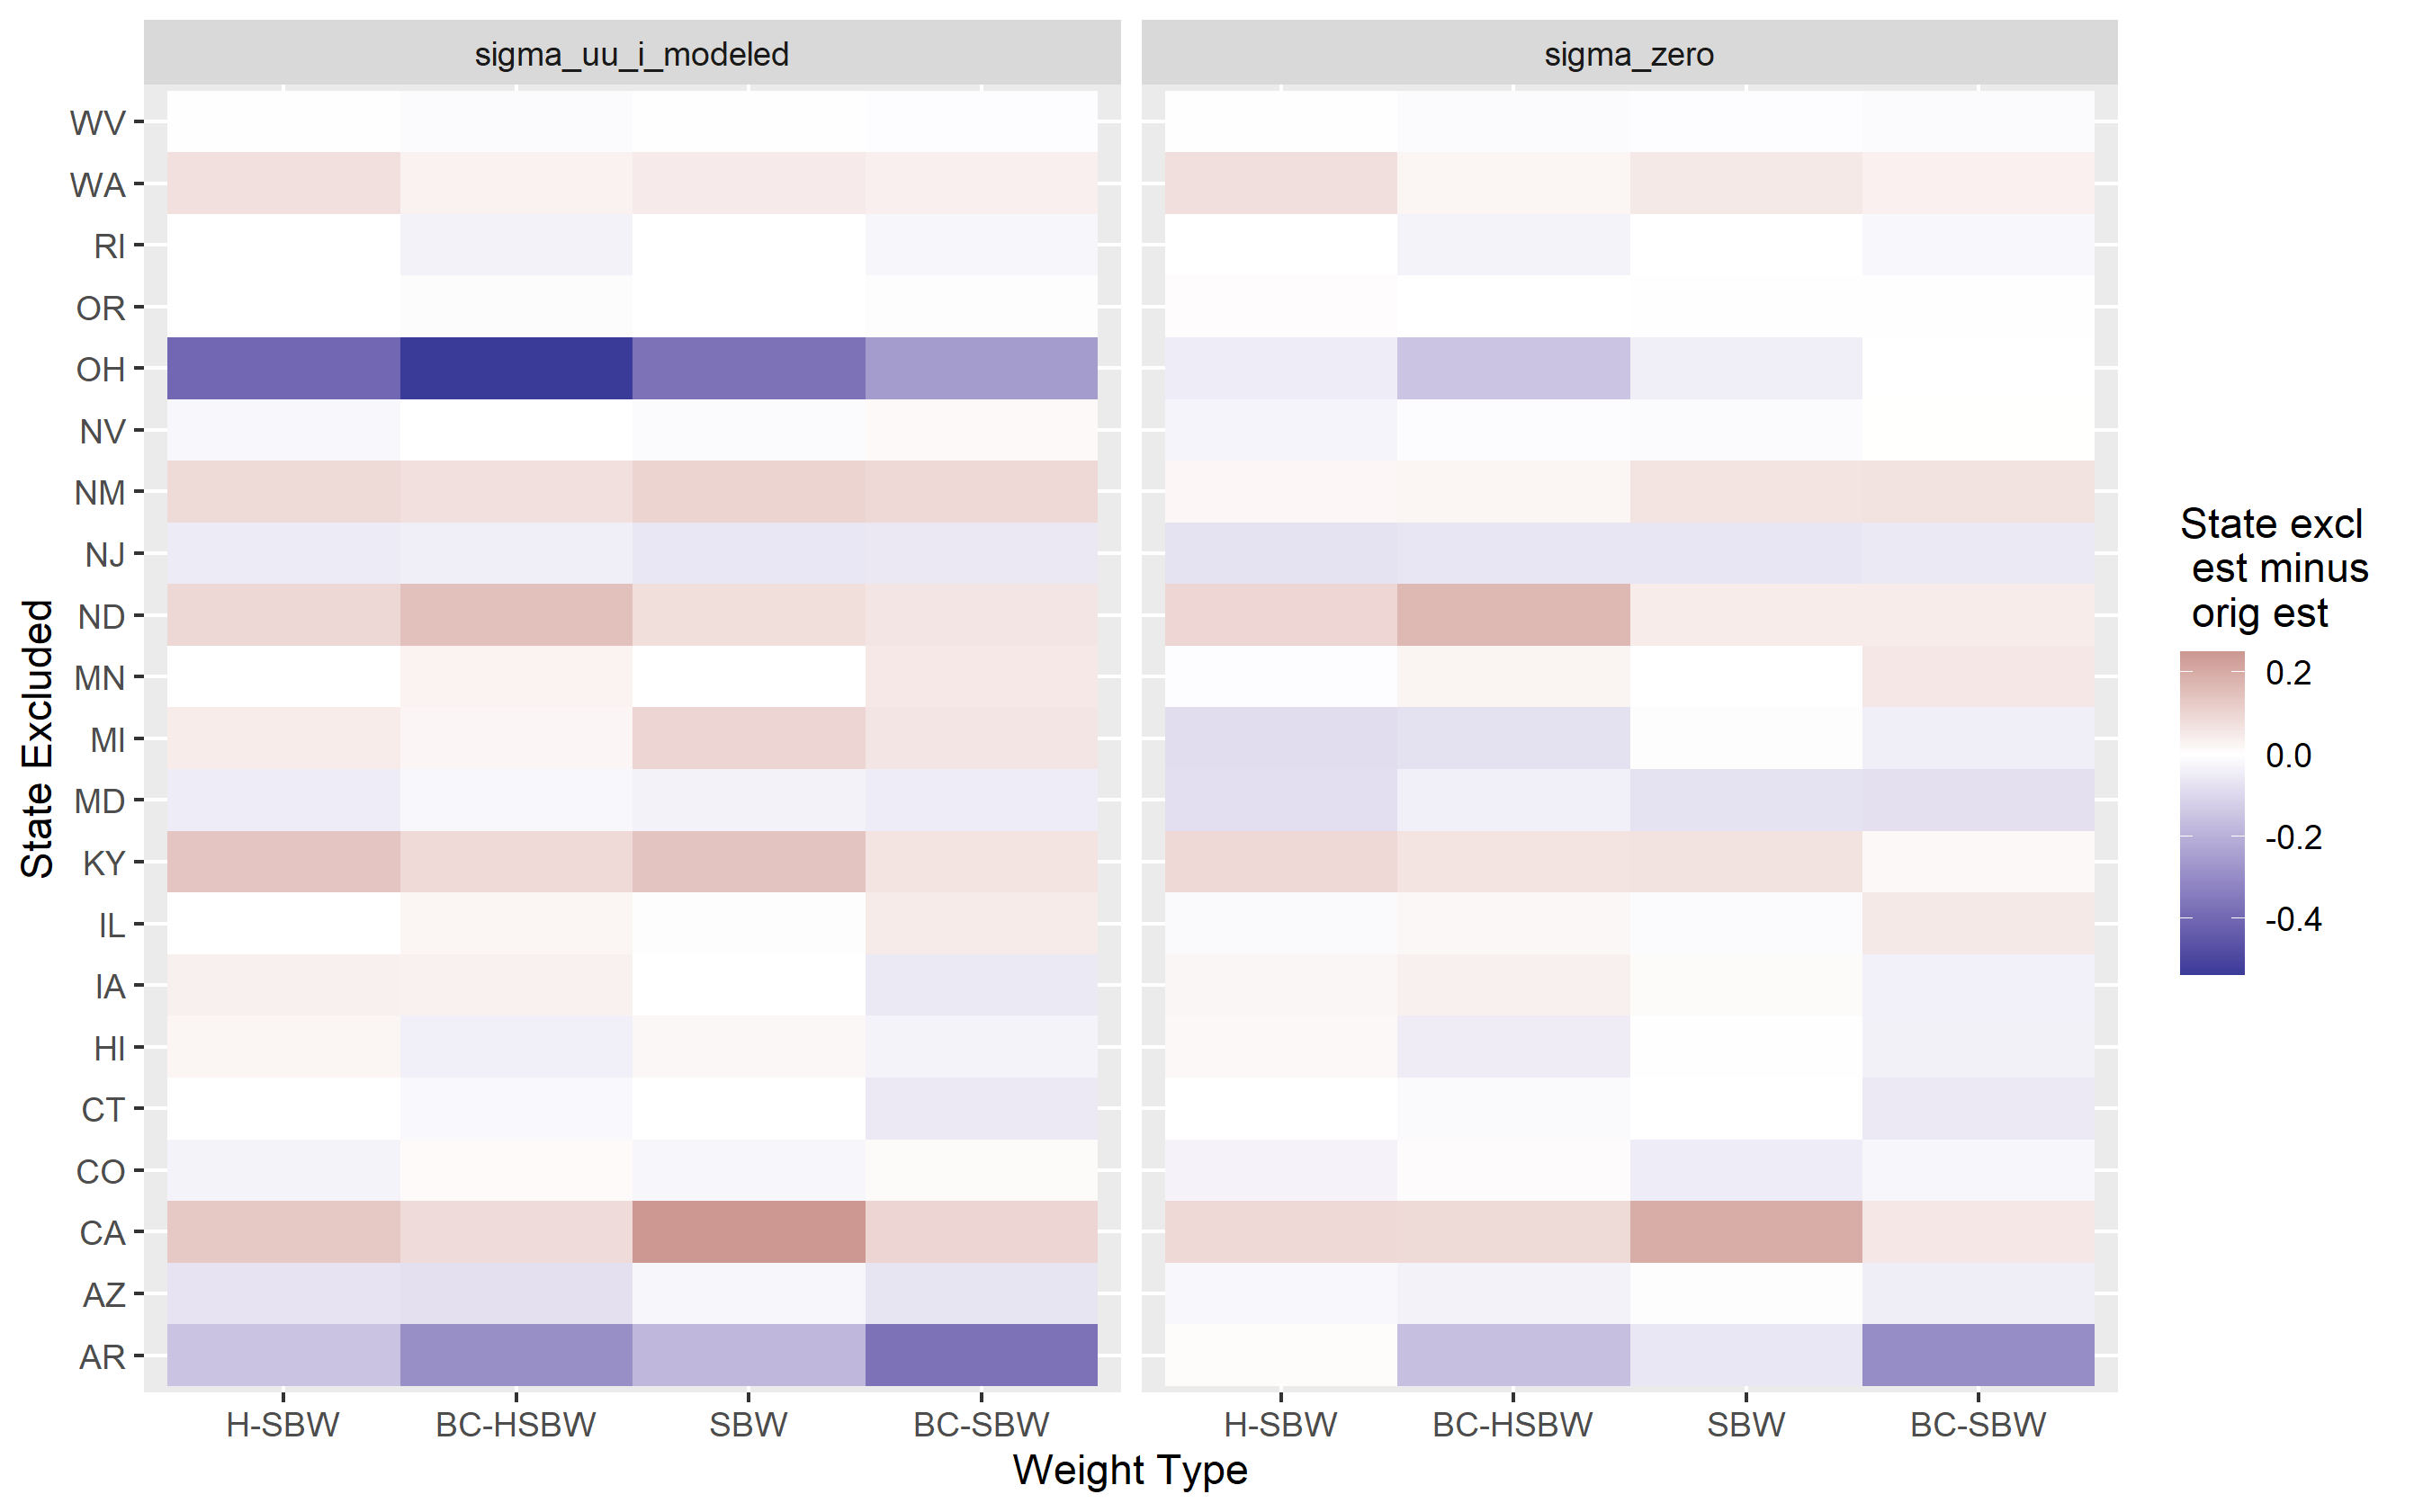
\includegraphics[scale=0.6]{01_Plots/loostate-sensitivityc1-state-uu-i.png}
\end{center}
\end{figure}

\subsection{Covariate importance}

We also investigate our hypothesis that factors associated with Governance are associated with treatment response. As discussed above, we first remove the balance constraints on the Republican governance indicators and estimate $\hat{\psi}^1_v$, and then subtract our original ETC point estimate from this quantity to generate $\hat{\Delta}_v^1$. Because this quantity does not reflect a clear population target, instead of confidence intervals, we present the minimum and maximum leave-one-state-out values in parentheses next to the original estimate.

For the H-SBW estimator we calculate $\hat{\Delta}^1$ equal to -0.69 (min = -0.83, max = -0.42) and equal to -0.79 (min = -0.90, max = -0.66) on our unadjusted dataset. In other words, our primary estimated treatment effect moved 0.78 percentage points further away from zero when we excluded the Republican governance indicators. This reflects a 33 percent decrease in our point estimate, a not-unsubstantial difference. Moreover, all of these estimates were less than zero, regardless of whether we conditioned on the covariate adjustment or not, regardless of whether we remove the early expansion states or not, and when removing each state. Across all specifications that we ran the minimum change we calculated was -1.34 and the maximum was -0.36. Additional distributional results across all leave-one-state-out estimates are available in Appendix E, Table~\ref{tab:rdiffc1}. Figure~\ref{fig:repub} displays our estimates of $\hat{\Delta}_v^1$ on our primary dataset and removing early expansion states (conditional on the covariate adjustment). 

We also consider four other covariate sets. We find that our estimates are most sensitive to controlling for pre-treatment outcomes and unemployment rates. This is not unexpected: all else equal, the expansion region had much lower pre-treatment uninsurance rates. If we do not control for these covariates, the comparable region will likely have lower pre-treament uninsurance rates, causing the estimated counterfactual to be closer to zero. The effect estimates were less sensitive to the removal of other covariate groups, and all point estimates are available in Appendix E, Table~\ref{tab:ptests}.

\begin{figure}[H]
\begin{center}
    \caption{Removing Republican Governance Indicators}
    \label{fig:repub}
    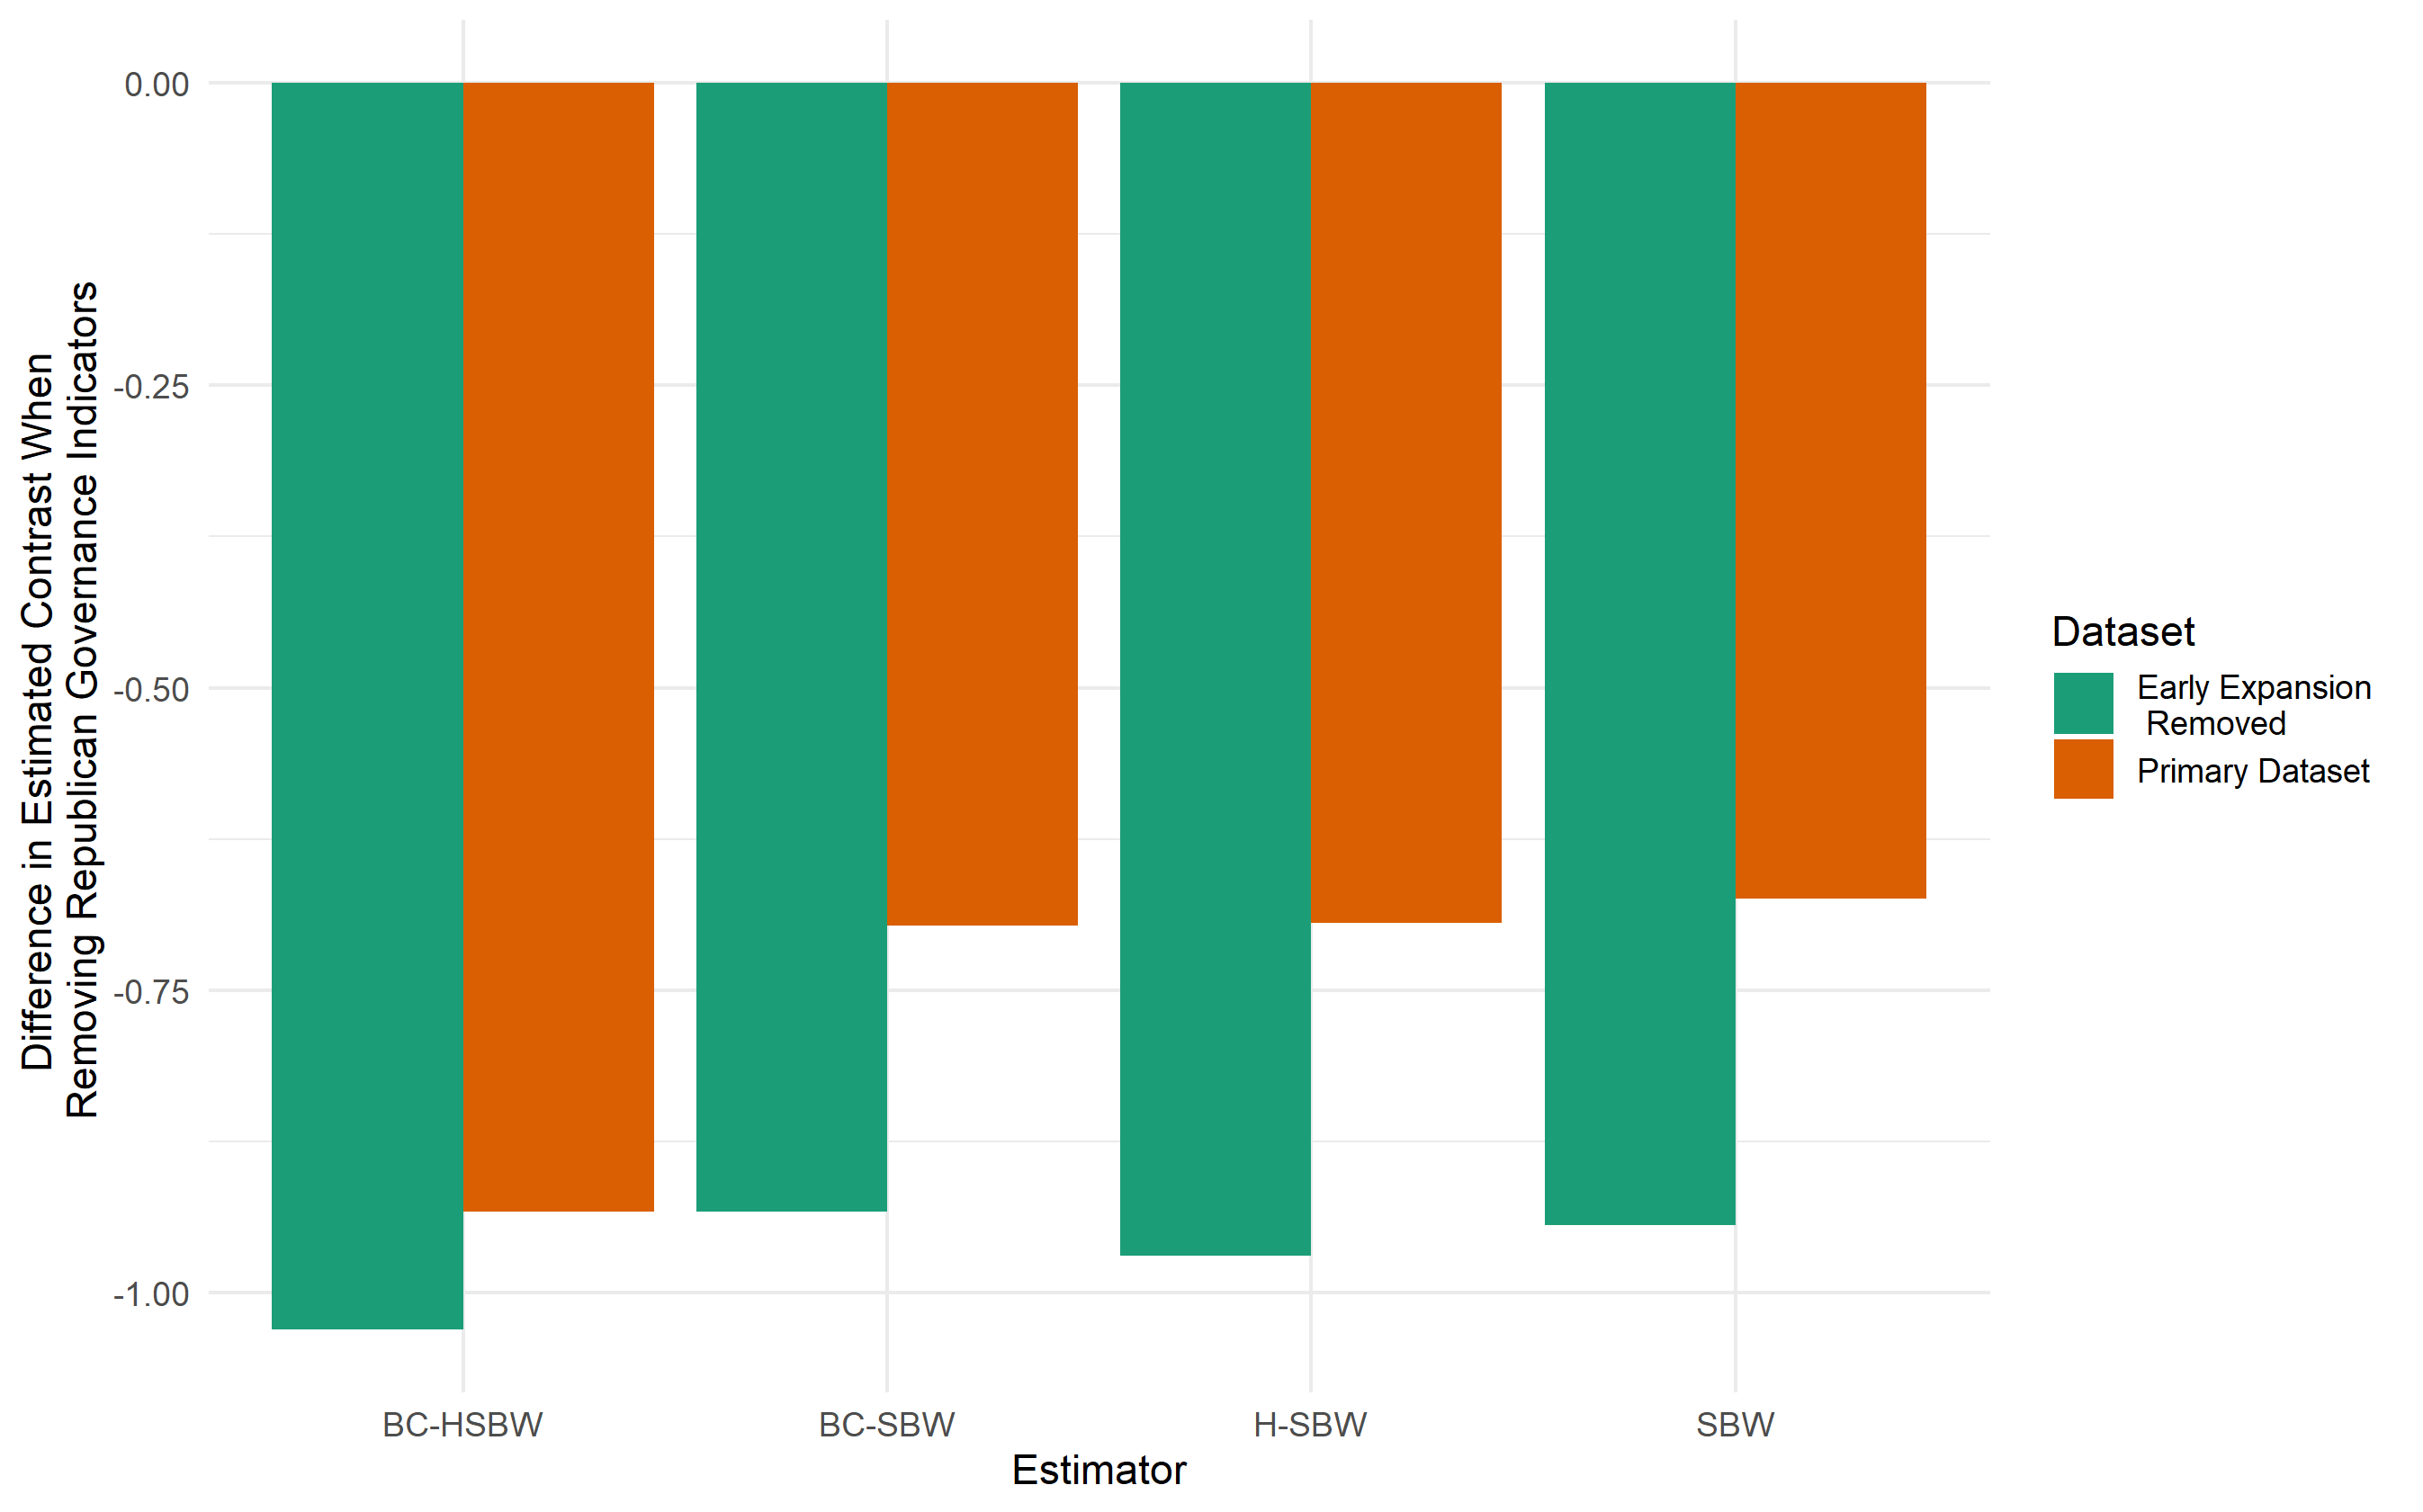
\includegraphics[scale=0.6]{01_Plots/repub-diff-all-estimators.png}
\end{center}
\end{figure}

These results highlight the importance of Republican governance in our counterfactual outcome model of $Y^1$. If the models specified by \cite{kaestner2017effects} and \cite{courtemanche2017early} are correct (that is, they correctly omit Republican governance from their balancing weights for estimating $\bar{Y}^0_{1, T}$), this would suggest treatment effect heterogeneity with respect to Republican governance. Moreover, because the expansion-state region is much more Democratic than the non-expansion region, this heterogeneity could potentially drive differences between the ETC and the ETT.

Since this is a policy question of some interest, we directly investigate this by estimating the outcome model on the full data with treatment assignment interacted with each covariate \footnote{For this analysis we calculate separate covariate adjustments on the untreated data. The summary statistics for this adjustment are available in Appendix D.}. We then examine how the estimated treatment effect would change if we decreased the interaction between treatment assignment and each Republican governance indicator -- Republican governor, Republican lower legislature control, and Republican total control -- by 50 percentage points (the original variables are either 0 or 100 and are measured at the state level). This linear combination of coefficients estimates how the treatment effect would change for any given collection of states against a set that is identical except for being 50 percentage points lower, on average, across the Republican governance indicators. We find that the linear combination is positive (0.21 percentage points) and statistically significant at the 5 percent level on the unadjusted dataset. In contrast to our previous results, this would indicate that the estimated treatment effect may be larger among Republican governed areas. However, this finding is not robust to any other specification that we run. Ultimately we interpret these results as providing no evidence of treatment effect heterogeneity with respect to Republican governance. The full results are available in Appendix E, Table~\ref{tab:hte}.




\end{document}
